%----------------------------------------------------------------------------------------
%	PACKAGES AND DOCUMENT CONFIGURATIONS
%----------------------------------------------------------------------------------------
\documentclass[12pt,a4paper]{report}

\usepackage{geometry} % To set page size and margins accurately
\usepackage{siunitx} % Provides the \SI{}{} and \si{} command for typesetting SI units
\usepackage{graphicx} % Required for the inclusion of images
\usepackage{amsmath} % Required for some math elements 
\usepackage{paralist} % For compactitem lists
\usepackage{color} % Color management options
\usepackage{listings} % To typeset source code
\usepackage{pdflscape} % Landscape pages
\usepackage{acro} %To create acronyms lists
\usepackage{pgfplots}
\usepackage{tabu}
\usepackage{longtable}
\usepackage[strings]{underscore}
\usepackage{pdfpages}
\usepackage[hidelinks]{hyperref}
\usepackage[backend=biber, style=ieee]{biblatex}
\usepackage{tikz}
\usepackage{pifont}
\usepackage{caption}
\usepackage{subcaption}
\usepackage{textcomp}
\usepackage{multicol}
\usepackage{adjustbox}
\usepackage{array}

\tikzset{every picture/.style={line width=0.75pt}} %set default line width to 0.75pt        

\addbibresource{references.bib}

\setcounter{secnumdepth}{3}

\newcolumntype{R}[2]{%
	>{\adjustbox{angle=#1,lap=\width-(#2)}\bgroup}%
	l%
	<{\egroup}%
}
\newcommand*\rot[2]{\multicolumn{1}{R{#1}{#2}}}

\geometry{
	a4paper,
	total={160mm,247mm},
	left=30mm,
	top=25mm
}
\setlength\parindent{0.5cm} % Set indentation for paragraphs
% To make floats, on float only pages, placed at top.
\makeatletter
	\setlength{\@fptop}{0pt}
	\setlength{\@fpbot}{0pt plus 1fil}
\makeatother

%----------------------------------------------------------------------------------------
%	ACRONYMS AND SYMBOLS
%----------------------------------------------------------------------------------------
% class `abbrev': abbreviations:
\DeclareAcronym{uc}{
	short = $\mu$C ,
	long  = Micro-Controller ,
	short-plural = s ,
	long-plural = s ,
	class = abbrev
}
\DeclareAcronym{led}{
	short = LED ,
	long  = Light-Emitting Diode ,
	short-plural = s ,
	long-plural = s ,
	class = abbrev
}
\DeclareAcronym{sipo}{
	short = SIPO ,
	long  = Serial In Parallel Out ,
	class = abbrev
}
\DeclareAcronym{piso}{
	short = PISO ,
	long  = Parallel In Serial Out ,
	class = abbrev
}
\DeclareAcronym{pcb}{
	short = PCB ,
	long  = Printed Circuit Board ,
	short-plural = 's ,
	long-plural = s ,
	class = abbrev
}
\DeclareAcronym{midi}{
	short = MIDI ,
	long  = Musical Instrument Digital Interface,
	class = abbrev
}
\DeclareAcronym{daw}{
	short = DAW ,
	long  = Digital Audio Workstation,
	short-plural = 's ,
	long-plural = s ,
	class = abbrev
}
\DeclareAcronym{usb}{
	short = USB ,
	long  = Universal Serial Bus,
	class = abbrev
}
\DeclareAcronym{spi}{
	short = SPI ,
	long  = Serial Peripheral Interface,
	class = abbrev
}
\DeclareAcronym{i2c}{
	short = I$^2$C ,
	long  = Inter-Integrated Circuit,
	class = abbrev
}
\DeclareAcronym{i2s}{
	short = I$^2$S ,
	long  = Inter-IC Sound,
	class = abbrev
}
\DeclareAcronym{ic}{
	short = IC ,
	long  = Integrated Circuit,
	short-plural = s ,
	long-plural = s ,
	class = abbrev
}
\DeclareAcronym{otg}{
	short = OTG ,
	long  = On The Go,
	class = abbrev
}
\DeclareAcronym{dac}{
	short = DAC ,
	long  = Digital to Analog Converter,
	short-plural = s ,
	long-plural = s ,
	class = abbrev
}
\DeclareAcronym{adc}{
	short = ADC ,
	long  = Analog to Digital Converter,
	short-plural = s ,
	long-plural = s ,
	class = abbrev
}
\DeclareAcronym{lcd}{
	short = LCD ,
	long  = Liquid Crystal Display,
	short-plural = s ,
	long-plural = s ,
	class = abbrev
}
\DeclareAcronym{mux}{
	short = mux ,
	long  = multiplexer,
	short-plural = s ,
	long-plural = s ,
	class = abbrev
}
\DeclareAcronym{fsm}{
	short = FSM ,
	long  = Finite State Machine,
	short-plural = s ,
	long-plural = s ,
	class = abbrev
}
\DeclareAcronym{cpu}{
	short = CPU ,
	long  = Central Processing Unit,
	short-plural = s ,
	long-plural = s ,
	class = abbrev
}
\DeclareAcronym{riff}{
	short = RIFF ,
	long  = Resource Interchange File Format,
	short-plural = s ,
	long-plural = s ,
	class = abbrev
}
\DeclareAcronym{gpio}{
	short = GPIO ,
	long  = General Purpose Input-Output,
	class = abbrev
}
\DeclareAcronym{bpm}{
	short = BPM ,
	long  = Beats per Minute,
	class = abbrev
}
\DeclareAcronym{uart}{
	short = UART ,
	long  = Universal Asynchronous Receiver/Transmitter,
	class = abbrev
}
\DeclareAcronym{ac}{
	short = AC ,
	long  = Alternating Current,
	class = abbrev
}
\DeclareAcronym{dc}{
	short = DC ,
	long  = Direct Current,
	class = abbrev
}
\DeclareAcronym{dma}{
	short = DMA ,
	long  = Direct Memory Access,
	class = abbrev
}
\DeclareAcronym{pcm}{
	short = PCM ,
	long  = Pulse-Code Modulation,
	class = abbrev
}
\DeclareAcronym{ram}{
	short = RAM ,
	long  = Random Access Memory,
	class = abbrev
}
\DeclareAcronym{fat}{
	short = FAT ,
	long  = File Allocation Table,
	class = abbrev
}
\DeclareAcronym{fatfs}{
	short = FATFS ,
	long  = \ac{fat} File System,
	class = abbrev
}
\DeclareAcronym{baud}{
	short = Bd ,
	long  = baud,
	class = abbrev
}
\DeclareAcronym{usart}{
	short = USART ,
	long  = Universal Synchronous/Asynchronous Receiver/Transmitter,
	class = abbrev
}
\DeclareAcronym{ascii}{
	short = ASCII ,
	long  = American Standard Code for Information Interchange,
	class = abbrev
}
%----------------------------------------------------------------------------------------
%	DOCUMENT INFORMATION AND TITLE PAGE
%----------------------------------------------------------------------------------------
\renewcommand{\thepage}{Cover}
\title{Simple Beat Matrix \\ Sequential Drum Machine } % Title

\author{Pieter \textsc{Goos}} % Author name

\date{\today} % Date for the report

\makeatletter
\let\thetitle\@title
\let\theauthor\@author
\let\thedate\@date
\makeatother

\begin{document}

\begin{titlepage}
    \centering
    \vspace*{0.5 cm}
    
\includegraphics[scale = 2]{EELogo.png}\\[1.0 cm]   % University Logo
    \vspace{3cm}
    \rule{\linewidth}{0.2 mm} \\[0.4 cm]
    { \huge \bfseries \thetitle }\\[0.4 cm]
    \rule{\linewidth}{0.2 mm} \\[1.5 cm]
    \vspace{2cm}
	\begin{minipage}{6.5cm}
		\begin{flushleft} \large
			\emph{Student Name:}\\
			\emph{Student Number:}\\
			\emph{Study Leader:}\\
			\emph{Date:}
		\end{flushleft}
	\end{minipage}~
	\begin{minipage}{6.5cm}
		\begin{flushright} \large
		\theauthor\\
		19231466-2015\\
		Dr. Lourens \textsc{Visagie}\\
		June 2019
		\end{flushright}
	\end{minipage}\\[2 cm]
    \vfill
    
\includegraphics[width=7cm]{SUNLogo.jpg}\\[1.0 cm]
    Report submitted in partial fulfilment of the requirements of the module Project (E) 448 for the degree Baccalaureus in Engineering in the Department of Electrical and Electronic Engineering at the University of Stellenbosch.
    
\end{titlepage}

%----------------------------------------------------------------------------------------
%	Acknowledgements
%----------------------------------------------------------------------------------------
\pagenumbering{Roman}
\addcontentsline{toc}{chapter}{Preamble}
\section*{Acknowledgements}
\addcontentsline{toc}{section}{Acknowledgements}
Firstly a thank you goes to Dr. L. Visagie for allowing me to pursue this topic in the first semester as well as all the guidance provided. \\\\
Further thank you goes to Wynand van Eeden for the knowledge of PCBs and patience with all the 3D prints.\\\\
I would like to thank my girlfriend, Daena Voges, for standing by my side over the past years and dealing with all of my ramblings and frustrations. You have given me nothing but love and support over not only this project, but since the beginning of my studies.\\\\
My friends, thank you for the laughter and help you've given me. Particularly Richard Batt, having someone share this journey with nothing but jokes has been a lifesaver; and Alex Faustmann for the support and keeping me earthed for the future.\\\\
To my mother, Catty Goos, thank you for all the support you have given me over all these years and allowing me to study what I wanted with all the support I needed.\\\\
Finally, my dad, Danny Goos $\dagger$, thank you for all your sit down talks and motivation boosters over the years. I miss you and I know you'd be proud of how far I've come. \textit{Uw maateke is er geraakt, op naar het volgende advontuur, Love you!}
\newpage

%----------------------------------------------------------------------------------------
%	DECLARATION
%----------------------------------------------------------------------------------------
\addcontentsline{toc}{section}{Plagiarism Declaration}
\section*{Plagiarism Declaration / Plagiaatverklaring}
\begin{enumerate}
\item Plagiarism is the use of ideas, material and other intellectual property of another's work and to present is as my own. \newline \textit{Plagiaat is die oorneem en gebruik van die idees, materiaal en ander intellektuele eiendom van ander persone asof dit jou eie werk is.} 
\item I agree that plagiarism is a punishable offense because it constitutes theft. \newline \textit{Ek erken dat die pleeg van plagiaat 'n strafbare oortreding is aangesien dit ‘n vorm van diefstal is. }
\item I also understand that direct translations are plagiarism. \newline \textit{Ek verstaan ook dat direkte vertalings plagiaat is. }
\item Accordingly all quotations and contributions from any source whatsoever (including the internet) have been cited fully. I understand that the reproduction of text without quotation marks (even when the source is cited) is plagiarism. \newline \textit{Dienooreenkomstig is alle aanhalings en bydraes vanuit enige bron (ingesluit die internet) volledig verwys (erken). Ek erken dat die woordelikse aanhaal van teks sonder aanhalingstekens (selfs al word die bron volledig erken) plagiaat is. }
\item I declare that the work contained in this assignment, except where otherwise stated, is my original work and that I have not previously (in its entirety or in part) submitted it for grading in this module/assignment or another module/assignment. \newline \textit{Ek verklaar dat die werk in hierdie skryfstuk vervat, behalwe waar anders aangedui, my eie oorspronklike werk is en dat ek dit nie vantevore in die geheel of gedeeltelik ingehandig het vir bepunting in hierdie module/werkstuk of ‘n ander module/werkstuk nie.} 
\end{enumerate}
\vspace{1cm}
\begin{table}[ht]
	\begin{center}
		\begin{tabular*}{15.5cm}{@{\extracolsep{\fill}}lll}
			\makebox[8cm]{\hrulefill} & & \makebox[6cm]{\hrulefill}\\
			%\hrulefill & & \hrulefill \\
			Signature & & Student number \\
			\textit{Handtekening} & & \textit{Studentenommer} \\[1cm]
		    \makebox[8cm]{\hrulefill} & & \makebox[6cm]{\hrulefill}\\ 
			%\hrulefill & & \hrulefill\\
			Initials and surname & & Date \\
			\textit{Voorletters en van} & & \textit{Datum}\\
		\end{tabular*}
	\end{center}
\end{table}

\vfill

\begin{center}
	Copyright \textcopyright \space Stellenbosch University 2019\\
	All Rights Reserved
\end{center}

\newpage

%----------------------------------------------------------------------------------------
%	Summary
%----------------------------------------------------------------------------------------
\addcontentsline{toc}{section}{Summary / Opsomming}
\section*{Summary}
A drum machine allows for a musician to sequence multiple percussion sounds without the need for a drum kit or a drummer. This report not only focuses on the history, and thus the different variants of a drum machine, but also the design decisions made for not only hardware but also software. Every component is first designed in hardware and then driven by a controller through software. Each subsection of the system is discussed in detail, with various options on how to achieve similar results mentioned and explored. Measurements coming from the various parts of the device are shown and discussed. All of this cumulating to a finished, working, design allowing a user to schedule and play back their own sounds on a compact drum machine. 
\section*{Opsomming}
'n Drommasjien maak dit vir 'n musikant moontlik om verskeie perkussie geluide te orden sonder dat daar 'n dromstel of drommer nodig is. Hierdie verslag fokus nie net op die geskiedenis, en dus ook die verskillende veriante van 'n drommasjien, nie, maar ook op die ontwerpbesluite wat nie net vir hardeware gemaak is nie, maar ook vir sagteware. Elke komponent is eers ontwerp as hardeware en deur middel van 'n beheerder bestuur via sagteware. Elke onderafdeling van die stelsel word in detail bespreek, met verskeie opsies oor hoe om soortgelyke resultate te verkry en gebruik. Mate, wat van die verskillende dele van die toestel kom, word getoon en bespreek. Al hierdie versamel mooi tot 'n voltooide en werkende ontwerp wat 'n gebruiker toelaat om hul eie klank monsters op 'n kompakte drommasjien te skeduleer en hoor.
\newpage

%----------------------------------------------------------------------------------------
%	TOC, Lists (Figures, Tables etc)
%----------------------------------------------------------------------------------------
\tableofcontents
\listoffigures
\listoftables
\lstlistoflistings
\newpage
%Acronym lists
\chapter*{List of Abbreviations}
\begin{multicols}{2}
	\printacronyms[name={List of Abbreviations}, heading=none]
\end{multicols}

\newpage

%----------------------------------------------------------------------------------------
%	SECTION 1
%----------------------------------------------------------------------------------------
\pagenumbering{arabic}
\chapter{Introduction}
\section{Project Background}
Drum machines aid musicians by allowing them to generate drum, or other percussion, sounds on a schedule without a drum kit. Modern drum machines allow for the musician to program their own rhythms into the device. Since the beginnings of the drum machine in the 1930s \cite{rhythmart} the functionality has evolved in many ways. Several different programming and scheduling techniques are used by different manufacturers. \\\\
The first style of programmable drum machines placed different sounds in the rows and consecutive time steps in the columns \cite{rhythmart, beatgoeson}. This drum machine will essentially act as a sequencer as it steps over the time steps repeatedly. This is the style of drum machine that will be used for this project as it proves one of the simplest to understand for new users. Some features will be added on top of the designs from the 1970s \cite{rhythmart, beatgoeson} by using more modern luxuries such as a display and the ability to use one's own audio samples.
\section{Project Aims} \label{sec:specs}
The aims of this project are as follows:
\begin{itemize}
	\setlength\itemsep{0em}
	\item Design and Manufacture a controllable matrix of indicators to schedule audio sample playback
	\item Design and Manufacture a method for the user to hear the sequenced samples
	\item Design and Manufacture a method to change the tempo and volume of the sequenced samples
	\item Have the ability to indicate the current state of the device's volume, tempo, and position in the sequence
	\item Design and Manufacture a \ac{pcb} for the system
	\item Design and Manufacture an enclosure for the completed system
	\item Select a \ac{uc} for controlling all of the device's features
	\item Design and implement a method for a \ac{usb} Storage Device to store the audio samples
\end{itemize}
%----------------------------------------------------------------------------------------
%	SECTION 2
%----------------------------------------------------------------------------------------
\chapter{Background on Drum Machines}
To design a drum machine one must first determine what that is and could be. Unfortunately it is not as straight-forward as one would believe as there are several forms of drum machines. The complexity and mere perception of what it is have changed since its beginnings in the 1930s, thus a point in time will need to be selected to be the basis of this project.
\section{The Beginning of Drum Machines}
Before drum machines could be programmed to the musician's liking it would make simple or pre-recorded sounds on a schedule. This meant that the \textit{drum machines} of the time, the 1930s into the 1950s, acted mostly as timing to be used in conjunction with other instruments \cite{rhythmart}. \\
The earliest device one could conceive as a drum machine was the \textit{Rhythmicon} by L\'eon Theremin and commissioned by Henry Cowell \cite{rhythmart, beatgoeson}. The \textit{Rhythmicon} was completed in 1931 and could only produce sixteen different rhythms \cite{schedel}. These rhythms would all be more rapid than the previous, all based on a periodic base rhythm. This device would, however, only act as a concept for the next two decades. \\
In the late 1950s, large devices such as the \textit{Chamberlin Rhythmate} or the \textit{Wurlitzer Sideman} came on the market. These two offered a more pleasant sound to listen to by playing back audio tapes (at various speeds), and a system similar to a music box respectively \cite{rhythmart, beatgoeson}. The latter, the \textit{Sideman}, had rhythmic styles including the Samba, Waltz and more\cite{WangOliver2014Htdm}. \\
Progressing to the 1960s, drum machines started to be manufactured with, at the time, new solid-state transistors. These transistors allowed the units to shrink in size drastically. In Japan, a new trend was encouraged by companies such as Ace Tone, and Keio-Giken to create organ accessories. Outside of Japan, the idea would be taken in a different perspective by creating pre-set rhythm boxes, such as the \textit{Elka Drummer One}. For these devices to progress, a new level of control would be required \cite{rhythmart}.
\section{Programmable Drum Machines}
First one will have to understand what is meant by \textit{programmable}: this refers to the ability for musicians to create their own patterns of internal sounds \cite{rhythmart}.\\
\begin{figure}[h!]
	\begin{center}
		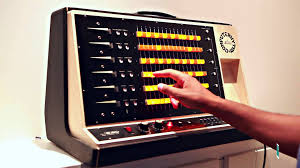
\includegraphics[width = 0.5\textwidth, angle=0, origin=c]{computerhythm.jpg}
		\caption{An Eko Compute Rhythm in Use \cite{comprhythImg}}
		\label{fig:comprhyt}
	\end{center}
\end{figure}
The first programmable drum machines came about in the 1970s with the \textit{Eko Compute Rhythm} in 1972, as seen in Figure \ref{fig:comprhyt}. This product featured a beat matrix, something that can still be found today \cite{beatgoeson}. Beat Matrices will be discussed in Section \ref{sec:beatmatrix}. Roland introduced the first drum machine to feature a microprocessor in 1978 with the \textit{CR-78 CompuRhythm}. This allowed the user to store entire sequences \cite{cr78}. Several years later they brought out the \textit{TR-808} with a set of programmable synthesized analogue sounds \cite{tr808, beatgoeson}. At this point, the demand for real drum sounds was high and thus came the Sample-Based Drum Machines.\\
In 1980, the \textit{Linn Electronics LM-1} was released to be the first drum machine to use recorded samples as opposed to synthesized sounds \cite{beatgoeson}. Synth manufacturers began to enter the rhythmic device market with a product that made use of swappable memory cards, had \ac{midi} integration, among other features \cite{rhythmart}.\\
The most important feature to be added in the forthcoming years was being able to sample sounds on the device itself. This was pioneered by the \textit{Akai MPC} series of drum machines. These featured sixteen responsive pad controllers and had all the features of a drum machine \cite{beatgoeson, rhythmart}. This wave of new machines throughout the 1980s paved the way for 'stations' such as the more recent \textit{Native Instruments Maschine} series \cite{rhythmart}, an example of which can be seen in Figure \ref{fig:maschine}.\\
\begin{figure}[h!]
	\begin{center}
		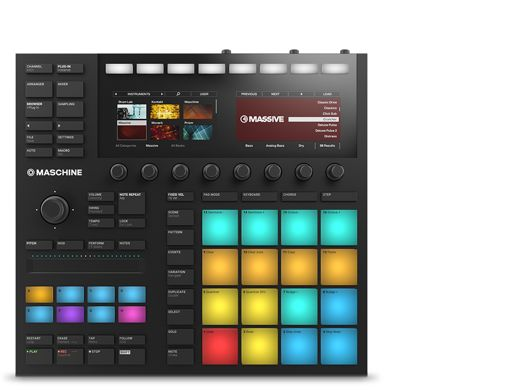
\includegraphics[width = 0.4\textwidth, angle=0, origin=c, trim={0 0 140px 35px}, clip]{maschine.jpg}
		\caption{Native Instruments Maschine Mk3 \cite{maschine}}
		\label{fig:maschine}
	\end{center}
\end{figure}
\section{Beat Matrices}\label{sec:beatmatrix}
A beat matrix is a term used to describe how different sounds are scheduled and indicated on certain types of drum machines or sound sequencers. Each row is a different sound, or beat, that can be sequenced on each column. In other words, each row represents a sound and each column a time step. An indicator will progress over the matrix's columns to show the current beat that is being played. In Figure \ref{fig:beatmatrixex} a simple inverted column indicator is used, meaning that if a sound in this column is selected the indicator will not show here if a is sound is not selected then the indicator will show. Alternatively, a separate indicator can be used to indicate the currently selected column. As the indicator column shifts right, to the next column, the sounds from each row that are selected in the current column will be played simultaneously. The pattern of sounds that are scheduled repeats once the indicator reaches the last column. The indicator column will then wrap around when it comes time to progress to the next step and indicate the first column again. The user has full control over which sounds will be scheduled at any given point on the grid by simply selecting a sound (row) at a given point in the sequence (column). 
\begin{figure}[h!]
	\centering
	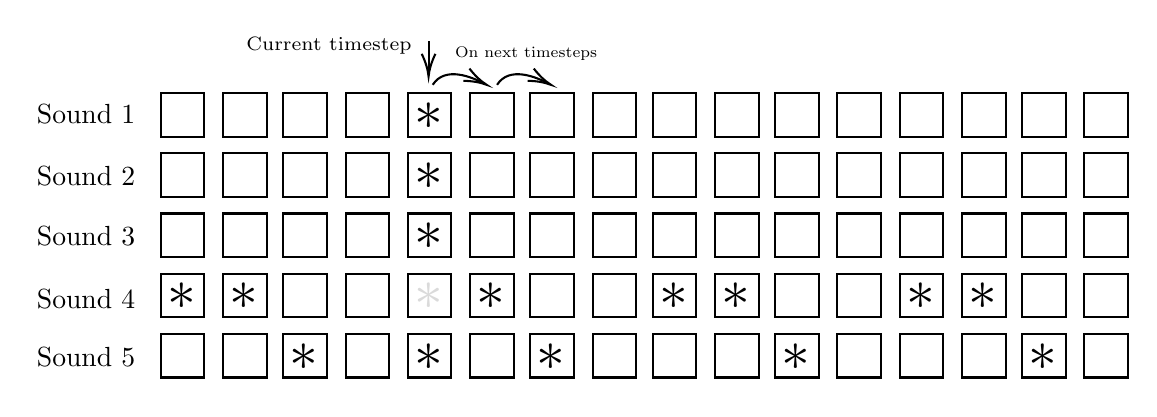
\begin{tikzpicture}[x=0.75pt,y=0.75pt,yscale=-1,xscale=1]
	%uncomment if require: \path (0,300); %set diagram left start at 0, and has height of 300
	
	%Shape: Square [id:dp055075823113389655] 
	\draw   (71,57) -- (92,57) -- (92,78) -- (71,78) -- cycle ;
	%Shape: Square [id:dp1704678574916212] 
	\draw   (71,86) -- (92,86) -- (92,107) -- (71,107) -- cycle ;
	%Shape: Square [id:dp07556141052574583] 
	\draw   (71,115) -- (92,115) -- (92,136) -- (71,136) -- cycle ;
	%Shape: Square [id:dp6450747332533515] 
	\draw   (71,144) -- (92,144) -- (92,165) -- (71,165) -- cycle ;
	%Shape: Square [id:dp5261271526192695] 
	\draw   (71,173) -- (92,173) -- (92,194) -- (71,194) -- cycle ;
	%Shape: Square [id:dp9693004806617898] 
	\draw   (101,57) -- (122,57) -- (122,78) -- (101,78) -- cycle ;
	%Shape: Square [id:dp015245941871381286] 
	\draw   (101,86) -- (122,86) -- (122,107) -- (101,107) -- cycle ;
	%Shape: Square [id:dp09796296192393927] 
	\draw   (101,115) -- (122,115) -- (122,136) -- (101,136) -- cycle ;
	%Shape: Square [id:dp19512834167257576] 
	\draw   (101,144) -- (122,144) -- (122,165) -- (101,165) -- cycle ;
	%Shape: Square [id:dp12372448635059285] 
	\draw   (101,173) -- (122,173) -- (122,194) -- (101,194) -- cycle ;
	%Shape: Square [id:dp018256335768894294] 
	\draw   (130,57) -- (151,57) -- (151,78) -- (130,78) -- cycle ;
	%Shape: Square [id:dp9302456652282582] 
	\draw   (130,86) -- (151,86) -- (151,107) -- (130,107) -- cycle ;
	%Shape: Square [id:dp0743061274063912] 
	\draw   (130,115) -- (151,115) -- (151,136) -- (130,136) -- cycle ;
	%Shape: Square [id:dp7787868056907525] 
	\draw   (130,144) -- (151,144) -- (151,165) -- (130,165) -- cycle ;
	%Shape: Square [id:dp7408580081312215] 
	\draw   (130,173) -- (151,173) -- (151,194) -- (130,194) -- cycle ;
	%Shape: Square [id:dp06415229039380055] 
	\draw   (160,57) -- (181,57) -- (181,78) -- (160,78) -- cycle ;
	%Shape: Square [id:dp4482970084197244] 
	\draw   (160,86) -- (181,86) -- (181,107) -- (160,107) -- cycle ;
	%Shape: Square [id:dp22938505936887] 
	\draw   (160,115) -- (181,115) -- (181,136) -- (160,136) -- cycle ;
	%Shape: Square [id:dp24930733054102783] 
	\draw   (160,144) -- (181,144) -- (181,165) -- (160,165) -- cycle ;
	%Shape: Square [id:dp8100175607090523] 
	\draw   (160,173) -- (181,173) -- (181,194) -- (160,194) -- cycle ;
	%Shape: Square [id:dp11884312408151132] 
	\draw   (190,57) -- (211,57) -- (211,78) -- (190,78) -- cycle ;
	%Shape: Square [id:dp07651067247882515] 
	\draw   (190,86) -- (211,86) -- (211,107) -- (190,107) -- cycle ;
	%Shape: Square [id:dp718935335969201] 
	\draw   (190,115) -- (211,115) -- (211,136) -- (190,136) -- cycle ;
	%Shape: Square [id:dp9548839777289837] 
	\draw   (190,144) -- (211,144) -- (211,165) -- (190,165) -- cycle ;
	%Shape: Square [id:dp6870621310591223] 
	\draw   (190,173) -- (211,173) -- (211,194) -- (190,194) -- cycle ;
	%Shape: Square [id:dp6993734727621279] 
	\draw   (220,57) -- (241,57) -- (241,78) -- (220,78) -- cycle ;
	%Shape: Square [id:dp39388626452428865] 
	\draw   (220,86) -- (241,86) -- (241,107) -- (220,107) -- cycle ;
	%Shape: Square [id:dp09849069216827844] 
	\draw   (220,115) -- (241,115) -- (241,136) -- (220,136) -- cycle ;
	%Shape: Square [id:dp9892672899362978] 
	\draw   (220,144) -- (241,144) -- (241,165) -- (220,165) -- cycle ;
	%Shape: Square [id:dp6726817229111648] 
	\draw   (220,173) -- (241,173) -- (241,194) -- (220,194) -- cycle ;
	%Shape: Square [id:dp4329811630954301] 
	\draw   (249,57) -- (270,57) -- (270,78) -- (249,78) -- cycle ;
	%Shape: Square [id:dp643406915633401] 
	\draw   (249,86) -- (270,86) -- (270,107) -- (249,107) -- cycle ;
	%Shape: Square [id:dp3054280897220467] 
	\draw   (249,115) -- (270,115) -- (270,136) -- (249,136) -- cycle ;
	%Shape: Square [id:dp37404319144826537] 
	\draw   (249,144) -- (270,144) -- (270,165) -- (249,165) -- cycle ;
	%Shape: Square [id:dp9087449281110727] 
	\draw   (249,173) -- (270,173) -- (270,194) -- (249,194) -- cycle ;
	%Shape: Square [id:dp03289088561922715] 
	\draw   (279,57) -- (300,57) -- (300,78) -- (279,78) -- cycle ;
	%Shape: Square [id:dp8477421076056018] 
	\draw   (279,86) -- (300,86) -- (300,107) -- (279,107) -- cycle ;
	%Shape: Square [id:dp9650777757071278] 
	\draw   (279,115) -- (300,115) -- (300,136) -- (279,136) -- cycle ;
	%Shape: Square [id:dp11005584127939194] 
	\draw   (279,144) -- (300,144) -- (300,165) -- (279,165) -- cycle ;
	%Shape: Square [id:dp05010425824687381] 
	\draw   (279,173) -- (300,173) -- (300,194) -- (279,194) -- cycle ;
	%Shape: Square [id:dp3553939886372164] 
	\draw   (308,57) -- (329,57) -- (329,78) -- (308,78) -- cycle ;
	%Shape: Square [id:dp993475603020693] 
	\draw   (308,86) -- (329,86) -- (329,107) -- (308,107) -- cycle ;
	%Shape: Square [id:dp058277924669569714] 
	\draw   (308,115) -- (329,115) -- (329,136) -- (308,136) -- cycle ;
	%Shape: Square [id:dp3715463502502885] 
	\draw   (308,144) -- (329,144) -- (329,165) -- (308,165) -- cycle ;
	%Shape: Square [id:dp2057129616720641] 
	\draw   (308,173) -- (329,173) -- (329,194) -- (308,194) -- cycle ;
	%Shape: Square [id:dp14547383927293156] 
	\draw   (338,57) -- (359,57) -- (359,78) -- (338,78) -- cycle ;
	%Shape: Square [id:dp9308280273118588] 
	\draw   (338,86) -- (359,86) -- (359,107) -- (338,107) -- cycle ;
	%Shape: Square [id:dp8932216390334204] 
	\draw   (338,115) -- (359,115) -- (359,136) -- (338,136) -- cycle ;
	%Shape: Square [id:dp338657779769743] 
	\draw   (338,144) -- (359,144) -- (359,165) -- (338,165) -- cycle ;
	%Shape: Square [id:dp7829955194217109] 
	\draw   (338,173) -- (359,173) -- (359,194) -- (338,194) -- cycle ;
	%Shape: Square [id:dp656297709216783] 
	\draw   (367,57) -- (388,57) -- (388,78) -- (367,78) -- cycle ;
	%Shape: Square [id:dp38518762724354283] 
	\draw   (367,86) -- (388,86) -- (388,107) -- (367,107) -- cycle ;
	%Shape: Square [id:dp7270283030928499] 
	\draw   (367,115) -- (388,115) -- (388,136) -- (367,136) -- cycle ;
	%Shape: Square [id:dp26858945017560876] 
	\draw   (367,144) -- (388,144) -- (388,165) -- (367,165) -- cycle ;
	%Shape: Square [id:dp20895681326975923] 
	\draw   (367,173) -- (388,173) -- (388,194) -- (367,194) -- cycle ;
	%Shape: Square [id:dp5001505546780691] 
	\draw   (397,57) -- (418,57) -- (418,78) -- (397,78) -- cycle ;
	%Shape: Square [id:dp7085863352155919] 
	\draw   (397,86) -- (418,86) -- (418,107) -- (397,107) -- cycle ;
	%Shape: Square [id:dp5678826142337541] 
	\draw   (397,115) -- (418,115) -- (418,136) -- (397,136) -- cycle ;
	%Shape: Square [id:dp21535552439436345] 
	\draw   (397,144) -- (418,144) -- (418,165) -- (397,165) -- cycle ;
	%Shape: Square [id:dp9820083813501623] 
	\draw   (397,173) -- (418,173) -- (418,194) -- (397,194) -- cycle ;
	%Shape: Square [id:dp20662665023781868] 
	\draw   (427,57) -- (448,57) -- (448,78) -- (427,78) -- cycle ;
	%Shape: Square [id:dp1804616310169056] 
	\draw   (427,86) -- (448,86) -- (448,107) -- (427,107) -- cycle ;
	%Shape: Square [id:dp35963049846659945] 
	\draw   (427,115) -- (448,115) -- (448,136) -- (427,136) -- cycle ;
	%Shape: Square [id:dp9296195059318353] 
	\draw   (427,144) -- (448,144) -- (448,165) -- (427,165) -- cycle ;
	%Shape: Square [id:dp4631619190234555] 
	\draw   (427,173) -- (448,173) -- (448,194) -- (427,194) -- cycle ;
	%Shape: Square [id:dp5685445121019017] 
	\draw   (457,57) -- (478,57) -- (478,78) -- (457,78) -- cycle ;
	%Shape: Square [id:dp07712697453645379] 
	\draw   (457,86) -- (478,86) -- (478,107) -- (457,107) -- cycle ;
	%Shape: Square [id:dp7720907067801506] 
	\draw   (457,115) -- (478,115) -- (478,136) -- (457,136) -- cycle ;
	%Shape: Square [id:dp612829720126973] 
	\draw   (457,144) -- (478,144) -- (478,165) -- (457,165) -- cycle ;
	%Shape: Square [id:dp1744262529005769] 
	\draw   (457,173) -- (478,173) -- (478,194) -- (457,194) -- cycle ;
	%Shape: Square [id:dp10583229890256263] 
	\draw   (486,57) -- (507,57) -- (507,78) -- (486,78) -- cycle ;
	%Shape: Square [id:dp9486238683638952] 
	\draw   (486,86) -- (507,86) -- (507,107) -- (486,107) -- cycle ;
	%Shape: Square [id:dp33182033767759456] 
	\draw   (486,115) -- (507,115) -- (507,136) -- (486,136) -- cycle ;
	%Shape: Square [id:dp7772667858835773] 
	\draw   (486,144) -- (507,144) -- (507,165) -- (486,165) -- cycle ;
	%Shape: Square [id:dp47918592795665904] 
	\draw   (486,173) -- (507,173) -- (507,194) -- (486,194) -- cycle ;
	%Shape: Square [id:dp09697766812087427] 
	\draw   (516,57) -- (537,57) -- (537,78) -- (516,78) -- cycle ;
	%Shape: Square [id:dp08126824661602883] 
	\draw   (516,86) -- (537,86) -- (537,107) -- (516,107) -- cycle ;
	%Shape: Square [id:dp4134759184816046] 
	\draw   (516,115) -- (537,115) -- (537,136) -- (516,136) -- cycle ;
	%Shape: Square [id:dp035797530898494356] 
	\draw   (516,144) -- (537,144) -- (537,165) -- (516,165) -- cycle ;
	%Shape: Square [id:dp7009138854276669] 
	\draw   (516,173) -- (537,173) -- (537,194) -- (516,194) -- cycle ;
	%Straight Lines [id:da4634920258927613] 
	\draw    (200,32) -- (200,47) ;
	\draw [shift={(200,49)}, rotate = 270] [color={rgb, 255:red, 0; green, 0; blue, 0 }  ][line width=0.75]    (10.93,-3.29) .. controls (6.95,-1.4) and (3.31,-0.3) .. (0,0) .. controls (3.31,0.3) and (6.95,1.4) .. (10.93,3.29)   ;
	
	%Curve Lines [id:da6974152889197944] 
	\draw    (202,53) .. controls (207.99,43.59) and (221.28,49.54) .. (226.26,52.09) ;
	\draw [shift={(228,53)}, rotate = 206.57] [color={rgb, 255:red, 0; green, 0; blue, 0 }  ][line width=0.75]    (10.93,-3.29) .. controls (6.95,-1.4) and (3.31,-0.3) .. (0,0) .. controls (3.31,0.3) and (6.95,1.4) .. (10.93,3.29)   ;
	
	%Curve Lines [id:da7947439076380884] 
	\draw    (233,53) .. controls (238.99,43.59) and (252.28,49.54) .. (257.26,52.09) ;
	\draw [shift={(259,53)}, rotate = 206.57] [color={rgb, 255:red, 0; green, 0; blue, 0 }  ][line width=0.75]    (10.93,-3.29) .. controls (6.95,-1.4) and (3.31,-0.3) .. (0,0) .. controls (3.31,0.3) and (6.95,1.4) .. (10.93,3.29)   ;
	
	
	% Text Node
	\draw (81,155) node [scale=2.074]  {$*$};
	% Text Node
	\draw (111,155) node [scale=2.074]  {$*$};
	% Text Node
	\draw (140,184) node [scale=2.074]  {$*$};
	% Text Node
	\draw (200,184) node [scale=2.074]  {$*$};
	% Text Node
	\draw (230,155) node [scale=2.074]  {$*$};
	% Text Node
	\draw (259,184) node [scale=2.074]  {$*$};
	% Text Node
	\draw (318,155) node [scale=2.074]  {$*$};
	% Text Node
	\draw (348,155) node [scale=2.074]  {$*$};
	% Text Node
	\draw (377,184) node [scale=2.074]  {$*$};
	% Text Node
	\draw (437,155) node [scale=2.074]  {$*$};
	% Text Node
	\draw (467,155) node [scale=2.074]  {$*$};
	% Text Node
	\draw (496,184) node [scale=2.074]  {$*$};
	% Text Node
	\draw (35,67) node  [align=left] {Sound 1};
	% Text Node
	\draw (35,97) node  [align=left] {Sound 2};
	% Text Node
	\draw (35,126) node  [align=left] {Sound 3};
	% Text Node
	\draw (35,156) node  [align=left] {Sound 4};
	% Text Node
	\draw (35,184) node  [align=left] {Sound 5};
	% Text Node
	\draw (200,126) node [scale=2.074]  {$*$};
	% Text Node
	\draw (200,97) node [scale=2.074]  {$*$};
	% Text Node
	\draw (200,68) node [scale=2.074]  {$*$};
	% Text Node
	\draw (200,155) node [scale=2.074,color={rgb, 255:red, 218; green, 218; blue, 218 }  ,opacity=1 ]  {$*$};
	% Text Node
	\draw (247,38) node [scale=0.8] [align=left] {{\scriptsize On next timesteps}};
	% Text Node
	\draw (152,34) node  [align=left] {{\scriptsize Current timestep}};
	
	
	\end{tikzpicture}
	\caption{Beat Matrix Example}
	\label{fig:beatmatrixex}
\end{figure}\\
Shown in Figure \ref{fig:beatmatrixex} is an example of a beat matrix with the indicator in column five. A selected sound at a time point is indicated by an asterisk ($*$). At this moment 'Sound 4' would be played. At the next time step, which is determined by the tempo set in software, 'Sound 4' will play again, followed by 'Sound 5' and so on. The lighter coloured asterisk indicated that this is a selected sound but that the indicator has turned off as it is currently in the current time step column.
%----------------------------------------------------------------------------------------
%	SECTION 3
%----------------------------------------------------------------------------------------
\chapter{Hardware Design}
To produce a product that meets the specifications mentioned prior one has to design appropriate hardware options. All the options considered will be mentioned for each subsection as well as reasons for why a specific technique was selected.
\begin{figure}[h!]
	\centering
	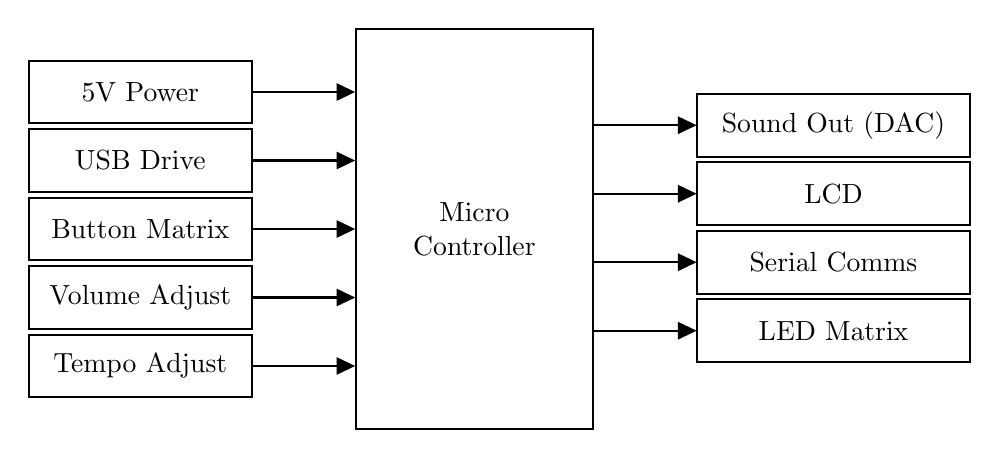
\begin{tikzpicture}[x=0.75pt,y=0.75pt,yscale=-1,xscale=1]
	%uncomment if require: \path (0,431); %set diagram left start at 0, and has height of 431
	
	%Shape: Rectangle [id:dp5381936095328363] 
	\draw   (246.5,62.63) -- (361,62.63) -- (361,255.63) -- (246.5,255.63) -- cycle ;
	%Straight Lines [id:da8765977188339436] 
	\draw    (196.75,93.13) -- (244.25,93.13) ;
	\draw [shift={(246.25,93.13)}, rotate = 180] [fill={rgb, 255:red, 0; green, 0; blue, 0 }  ][line width=0.75]  [draw opacity=0] (8.93,-4.29) -- (0,0) -- (8.93,4.29) -- cycle    ;
	
	%Shape: Rectangle [id:dp36995217586341567] 
	\draw   (89,78) -- (196.5,78) -- (196.5,108.25) -- (89,108.25) -- cycle ;
	%Straight Lines [id:da13737808995401868] 
	\draw    (196.75,126.13) -- (244.25,126.13) ;
	\draw [shift={(246.25,126.13)}, rotate = 180] [fill={rgb, 255:red, 0; green, 0; blue, 0 }  ][line width=0.75]  [draw opacity=0] (8.93,-4.29) -- (0,0) -- (8.93,4.29) -- cycle    ;
	
	%Shape: Rectangle [id:dp07439121123774228] 
	\draw   (89,111) -- (196.5,111) -- (196.5,141.25) -- (89,141.25) -- cycle ;
	%Straight Lines [id:da611957713361752] 
	\draw    (196.75,159.13) -- (244.25,159.13) ;
	\draw [shift={(246.25,159.13)}, rotate = 180] [fill={rgb, 255:red, 0; green, 0; blue, 0 }  ][line width=0.75]  [draw opacity=0] (8.93,-4.29) -- (0,0) -- (8.93,4.29) -- cycle    ;
	
	%Shape: Rectangle [id:dp31809785405688795] 
	\draw   (89,144) -- (196.5,144) -- (196.5,174.25) -- (89,174.25) -- cycle ;
	%Straight Lines [id:da6063583442339884] 
	\draw    (196.75,192.13) -- (244.25,192.13) ;
	\draw [shift={(246.25,192.13)}, rotate = 180] [fill={rgb, 255:red, 0; green, 0; blue, 0 }  ][line width=0.75]  [draw opacity=0] (8.93,-4.29) -- (0,0) -- (8.93,4.29) -- cycle    ;
	
	%Shape: Rectangle [id:dp38581914299250375] 
	\draw   (89,177) -- (196.5,177) -- (196.5,207.25) -- (89,207.25) -- cycle ;
	%Straight Lines [id:da17028430467209366] 
	\draw    (196.75,225.13) -- (244.25,225.13) ;
	\draw [shift={(246.25,225.13)}, rotate = 180] [fill={rgb, 255:red, 0; green, 0; blue, 0 }  ][line width=0.75]  [draw opacity=0] (8.93,-4.29) -- (0,0) -- (8.93,4.29) -- cycle    ;
	
	%Shape: Rectangle [id:dp43755228478774333] 
	\draw   (89,210) -- (196.5,210) -- (196.5,240.25) -- (89,240.25) -- cycle ;
	%Straight Lines [id:da5978587164288591] 
	\draw    (361.25,208.13) -- (408.75,208.13) ;
	\draw [shift={(410.75,208.13)}, rotate = 180] [fill={rgb, 255:red, 0; green, 0; blue, 0 }  ][line width=0.75]  [draw opacity=0] (8.93,-4.29) -- (0,0) -- (8.93,4.29) -- cycle    ;
	
	%Shape: Rectangle [id:dp666439994381903] 
	\draw   (411,193) -- (542.5,193) -- (542.5,223.25) -- (411,223.25) -- cycle ;
	%Straight Lines [id:da49748203015790193] 
	\draw    (361.25,175.13) -- (408.75,175.13) ;
	\draw [shift={(410.75,175.13)}, rotate = 180] [fill={rgb, 255:red, 0; green, 0; blue, 0 }  ][line width=0.75]  [draw opacity=0] (8.93,-4.29) -- (0,0) -- (8.93,4.29) -- cycle    ;
	
	%Shape: Rectangle [id:dp12510077494562744] 
	\draw   (411,160) -- (542.5,160) -- (542.5,190.25) -- (411,190.25) -- cycle ;
	%Straight Lines [id:da15981849232064427] 
	\draw    (361.25,142.13) -- (408.75,142.13) ;
	\draw [shift={(410.75,142.13)}, rotate = 180] [fill={rgb, 255:red, 0; green, 0; blue, 0 }  ][line width=0.75]  [draw opacity=0] (8.93,-4.29) -- (0,0) -- (8.93,4.29) -- cycle    ;
	
	%Shape: Rectangle [id:dp7840394979128142] 
	\draw   (411,127) -- (542.5,127) -- (542.5,157.25) -- (411,157.25) -- cycle ;
	%Straight Lines [id:da3639174829910561] 
	\draw    (361.25,109.13) -- (408.75,109.13) ;
	\draw [shift={(410.75,109.13)}, rotate = 180] [fill={rgb, 255:red, 0; green, 0; blue, 0 }  ][line width=0.75]  [draw opacity=0] (8.93,-4.29) -- (0,0) -- (8.93,4.29) -- cycle    ;
	
	%Shape: Rectangle [id:dp23058766956136134] 
	\draw   (411,94) -- (542.5,94) -- (542.5,124.25) -- (411,124.25) -- cycle ;
	
	% Text Node
	\draw (303.75,159.13) node  [align=center] {Micro\\Controller};
	% Text Node
	\draw (142.75,93.13) node  [align=left] {5V Power};
	% Text Node
	\draw (142.75,126.13) node  [align=left] {USB Drive};
	% Text Node
	\draw (142.75,159.13) node  [align=left] {Button Matrix};
	% Text Node
	\draw (142.75,192.13) node  [align=left] {Volume Adjust};
	% Text Node
	\draw (142.75,225.13) node  [align=left] {Tempo Adjust};
	% Text Node
	\draw (476.75,208.13) node  [align=left] {LED Matrix};
	% Text Node
	\draw (476.75,175.13) node  [align=left] {Serial Comms};
	% Text Node
	\draw (476.75,142.13) node  [align=left] {LCD};
	% Text Node
	\draw (476.75,109.13) node  [align=left] {Sound Out (DAC)};
	
	
	\end{tikzpicture}
\caption{A Basic System Diagram}
\label{fig:basisSysDiag}
\end{figure}\\
Figure \ref{fig:basisSysDiag} shows a basic system diagram based on the project aims. Each of the components in this figure will be explored further in this chapter. There will also be a detailed final system diagram at the end of the chapter.
\section{Button and LED Matrix}
Being the main way for the user to interact with the drum machine, the button and \ac{led} matrices are integral to the correct usage of the device. Many \acap{led} and buttons have to be driven for the interaction to be usable, however, this requires a better understanding of how the matrices are to be set up.
\subsection{Chosen Beat Matrix Design} 
For the physical drum machine, the same technique from Section \ref{sec:beatmatrix} is used. \acap{led} are used as indicators and thus need to be placed in a matrix. Similarly, to change the states of the grid elements, a matrix of buttons will be used. A design of sixteen beats (columns) was chosen with five different sounds (rows). This gives us a matrix of 16 by 5, hence 80 buttons and 80 \acap{led}. These values were chosen by assuming 4 beats in a bar and four bars, hence 16 beats. The number of different sounds, or rows, was determined by spatial restrictions for the \ac{pcb} \cite{pcbguidelines} as well as determining the maximum number of audio files that the \ac{uc} can handle simultaneously.
\subsection{Viable techniques to reduce pin count} \label{sec:pincountReduc}
The problem posed by having, in this case, 80 buttons and 80 \acap{led} is that driving all those would require at least 21 pins on the \ac{uc} for each if it is being multiplexed. This is unrealistic and thus a method must be used to reduce the pin count required to drive the two features.
\subsubsection{Basic Driving}
As mentioned above, it is not viable to connect each node to a pair of pins individually as \acap{uc} generally do not offer that many pins. As there are 80 nodes, there would have to be up to 320 pins to connect the 160 buttons and \acap{led}.\\
An alternative method is to consider the matrix as a set of buttons or \acap{led} at a certain row and column. Using this idea one can drive one of the columns or rows and read or write states on the alternate to select a certain button or \ac{led}. This technique is referred to as single multiplexing \cite{singleMultiplex}. The downside of this technique is that only one row or column of buttons or \acap{led} can be selected at one time, thus the system will need to cycle through the columns or rows respectively. This technique uses the same amount of pins as there are columns and rows, thus 42 pins for all the buttons and \acap{led}. This amount is still too high and should be reduced to make it more viable.
\subsubsection{Driving a Row} \label{sec:rowDriver}
A technique that can be used to reduce pins even further is to drive the columns of the matrix using a separate \ac{ic}. There are three \acap{ic} that can be used to achieve this: Shift Registers, Decoders, and Decade Counters \cite{openMusicLabsAll}. 
\begin{table}[htbp]
	\centering
	\begin{tabular}{|p{2.45cm}|p{1.55cm}|p{1.7cm}|p{2.7cm}|p{2.8cm}|p{2.2cm}|}
		\hline
		\textbf{\ac{ic} Type} & \textbf{Signal Type} & \textbf{Input pins} & \textbf{Simultaneous Outputs (Max)} & \textbf{Extra logic for extension required} & \textbf{Reversed versions available} \\
		\hline
		\aca{sipo} \newline Shift Register & Serial & 3 & $n^*$ & \ding{55} & \ding{51} (\aca{piso})\\
		\hline
		Decade Counter & Serial & 2 & 1 & \ding{51} (AND Gate) & \ding{55} \\
		\hline
		Decoder & Parallel & $\log_2(n^*) $ & 1 & \ding{51} (NOT Gate / Decoder) & \ding{51} \newline (Encoder) \\
		\hline
	\end{tabular}
	\caption{Input Pin Reduction Techniques using \acap{ic}}
	\label{tab:pinreduc}%
\end{table}\\
* - Note that in Table \ref{tab:pinreduc} the value $n$ refers to the number of columns.\\
\textbf{\ac{sipo} Shift Registers} can be used to take in a serial, clock, and possibly a latch signal \cite{srOpenMusic}. As the name implies the chip will take in serial and output a parallel signal. The chip can be driven with a high level on the first clock pulse and a low for all that follows. Each subsequent clock cycle will then shift the signal up one pin on the output side of the \ac{ic}. Alternatively, a serial signal can be shifted through and latched at the end to select multiple columns simultaneously. To extend the number of parallel output pins one can make use of the inverted final output pin to use as the serial pin for consequent matching \ac{ic} \cite{srOpenMusic}.\\
\textbf{Decoders} are the simplest to understand as they set the pin high which corresponds to the binary bits being input \cite{decoderOpenMusic, DecoderMuxAoE}. The downside of this is that only one column can be selected at a time and that the column must be selected manually through serial. A decoder \ac{ic} can be extended to have a greater number of outputs by using a NOT gate or further decoders to split the binary value between \acap{ic} as shown in Figure \ref{fig:decoderentend} \cite{extendDecoder}. 
\begin{figure}[h!]
	\centering
	\begin{subfigure}[b]{0.45\textwidth}
		\centering
		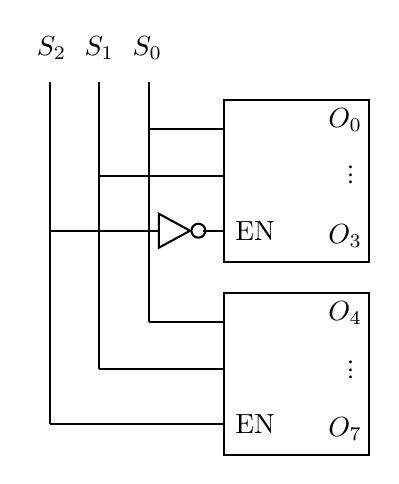
\begin{tikzpicture}[x=0.75pt,y=0.75pt,yscale=-1,xscale=1]
		%uncomment if require: \path (0,268.5); %set diagram left start at 0, and has height of 268.5
		
		%Straight Lines [id:da4685535675893642] 
		\draw    (224,60) -- (224,83) ;
		
		
		%Shape: Rectangle [id:dp028807811878851064] 
		\draw   (260,69) -- (330,69) -- (330,147) -- (260,147) -- cycle ;
		%Straight Lines [id:da2437761404158052] 
		\draw    (224,83) -- (260.25,83) ;
		
		
		%Straight Lines [id:da7464323580851737] 
		\draw    (200,60) -- (200,105.67) ;
		
		
		%Straight Lines [id:da12188935979416193] 
		\draw    (200,105.67) -- (259.67,105.67) ;
		
		
		%Shape: Triangle [id:dp6449692719122406] 
		\draw   (243.67,131.83) -- (228.67,140) -- (228.67,123.67) -- cycle ;
		%Straight Lines [id:da947028663721593] 
		\draw    (250.02,131.83) -- (259.67,131.83) ;
		
		\draw [shift={(247.67,131.83)}, rotate = 0] [color={rgb, 255:red, 0; green, 0; blue, 0 }  ][line width=0.75]      (0, 0) circle [x radius= 3.35, y radius= 3.35]   ;
		%Straight Lines [id:da07881926640580939] 
		\draw    (176,60) -- (176,131.83) ;
		
		
		%Straight Lines [id:da7426941547489794] 
		\draw    (176,131.83) -- (228.67,131.83) ;
		
		
		%Straight Lines [id:da23160509976933286] 
		\draw    (224,83) -- (224,176) ;
		
		
		%Shape: Rectangle [id:dp7426084387946623] 
		\draw   (260,162) -- (330,162) -- (330,240) -- (260,240) -- cycle ;
		%Straight Lines [id:da3166982923913777] 
		\draw    (224,176) -- (260.25,176) ;
		
		
		%Straight Lines [id:da9194338342218067] 
		\draw    (200,105.67) -- (200,198.67) ;
		
		
		%Straight Lines [id:da14845056666605383] 
		\draw    (200,198.67) -- (259.67,198.67) ;
		
		
		%Straight Lines [id:da1995139405507076] 
		\draw    (176,131.83) -- (176,224.83) ;
		
		
		%Straight Lines [id:da8862242231207325] 
		\draw    (176,224.83) -- (260,224.83) ;
		
		
		
		% Text Node
		\draw (275,132) node  [align=left] {EN};
		% Text Node
		\draw (200,44) node   {$S_{2} \ \ S_{1} \ \ S_{0}$};
		% Text Node
		\draw (318.4,78.4) node   {$O_{0}$};
		% Text Node
		\draw (318.4,134.4) node   {$O_{3}$};
		% Text Node
		\draw (275,225) node  [align=left] {EN};
		% Text Node
		\draw (318.4,171.4) node   {$O_{4}$};
		% Text Node
		\draw (318.4,227.4) node   {$O_{7}$};
		% Text Node
		\draw (321,105) node [rotate=-90] [align=left] {...};
		% Text Node
		\draw (321,199) node [rotate=-90] [align=left] {...};
		
		\end{tikzpicture}
		\caption{Using NOT Gate}
	\end{subfigure}
	\hfill
	\begin{subfigure}[b]{0.45\textwidth}
		\centering
		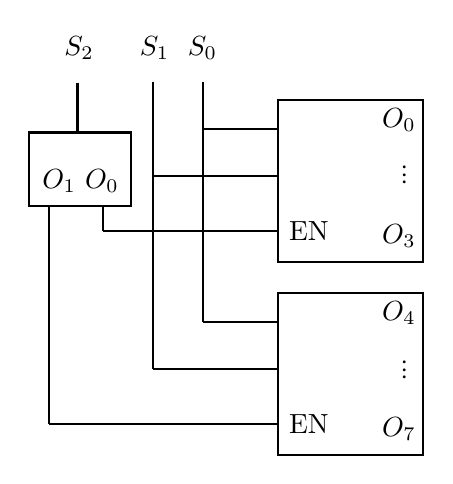
\begin{tikzpicture}[x=0.75pt,y=0.75pt,yscale=-1,xscale=1]
		%uncomment if require: \path (0,268.5); %set diagram left start at 0, and has height of 268.5
		
		%Straight Lines [id:da9281151118799162] 
		\draw    (224,60) -- (224,83) ;
		
		
		%Shape: Rectangle [id:dp569843458366222] 
		\draw   (260,69) -- (330,69) -- (330,147) -- (260,147) -- cycle ;
		%Straight Lines [id:da6131871792028578] 
		\draw    (224,83) -- (260.25,83) ;
		
		
		%Straight Lines [id:da6871028705452948] 
		\draw    (200,60) -- (200,105.67) ;
		
		
		%Straight Lines [id:da21042919473715327] 
		\draw    (200,105.67) -- (259.67,105.67) ;
		
		
		%Straight Lines [id:da5256232936717646] 
		\draw    (176,131.83) -- (260.5,131.83) ;
		
		
		%Straight Lines [id:da3487382006257085] 
		\draw    (224,83) -- (224,176) ;
		
		
		%Shape: Rectangle [id:dp1839932132635731] 
		\draw   (260,162) -- (330,162) -- (330,240) -- (260,240) -- cycle ;
		%Straight Lines [id:da05535190946730606] 
		\draw    (224,176) -- (260.25,176) ;
		
		
		%Straight Lines [id:da8746608490336203] 
		\draw    (200,105.67) -- (200,198.67) ;
		
		
		%Straight Lines [id:da2337980168377387] 
		\draw    (200,198.67) -- (259.67,198.67) ;
		
		
		%Straight Lines [id:da428229538280674] 
		\draw    (149.75,224.83) -- (260,224.83) ;
		
		
		%Shape: Rectangle [id:dp6716362086846552] 
		\draw   (140,84.5) -- (189.5,84.5) -- (189.5,120) -- (140,120) -- cycle ;
		%Straight Lines [id:da5396798017060367] 
		\draw    (163.5,60.5) -- (163.5,84.2) ;
		
		
		%Straight Lines [id:da1506893256268247] 
		\draw    (176,131.83) -- (176,119.38) ;
		
		
		%Straight Lines [id:da8697656801026394] 
		\draw    (149.75,120.38) -- (149.75,224.83) ;
		
		
		
		% Text Node
		\draw (275,132) node  [align=left] {EN};
		% Text Node
		\draw (194,44) node   {$S_{2} \ \ \ \ \ S_{1} \ \ S_{0}$};
		% Text Node
		\draw (318.4,78.4) node   {$O_{0}$};
		% Text Node
		\draw (318.4,134.4) node   {$O_{3}$};
		% Text Node
		\draw (275,225) node  [align=left] {EN};
		% Text Node
		\draw (318.4,171.4) node   {$O_{4}$};
		% Text Node
		\draw (318.4,227.4) node   {$O_{7}$};
		% Text Node
		\draw (321,105) node [rotate=-90] [align=left] {...};
		% Text Node
		\draw (321,199) node [rotate=-90] [align=left] {...};
		% Text Node
		\draw (165,108) node   {$O_{1} \ O_{0}$};
		
		
		\end{tikzpicture}
	\caption{Using 1:2 Decoder}	
\end{subfigure}
	\caption{Extending Decoder \acap{ic} Schematics \cite{extendDecoder}}
	\label{fig:decoderentend}
\end{figure}\\
\textbf{Decade Counters} shift a high bit along with the output pins at every clock cycle \cite{CountersAoE}. This allows for one column to be selected at a time with the knowledge that the next column will be selected at the next clock cycle. Decade counters too can have the number of outputs extended, however, this requires AND gates as can be seen in Figure \ref{fig:extenddc}. This setup causes the first counter to stop whilst the second is active and vice versa \cite{chainingCounters}. A notable issue would be that some outputs, such as the first pin on the 2nd chip, are no longer correct or usable and the whole system is shifted. Thankfully the system still only requires two input signals, the clock and reset lines, regardless of how large the loop becomes.
\begin{figure}[h!]
	\centering
	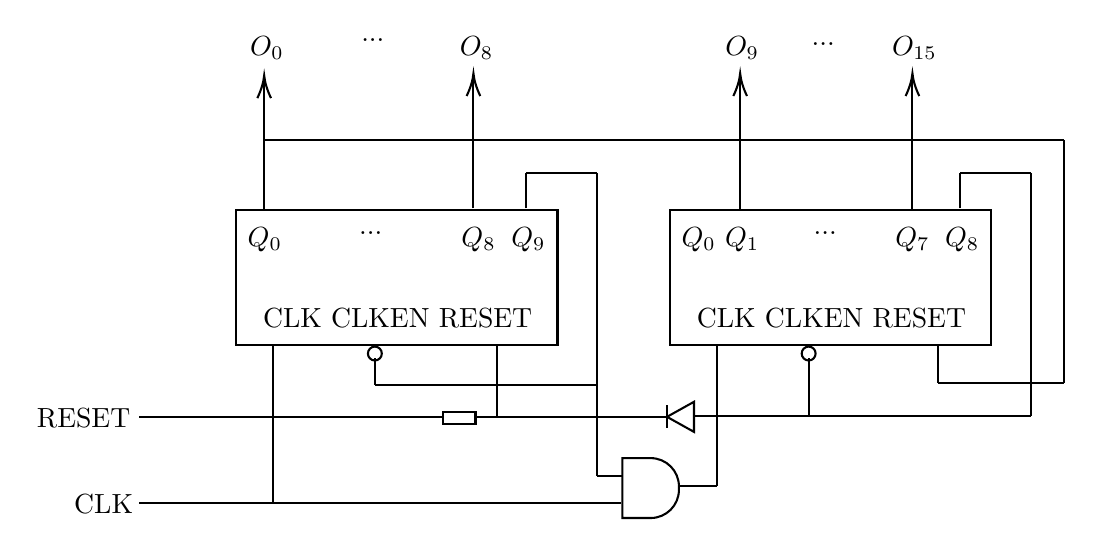
\begin{tikzpicture}[x=0.75pt,y=0.75pt,yscale=-1,xscale=1]
	%uncomment if require: \path (0,370); %set diagram left start at 0, and has height of 370
	
	%Shape: Rectangle [id:dp671023169283194] 
	\draw   (127,175) -- (282,175) -- (282,240) -- (127,240) -- cycle ;
	%Straight Lines [id:da36789801103934505] 
	\draw    (267,174) -- (267,157) ;
	
	
	%Straight Lines [id:da9283663831953444] 
	\draw    (267,157) -- (301,157) ;
	
	
	%Straight Lines [id:da29725876431210474] 
	\draw    (301,157) -- (301,259) ;
	
	
	%Straight Lines [id:da9630025146963983] 
	\draw    (194,259) -- (301,259) ;
	
	
	%Straight Lines [id:da5673404807383264] 
	\draw    (194,246.35) -- (194,259) ;
	
	\draw [shift={(194,244)}, rotate = 90] [color={rgb, 255:red, 0; green, 0; blue, 0 }  ][line width=0.75]      (0, 0) circle [x radius= 3.35, y radius= 3.35]   ;
	%Shape: Rectangle [id:dp14245439224132106] 
	\draw   (336,175) -- (491,175) -- (491,240) -- (336,240) -- cycle ;
	%Straight Lines [id:da5890739685934039] 
	\draw    (476,174) -- (476,157) ;
	
	
	%Straight Lines [id:da25504052077375894] 
	\draw    (476,157) -- (510,157) ;
	
	
	%Straight Lines [id:da10741148003014156] 
	\draw    (510,157) -- (510,274) ;
	
	
	%Straight Lines [id:da17697316011473796] 
	\draw    (403,274) -- (510,274) ;
	
	
	%Straight Lines [id:da8705689799622696] 
	\draw    (403,246.35) -- (403,274) ;
	
	\draw [shift={(403,244)}, rotate = 90] [color={rgb, 255:red, 0; green, 0; blue, 0 }  ][line width=0.75]      (0, 0) circle [x radius= 3.35, y radius= 3.35]   ;
	%Straight Lines [id:da2223372943251709] 
	\draw    (403,274) -- (347.5,274) ;
	
	
	%Shape: Triangle [id:dp0036163693791919638] 
	\draw   (334.75,274.5) -- (347.75,267.25) -- (347.75,281.75) -- cycle ;
	%Straight Lines [id:da4132789132766448] 
	\draw    (252.75,274.5) -- (334.75,274.5) ;
	\draw [shift={(334.75,274.5)}, rotate = 180] [color={rgb, 255:red, 0; green, 0; blue, 0 }  ][line width=0.75]    (0,5.59) -- (0,-5.59)   ;
	
	%Straight Lines [id:da3053017911756648] 
	\draw    (252.75,239.5) -- (252.75,274.5) ;
	
	
	%Straight Lines [id:da2415533137092909] 
	\draw    (252.75,274.5) -- (242.95,274.5) ;
	
	
	%Shape: Rectangle [id:dp36577683975285025] 
	\draw   (227,272.1) -- (242.5,272.1) -- (242.5,278.1) -- (227,278.1) -- cycle ;
	%Rounded Same Side Corner Rect [id:dp2948546410374566] 
	\draw   (326.88,294.38) .. controls (334.4,294.38) and (340.5,300.48) .. (340.5,308) -- (340.5,309.63) .. controls (340.5,317.15) and (334.4,323.25) .. (326.88,323.25) -- (313.25,323.25) .. controls (313.25,323.25) and (313.25,323.25) .. (313.25,323.25) -- (313.25,294.38) .. controls (313.25,294.38) and (313.25,294.38) .. (313.25,294.38) -- cycle ;
	%Straight Lines [id:da1289297369934561] 
	\draw    (301,259) -- (301,303) ;
	
	
	%Straight Lines [id:da6977063029312365] 
	\draw    (301,303) -- (313.5,303) ;
	
	
	%Straight Lines [id:da26801862689975575] 
	\draw    (312.5,316) -- (80.5,316) ;
	
	
	%Straight Lines [id:da4513157267130872] 
	\draw    (80.5,274.5) -- (226.95,274.5) ;
	
	
	%Straight Lines [id:da491579941616326] 
	\draw    (144.8,239.8) -- (144.8,315.4) ;
	
	
	%Straight Lines [id:da9583496669840117] 
	\draw    (340.5,308) -- (358.67,308) ;
	
	
	%Straight Lines [id:da02355792053266259] 
	\draw    (358.67,308) -- (358.67,239.33) ;
	
	
	%Straight Lines [id:da41105514252013076] 
	\draw    (140.67,175) -- (140.67,141) ;
	
	
	%Straight Lines [id:da40872784052262334] 
	\draw    (140.67,141) -- (526,141) ;
	
	
	%Straight Lines [id:da06139958242679655] 
	\draw    (526,141) -- (526,258) ;
	
	
	%Straight Lines [id:da15992891793043795] 
	\draw    (526,258) -- (465.33,258) ;
	
	
	%Straight Lines [id:da05792403432120952] 
	\draw    (465.33,258) -- (465.33,239.33) ;
	
	
	%Straight Lines [id:da6092695180887999] 
	\draw    (140.67,141) -- (140.67,112) ;
	\draw [shift={(140.67,110)}, rotate = 450] [color={rgb, 255:red, 0; green, 0; blue, 0 }  ][line width=0.75]    (10.93,-3.29) .. controls (6.95,-1.4) and (3.31,-0.3) .. (0,0) .. controls (3.31,0.3) and (6.95,1.4) .. (10.93,3.29)   ;
	
	%Straight Lines [id:da30314532933003613] 
	\draw    (241.5,174) -- (241.5,111) ;
	\draw [shift={(241.5,109)}, rotate = 450] [color={rgb, 255:red, 0; green, 0; blue, 0 }  ][line width=0.75]    (10.93,-3.29) .. controls (6.95,-1.4) and (3.31,-0.3) .. (0,0) .. controls (3.31,0.3) and (6.95,1.4) .. (10.93,3.29)   ;
	
	%Straight Lines [id:da7261945480656935] 
	\draw    (370,175) -- (370,111) ;
	\draw [shift={(370,109)}, rotate = 450] [color={rgb, 255:red, 0; green, 0; blue, 0 }  ][line width=0.75]    (10.93,-3.29) .. controls (6.95,-1.4) and (3.31,-0.3) .. (0,0) .. controls (3.31,0.3) and (6.95,1.4) .. (10.93,3.29)   ;
	
	%Straight Lines [id:da9644050934958703] 
	\draw    (453,175) -- (453,111) ;
	\draw [shift={(453,109)}, rotate = 450] [color={rgb, 255:red, 0; green, 0; blue, 0 }  ][line width=0.75]    (10.93,-3.29) .. controls (6.95,-1.4) and (3.31,-0.3) .. (0,0) .. controls (3.31,0.3) and (6.95,1.4) .. (10.93,3.29)   ;
	
	
	% Text Node
	\draw (205,227) node  [align=left] {CLK CLKEN RESET};
	% Text Node
	\draw (141,189) node   {$Q_{0}$};
	% Text Node
	\draw (244,189) node   {$Q_{8}$};
	% Text Node
	\draw (268,189) node   {$Q_{9}$};
	% Text Node
	\draw (192,186) node  [align=left] {...};
	% Text Node
	\draw (414,227) node  [align=left] {CLK CLKEN RESET};
	% Text Node
	\draw (350,189) node   {$Q_{0}$};
	% Text Node
	\draw (453,189) node   {$Q_{7}$};
	% Text Node
	\draw (477,189) node   {$Q_{8}$};
	% Text Node
	\draw (411,186) node  [align=left] {...};
	% Text Node
	\draw (63.33,316.33) node  [align=left] {CLK};
	% Text Node
	\draw (53.67,275) node  [align=left] {RESET};
	% Text Node
	\draw (371,189) node   {$Q_{1}$};
	% Text Node
	\draw (142,97) node   {$O_{0}$};
	% Text Node
	\draw (243,97) node   {$O_{8}$};
	% Text Node
	\draw (371,97) node   {$O_{9}$};
	% Text Node
	\draw (454,97) node   {$O_{15}$};
	% Text Node
	\draw (193,93) node  [align=left] {...};
	% Text Node
	\draw (410,95) node  [align=left] {...};
	
	
	\end{tikzpicture}
	\caption{Extending Decade Counter \acap{ic} Schematic \cite{chainingCounters}}
	\label{fig:extenddc}
\end{figure}

\subsubsection{Input}
It can prove useful to drive large amounts of pins with very few connections to a controller, as in Section \ref{sec:rowDriver}, but equally useful is reading the current state of a large number of pins and encoding this in a way for a controller to understand. A column in Table \ref{tab:pinreduc} shows that two of the circuits can also execute this task if an alternate version of the respective \ac{ic} is used. For the \ac{sipo} shift register, a \ac{piso} shift register can do the inverse job: taking in a large number of parallel pins and outputting a serial signal \cite{PISOsrOpenMusic}. Similarly, a decoder acts in the opposite way of an encoder. The encoder will take a parallel signal and convert it to the respective binary value \cite{encoderExplan}. These two \acap{ic} are not the only options for reducing the number of pins to read a large number of input states, another is a \ac{mux}. The \ac{mux} design would require the \ac{uc} to step through each binary value on the select pins of the \ac{mux} and check if the output pin's state has changed \cite{DecoderMuxAoE}. This technique is however rather redundant as an encoder essentially is being designed with the \ac{mux}, just with one extra pin.\\
\begin{table}[h!]
	\centering
	\begin{tabular}{|p{3.9cm}|p{2.15cm}|p{2.15cm}|p{4cm}|}
		\hline 
		\textbf{IC Type} & \multicolumn{2}{c|}{\textbf{\textnumero \ Connections to \ac{uc}}}& \textbf{Max Simultaneous} \\ 
		& \multicolumn{1}{l}{\textbf{Control}} & \textbf{Data} & \textbf{inputs} \\
		\hline 
		\ac{piso} Shift Register & 3 & 1 & $n$ \\ 
		\hline 
		Encoder & 0 & $\log_2(n)$ & 1 \\ 
		\hline 
		Multiplexer & $\log_2(n)$ & 1 & 1 \\ 
		\hline 
		Direct Connection & 0 & $n$ & $n$ \\ 
		\hline 
	\end{tabular} 
	\caption{Input Pin Reduction Methods}
	\label{tab:inputpinreduc}
\end{table}\\
Table \ref{tab:inputpinreduc} shows the number of pins required to control various techniques of reducing pin count for reading a large number of pin states as well as the number of connections needed to read the data value. The number of input states, $n$, that the technique can read simultaneously is also listed, this is equivalent to how many pins of the parallel input can be high at the same time.
\begin{figure}[h!]
	\centering
	\begin{tikzpicture}[scale = 1.1]
	\begin{axis}[
	axis lines = left,
	xlabel = Data Inputs ($n$),
	ylabel = {\textnumero  \  Connections to \ac{uc}},
	grid = major,
	legend pos = north west,
	xtick = {1,2,3,4,5,6,7,8},
	ytick = {1,2,3,4,5,6,7,8},
	legend entries = {PISO Shift Register, Encoder, Multiplexer, Direct Connection},
	]
	\addlegendimage{mark = square, red}
	\addlegendimage{mark = triangle, blue}
	\addlegendimage{mark = diamond, teal}
	\addlegendimage{mark = o, magenta}
	
	%Below the red parabola is defined
	\addplot [
	domain=1:8, 
	samples=8, 
	color=red,
	thick,
	mark = square,
	]
	{4};
	%\addlegendentry{PISO Shift Register}
	
	%Here the blue parabloa is defined
	\addplot [
	domain=2:8, 
	samples=100, 
	color=blue,
	thick,
	]
	{log2(x)};
	%\addlegendentry{Encoder}
	\addplot [
	domain=2:8, 
	samples=7, 
	color=blue,
	thick,
	mark = triangle,
	only marks,
	]
	{ceil(log2(x))};
	
	\addplot [
	domain=2:8, 
	samples=100, 
	color=teal,
	thick,
	style = solid,
	]
	{log2(x)+1};
	%\addlegendentry{Multiplexer}
	
	\addplot [
	domain=2:8, 
	samples=7, 
	color=teal,
	thick,
	%style = dashed,
	mark = diamond,
	only marks,
	]
	{ceil(log2(x)+1)};
	
	\addplot [
	domain=1:8, 
	samples=8, 
	color=magenta,
	thick,
	mark = o,
	]
	{x};

	%\addlegendentry{Direct Connection}
	
	\end{axis}
\end{tikzpicture}
\caption{\textnumero \  of connections to the \ac{uc} for Input Pin Reduction}	
\label{fig:ioUCCons}
\end{figure}\\
Figure \ref{fig:ioUCCons} shows the graphs of each technique's number of data inputs to a number of connections required to the \ac{uc}. The data for this figure comes from Table \ref{tab:inputpinreduc}. The lines for the Encoder (dark blue) and the Multiplexer (teal) are indicated differently to the other lines. The marker of the matching colour shows the actual value of needed connections to the \ac{uc} for every given number of inputs. This is done as there cannot be a fraction of a pin used, thus the ceiling of the formula is used here. For example, if using an encoder with 3 data inputs $\log_2 (3) = 1.58$, this is not a valid number of connections to the \ac{uc}, thus this will need to be rounded up to two, as is shown in the figure. It should also be noted that these two techniques only begin at two data inputs as a 1 to 1 encoder or \ac{mux} would simply be a short circuit.\\
Consulting Table \ref{tab:inputpinreduc} and Figure \ref{fig:ioUCCons}, it can be seen that if the more than one high data state can be expected simultaneously the direct connection method proves the most efficient up until 4 data inputs. After this point the \ac{piso} Shift Register set-up will be more efficient. Alternatively, if only one high data state is expected at a time, the Encoder set-up will always prove one pin on the \ac{uc} more efficient, as explained before.\\
Techniques to expand the number of data input pins over multiple \acap{ic} will not be discussed as for this project it will not prove necessary. There are five rows, which falls under the eight-pin input of most \acap{ic}, hence this does not need to be looked into more.
\subsubsection{Driving Rows and Columns as a chain}
If no data needs to be received back by the \ac{uc} both rows and columns can be controlled by a single chain of \acap{ic} \cite{srOpenMusic}. This technique can be used in the case of the \acap{led} as the positive and negative pins will be set high and low depending on its intended state. Seeing as the \acap{led} require a potential difference to light up there are two methods of turning the \ac{led} off can be used: Firstly driving the positive side of the \ac{led} low to match the low state of the negative pin, or secondly matching the negative pin high to that of the positive pin. Both methods will cause there to be no potential difference over the \ac{led} and thus it will not light.
\subsubsection{Driving Serial Peripherals from the $\mu$C}
Up to this point no technique for driving the clock, serial data and other pins have been mentioned. The simplest one to consider is \ac{spi} as this provides not only a clock signal but also handles the serial data transmission \cite{SPIAoE}. This interface could also be further expanded upon by manually setting \ac{gpio} pins from the \ac{uc} to control \ac{ic} related functions, such as to enable or chip select. An example of a place where this could be used is for a Shift Register. In that case, the Serial Data and RCLK pins are controlled by the \ac{spi} interface and the SRCLK pin will be controlled manually to set the state low before and high after transmission. \\
An alternative technique is 'bit banging' \cite{bitbanging}. This is where software on the \ac{uc} directly controls the states of all the pins as \ac{gpio} pins manually. This would have the \ac{uc} run a loop with a "clock" changing state as well as outputting the corresponding data bit as fast as the \ac{uc} can run the code. This may allow for more control of each signal, but the increased coding complexity and lack of known timing may cause issues for some \acap{ic} \cite{bitbanging}. Overall, this method is not recommended if an alternative, such as \ac{spi}, is available on the \ac{uc} being used.
\subsection{Basic Button and LED connection}
Up until this point buttons and \acap{led} have only been mentioned but no thought has been given as to how they will be connected in the matrix. Thanks to the \ac{led} being a diode it will only allow current to pass in one direction. Using the formation shown in Figure \ref{sfig:ledBasic} it can be determined that to power any given \ac{led} in this matrix its corresponding row must be set high and column set low.\\
For the buttons, it is slightly more complex as now a state of a certain node must be read by the \ac{uc}. The button connections in the matrix can be seen in Figure \ref{sfig:btnBasic}. To achieve this the columns will be driven high one at a time with the rows being pulled low through a resistor. Depressing the button will cause the column to be shorted to the row through a diode. The diode is there so that multiple buttons can be depressed simultaneously, and the state of each can still be read independently. The potential difference on each row can be read by the \ac{uc}. If it is high then the button at the respective row and column is being depressed and vice-versa.
\begin{figure}[h!]
	\centering
	\begin{subfigure}[b]{0.45\textwidth}
		\centering
		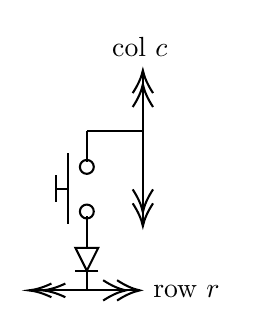
\begin{tikzpicture}[x=0.75pt,y=0.75pt,yscale=-1,xscale=1]
		%uncomment if require: \path (0,204); %set diagram left start at 0, and has height of 204
		
		%Straight Lines [id:da65934185809732] 
		\draw    (77,119) -- (77,132) ;
		
		
		%Straight Lines [id:da11132954370762471] 
		\draw    (77,125.5) -- (83,125.5) ;
		
		
		%Straight Lines [id:da5890963595470742] 
		\draw    (83,108.5) -- (83,142.5) ;
		
		
		%Straight Lines [id:da8803001274966733] 
		\draw    (92,138.85) -- (92,154) ;
		
		\draw [shift={(92,136.5)}, rotate = 90] [color={rgb, 255:red, 0; green, 0; blue, 0 }  ][line width=0.75]      (0, 0) circle [x radius= 3.35, y radius= 3.35]   ;
		%Straight Lines [id:da26652637635730003] 
		\draw    (92,97.5) -- (92,112.65) ;
		\draw [shift={(92,115)}, rotate = 90] [color={rgb, 255:red, 0; green, 0; blue, 0 }  ][line width=0.75]      (0, 0) circle [x radius= 3.35, y radius= 3.35]   ;
		
		%Shape: Triangle [id:dp1516172183109996] 
		\draw   (92,165) -- (86.5,154) -- (97.5,154) -- cycle ;
		%Straight Lines [id:da3332173038583133] 
		\draw    (92,165) -- (92,174.5) ;
		
		\draw [shift={(92,165)}, rotate = 270] [color={rgb, 255:red, 0; green, 0; blue, 0 }  ][line width=0.75]    (0,5.59) -- (0,-5.59)   ;
		%Straight Lines [id:da10862089864488311] 
		\draw    (92,97.5) -- (119,97.5) ;
		
		
		%Straight Lines [id:da6588501488134604] 
		\draw    (64,174.5) -- (117.5,174.5) ;
		\draw [shift={(117.5,174.5)}, rotate = 180] [color={rgb, 255:red, 0; green, 0; blue, 0 }  ][line width=0.75]    (17.64,-4.9) .. controls (13.66,-2.3) and (10.02,-0.67) .. (6.71,0) .. controls (10.02,0.67) and (13.66,2.3) .. (17.64,4.9)(10.93,-4.9) .. controls (6.95,-2.3) and (3.31,-0.67) .. (0,0) .. controls (3.31,0.67) and (6.95,2.3) .. (10.93,4.9)   ;
		\draw [shift={(64,174.5)}, rotate = 0] [color={rgb, 255:red, 0; green, 0; blue, 0 }  ][line width=0.75]    (17.64,-3.29) .. controls (13.66,-1.4) and (10.02,-0.3) .. (6.71,0) .. controls (10.02,0.3) and (13.66,1.4) .. (17.64,3.29)(10.93,-3.29) .. controls (6.95,-1.4) and (3.31,-0.3) .. (0,0) .. controls (3.31,0.3) and (6.95,1.4) .. (10.93,3.29)   ;
		%Straight Lines [id:da4301295332879802] 
		\draw    (119,68.5) -- (119,143.5) ;
		\draw [shift={(119,143.5)}, rotate = 270] [color={rgb, 255:red, 0; green, 0; blue, 0 }  ][line width=0.75]    (17.64,-4.9) .. controls (13.66,-2.3) and (10.02,-0.67) .. (6.71,0) .. controls (10.02,0.67) and (13.66,2.3) .. (17.64,4.9)(10.93,-4.9) .. controls (6.95,-2.3) and (3.31,-0.67) .. (0,0) .. controls (3.31,0.67) and (6.95,2.3) .. (10.93,4.9)   ;
		\draw [shift={(119,68.5)}, rotate = 90] [color={rgb, 255:red, 0; green, 0; blue, 0 }  ][line width=0.75]    (17.64,-4.9) .. controls (13.66,-2.3) and (10.02,-0.67) .. (6.71,0) .. controls (10.02,0.67) and (13.66,2.3) .. (17.64,4.9)(10.93,-4.9) .. controls (6.95,-2.3) and (3.31,-0.67) .. (0,0) .. controls (3.31,0.67) and (6.95,2.3) .. (10.93,4.9)   ;
		
		% Text Node
		\draw (140,175) node  [align=left] {row $\displaystyle r$};
		% Text Node
		\draw (117.5,57) node  [align=left] {col $\displaystyle c$};
		
		
		\end{tikzpicture}
		\caption{Button Connection \cite{singleMultiplex}}
		\label{sfig:btnBasic}
	\end{subfigure}
	\hfill
	\begin{subfigure}[b]{0.45\textwidth}
		\centering
		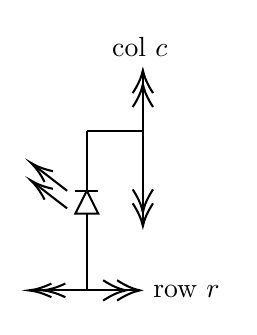
\begin{tikzpicture}[x=0.75pt,y=0.75pt,yscale=-1,xscale=1]
		%uncomment if require: \path (0,300); %set diagram left start at 0, and has height of 300
		
		%Shape: Triangle [id:dp09939159071014059] 
		\draw   (112,146.5) -- (117.5,157.5) -- (106.5,157.5) -- cycle ;
		%Straight Lines [id:da5940981398616236] 
		\draw    (112,146.5) -- (112,117.5) ;
		
		\draw [shift={(112,146.5)}, rotate = 450] [color={rgb, 255:red, 0; green, 0; blue, 0 }  ][line width=0.75]    (0,5.59) -- (0,-5.59)   ;
		%Straight Lines [id:da5490022962553698] 
		\draw    (112,117.5) -- (139,117.5) ;
		
		
		%Straight Lines [id:da5840538149227372] 
		\draw    (84,194.5) -- (137.5,194.5) ;
		\draw [shift={(137.5,194.5)}, rotate = 180] [color={rgb, 255:red, 0; green, 0; blue, 0 }  ][line width=0.75]    (17.64,-4.9) .. controls (13.66,-2.3) and (10.02,-0.67) .. (6.71,0) .. controls (10.02,0.67) and (13.66,2.3) .. (17.64,4.9)(10.93,-4.9) .. controls (6.95,-2.3) and (3.31,-0.67) .. (0,0) .. controls (3.31,0.67) and (6.95,2.3) .. (10.93,4.9)   ;
		\draw [shift={(84,194.5)}, rotate = 0] [color={rgb, 255:red, 0; green, 0; blue, 0 }  ][line width=0.75]    (17.64,-3.29) .. controls (13.66,-1.4) and (10.02,-0.3) .. (6.71,0) .. controls (10.02,0.3) and (13.66,1.4) .. (17.64,3.29)(10.93,-3.29) .. controls (6.95,-1.4) and (3.31,-0.3) .. (0,0) .. controls (3.31,0.3) and (6.95,1.4) .. (10.93,3.29)   ;
		%Straight Lines [id:da5691400211012667] 
		\draw    (139,88.5) -- (139,163.5) ;
		\draw [shift={(139,163.5)}, rotate = 270] [color={rgb, 255:red, 0; green, 0; blue, 0 }  ][line width=0.75]    (17.64,-4.9) .. controls (13.66,-2.3) and (10.02,-0.67) .. (6.71,0) .. controls (10.02,0.67) and (13.66,2.3) .. (17.64,4.9)(10.93,-4.9) .. controls (6.95,-2.3) and (3.31,-0.67) .. (0,0) .. controls (3.31,0.67) and (6.95,2.3) .. (10.93,4.9)   ;
		\draw [shift={(139,88.5)}, rotate = 90] [color={rgb, 255:red, 0; green, 0; blue, 0 }  ][line width=0.75]    (17.64,-4.9) .. controls (13.66,-2.3) and (10.02,-0.67) .. (6.71,0) .. controls (10.02,0.67) and (13.66,2.3) .. (17.64,4.9)(10.93,-4.9) .. controls (6.95,-2.3) and (3.31,-0.67) .. (0,0) .. controls (3.31,0.67) and (6.95,2.3) .. (10.93,4.9)   ;
		%Straight Lines [id:da7146749708886269] 
		\draw    (112,157.5) -- (112,195) ;
		
		
		%Straight Lines [id:da017921802419498034] 
		\draw    (102.5,146.5) -- (86.58,134.22) ;
		\draw [shift={(85,133)}, rotate = 397.65] [color={rgb, 255:red, 0; green, 0; blue, 0 }  ][line width=0.75]    (10.93,-3.29) .. controls (6.95,-1.4) and (3.31,-0.3) .. (0,0) .. controls (3.31,0.3) and (6.95,1.4) .. (10.93,3.29)   ;
		
		%Straight Lines [id:da2750719795337271] 
		\draw    (102.5,155) -- (86.58,142.72) ;
		\draw [shift={(85,141.5)}, rotate = 397.65] [color={rgb, 255:red, 0; green, 0; blue, 0 }  ][line width=0.75]    (10.93,-3.29) .. controls (6.95,-1.4) and (3.31,-0.3) .. (0,0) .. controls (3.31,0.3) and (6.95,1.4) .. (10.93,3.29)   ;
		
		
		% Text Node
		\draw (160,195) node  [align=left] {row $\displaystyle r$};
		% Text Node
		\draw (137.5,77) node  [align=left] {col $\displaystyle c$};
		
		
		\end{tikzpicture}
		\caption{\ac{led} Connection \cite{ledsTPICC}}	
		\label{sfig:ledBasic}
	\end{subfigure}
	\caption{Basic button and \ac{led} Diagrams}
	\label{fig:btnledBasic}
\end{figure}
\subsection{Chosen Designs}
There are several designs to choose from as discussed in the previous section. Each has its own advantages and disadvantages. Several iterations of chosen designs were made until a final form was reached. These chosen designs will be discussed in the section for buttons and \acap{led} respectively below. 
\subsubsection{Button Matrix Driver}
For the button matrix, two set-ups of connections must be used to drive the rows and columns separately. This is necessary as there has to be a state set for the columns and the respective states must be read back in from the rows.\\
To read in the states from the matrix's rows a technique for five inputs should be considered with the ability to read all five pins simultaneously. Consulting Table \ref{tab:inputpinreduc} and Figure \ref{fig:ioUCCons} the options can be reduced to the \ac{piso} Shift Register or Direct Connection techniques. The most efficient option, in terms of the number of required pins on the \ac{uc}, would be the Shift Registers. This technique could prove more tedious to deal with in software and as another point of failure. The direct connections may use one more pin (five instead of four), but the simplicity that comes with this technique allows for faster response in software on the \ac{uc}. Using the Shift Register technique would also require an additional clock interface which is not available on the \ac{uc} \cite{f411}. For these reasons the direct connection technique is used.\\
To drive the columns the techniques from Table \ref{tab:pinreduc} are considered: Shift Registers, Decade Counters, and Decoders. For this application only one column will be driven at a time thus all the solutions would work. Of the three methods, the decoder would be the most difficult to implement in software as well as requiring the most amount of pins. This method would need $\log_2(16) = 4$ pins, as opposed to the maximum of three which the Shift Register technique requires. Both other techniques require the \ac{uc} to keep track of the currently selected column. This, therefore, leaves the choice between a reduced pin count (two vs three), and the simplicity of controlling and building the circuit. Even though the Decade Counter technique requires a more complicated circuit, as is seen in Figure \ref{fig:extenddc}, it is simpler to control from the software. The Shift Register technique requires the software to trigger the data manually, whereas the decade counter, in its current formation, will step from pin zero through pin fifteen (sixteen pins) and automatically reset. For this reason and the reduced pin count, the decade counter technique is used.\\
The \acap{ic} needed for this design \cite{chainingCountersSelf} are the 74HC4017 Decade Counter \cite{4017}, and 74HC08 AND Gates \cite{7408}. The circuit will need a diode, an FDLL4148 \cite{Diode} is used, and a 1k$\Omega$ resistor. The diode allows the system to be manually reset, without it the clock enable of the second \ac{ic}, and all connected points, will remain near zero Volts, hence never resetting the circuit. The resistor is in place to allow the reset state from the \ac{uc} to pull the value rather than setting the state. This allows the output from the second \ac{ic} to pull the voltage high on the reset pin of the first \ac{ic} as otherwise this would be pinned to low when the reset is low \cite{chainingCountersSelf}.
\subsubsection{LED Matrix Driver} \label{sec:LEDDrvr}
As explained previously, the \ac{led} driver can be made of a single chain of \acap{ic}. In this case, the \acap{ic} would have to be \ac{sipo} Shift Registers as the serial signal has to be passed through the entire system and then maintained there for a short time to light the appropriate \ac{led}. Two methods were considered to drive the columns of the matrix. These would require a method of draining the current generated by, up to, all the rows in said column. The first method made use of the TPIC6C596 \ac{ic} \cite{tpic}. This \ac{ic} allows for up to 100mA of continuous drain current with a peak capability, when pulsed, of 250mA per pin \cite{tpic}. This method would allow the \ac{ic} to slot in the chain of \ac{sipo} Shift Registers, as shown in Figure \ref{sfig:sr596}. The second method makes use of the same Shift Register as used for the rows, to which the ULN2803A Darlington Transistor Array \ac{ic} \cite{uln2803} will be connected on the outputs, as shown in Figure \ref{sfig:sr2803}. This \ac{ic} allows for up to a 500mA collector current to be drained \cite{uln2803}.
\begin{figure}[h!]
	\centering
	\begin{subfigure}[b]{\textwidth}
		\centering
		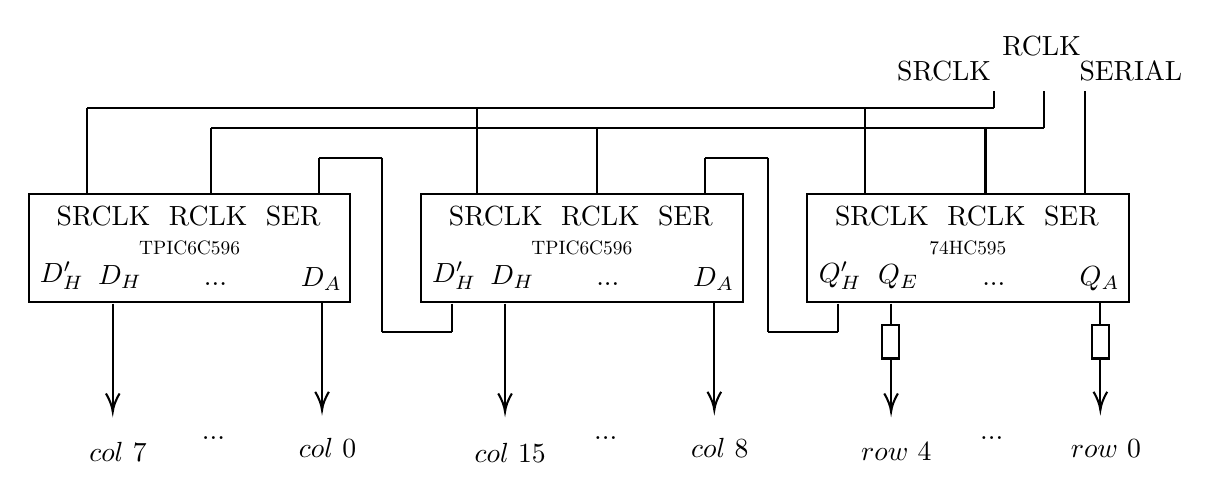
\begin{tikzpicture}[x=0.75pt,y=0.75pt,yscale=-0.8,xscale=1, rotate=90]
		%uncomment if require: \path (0,561); %set diagram left start at 0, and has height of 561
		
		%Shape: Rectangle [id:dp671023169283194] 
		\draw   (199,11) -- (199,166) -- (134,166) -- (134,11) -- cycle ;
		%Straight Lines [id:da36789801103934505] 
		\draw    (200,151) -- (217,151) ;
		
		
		%Straight Lines [id:da9283663831953444] 
		\draw    (217,151) -- (217,185) ;
		
		
		%Straight Lines [id:da41105514252013076] 
		\draw    (199,24.67) -- (233,24.67) ;
		
		
		%Straight Lines [id:da6092695180887999] 
		\draw    (233,24.67) -- (262,24.67) ;
		\draw [shift={(264,24.67)}, rotate = 180] [color={rgb, 255:red, 0; green, 0; blue, 0 }  ][line width=0.75]    (10.93,-3.29) .. controls (6.95,-1.4) and (3.31,-0.3) .. (0,0) .. controls (3.31,0.3) and (6.95,1.4) .. (10.93,3.29)   ;
		
		%Straight Lines [id:da30314532933003613] 
		\draw    (200,125.5) -- (263,125.5) ;
		\draw [shift={(265,125.5)}, rotate = 180] [color={rgb, 255:red, 0; green, 0; blue, 0 }  ][line width=0.75]    (10.93,-3.29) .. controls (6.95,-1.4) and (3.31,-0.3) .. (0,0) .. controls (3.31,0.3) and (6.95,1.4) .. (10.93,3.29)   ;
		
		%Shape: Rectangle [id:dp932788918126821] 
		\draw   (199,197) -- (199,352) -- (134,352) -- (134,197) -- cycle ;
		%Straight Lines [id:da46578914869777743] 
		\draw    (200,337) -- (217,337) ;
		
		
		%Straight Lines [id:da7447653000090828] 
		\draw    (217,337) -- (217,371) ;
		
		
		%Straight Lines [id:da9370935142219265] 
		\draw    (199,210.67) -- (233,210.67) ;
		
		
		%Straight Lines [id:da5226477182035949] 
		\draw    (233,210.67) -- (262,210.67) ;
		\draw [shift={(264,210.67)}, rotate = 180] [color={rgb, 255:red, 0; green, 0; blue, 0 }  ][line width=0.75]    (10.93,-3.29) .. controls (6.95,-1.4) and (3.31,-0.3) .. (0,0) .. controls (3.31,0.3) and (6.95,1.4) .. (10.93,3.29)   ;
		
		%Straight Lines [id:da6377928002897821] 
		\draw    (200,311.5) -- (263,311.5) ;
		\draw [shift={(265,311.5)}, rotate = 180] [color={rgb, 255:red, 0; green, 0; blue, 0 }  ][line width=0.75]    (10.93,-3.29) .. controls (6.95,-1.4) and (3.31,-0.3) .. (0,0) .. controls (3.31,0.3) and (6.95,1.4) .. (10.93,3.29)   ;
		
		%Shape: Rectangle [id:dp9609493905246349] 
		\draw   (199,386) -- (199,541) -- (134,541) -- (134,386) -- cycle ;
		%Straight Lines [id:da17608637763078638] 
		\draw    (199,399.67) -- (233,399.67) ;
		
		
		%Straight Lines [id:da6274994019706419] 
		\draw    (233,399.67) -- (262,399.67) ;
		\draw [shift={(264,399.67)}, rotate = 180] [color={rgb, 255:red, 0; green, 0; blue, 0 }  ][line width=0.75]    (10.93,-3.29) .. controls (6.95,-1.4) and (3.31,-0.3) .. (0,0) .. controls (3.31,0.3) and (6.95,1.4) .. (10.93,3.29)   ;
		
		%Straight Lines [id:da2120918910874514] 
		\draw    (200,500.5) -- (263,500.5) ;
		\draw [shift={(265,500.5)}, rotate = 180] [color={rgb, 255:red, 0; green, 0; blue, 0 }  ][line width=0.75]    (10.93,-3.29) .. controls (6.95,-1.4) and (3.31,-0.3) .. (0,0) .. controls (3.31,0.3) and (6.95,1.4) .. (10.93,3.29)   ;
		
		%Straight Lines [id:da2338270308340722] 
		\draw    (112,185) -- (217,185) ;
		
		
		%Straight Lines [id:da1972108440370608] 
		\draw    (112,185) -- (112,215) ;
		
		
		%Straight Lines [id:da19538703930928758] 
		\draw    (112,215) -- (134,215) ;
		
		
		%Straight Lines [id:da6818024231541926] 
		\draw    (112,371) -- (217,371) ;
		
		
		%Straight Lines [id:da9892748016031818] 
		\draw    (112,371) -- (112,401) ;
		
		
		%Straight Lines [id:da8751767518701514] 
		\draw    (112,401) -- (134,401) ;
		
		
		%Straight Lines [id:da5187796975471162] 
		\draw    (134,32) -- (72,32) ;
		
		
		%Straight Lines [id:da7027269320756402] 
		\draw    (72,52) -- (94,52) ;
		
		
		%Straight Lines [id:da2823076023294595] 
		\draw    (94,52) -- (94,453) ;
		
		
		%Straight Lines [id:da6664299610149018] 
		\draw    (134,80) -- (94,80) ;
		
		
		%Straight Lines [id:da07404497318388104] 
		\draw    (134,267) -- (94,267) ;
		
		
		%Straight Lines [id:da022495894351050483] 
		\draw    (134,453) -- (94,453) ;
		
		
		%Straight Lines [id:da1806347328858644] 
		\draw    (72,76) -- (82,76) ;
		
		
		%Straight Lines [id:da6800157134719553] 
		\draw    (82,76) -- (82,513) ;
		
		
		%Straight Lines [id:da5637179673552859] 
		\draw    (134,138) -- (82,138) ;
		
		
		%Straight Lines [id:da7159453151189847] 
		\draw    (134,325) -- (82,325) ;
		
		
		%Straight Lines [id:da41755722622855784] 
		\draw    (134,513) -- (82,513) ;
		
		%Shape: Rectangle [id:dp16383648873408574] 
		\draw  [fill={rgb, 255:red, 255; green, 255; blue, 255 }  ,fill opacity=1 ] (213,20.67) -- (233,20.67) -- (233,28.67) -- (213,28.67) -- cycle ;
		%Shape: Rectangle [id:dp09242854249987542] 
		\draw  [fill={rgb, 255:red, 255; green, 255; blue, 255 }  ,fill opacity=1 ] (213,121.67) -- (233,121.67) -- (233,129.67) -- (213,129.67) -- cycle ;
		
		
		% Text Node
		\draw (147,89) node [rotate=0] [align=left] {SRCLK \ RCLK \ SER};
		% Text Node
		\draw (185,25) node   {$Q_{A}$};
		% Text Node
		\draw (184,122) node   {$Q_{E}$};
		% Text Node
		\draw (183,150) node   {$Q_{H} '$};
		% Text Node
		\draw (188,76) node [rotate=0] [align=left] {...};
		% Text Node
		%\draw (33.33,77.33) node  [align=left, rotate=0] {SRCLK};
		\draw (60,100) node  [align=left, rotate=0] {SRCLK};
		% Text Node
		\draw (45,53) node  [align=left, rotate=0] {RCLK};
		% Text Node
		\draw (287,22) node   {$row\ 0$};
		% Text Node
		\draw (289,123) node   {$row\ 4$};
		% Text Node
		\draw (281,77) node [rotate=0] [align=left] {...};
		% Text Node
		\draw (147,275) node [rotate=0] [align=left] {SRCLK \ RCLK \ SER};
		% Text Node
		\draw (185,211) node   {$D_{A}$};
		% Text Node
		\draw (184,308) node   {$D_{H}$};
		% Text Node
		\draw (183,336) node   {$D_{H} '$};
		% Text Node
		\draw (188,262) node [rotate=0] [align=left] {...};
		% Text Node
		\draw (287,208) node   {$col\ 8$};
		% Text Node
		\draw (290,309) node   {$col\ 15$};
		% Text Node
		\draw (281,263) node [rotate=0] [align=left] {...};
		% Text Node
		\draw (147,464) node [rotate=0] [align=left] {SRCLK \ RCLK \ SER};
		% Text Node
		\draw (185,400) node   {$D_{A}$};
		% Text Node
		\draw (184,497) node   {$D_{H}$};
		% Text Node
		\draw (183,525) node   {$D_{H} '$};
		% Text Node
		\draw (188,451) node [rotate=0] [align=left] {...};
		% Text Node
		\draw (287,397) node   {$col\ 0$};
		% Text Node
		\draw (289,498) node   {$col\ 7$};
		% Text Node
		\draw (281,452) node [rotate=0] [align=left] {...};
		% Text Node
		\draw (60,10) node  [align=left, rotate=0] {SERIAL};
		% Text Node
		\draw (166.5,88.5) node [scale=0.7,rotate=0] [align=left] {74HC595};
		% Text Node
		\draw (166.5,274.5) node [scale=0.7,rotate=0] [align=left] {TPIC6C596};
		% Text Node
		\draw (166.5,463.5) node [scale=0.7,rotate=0] [align=left] {TPIC6C596};
		
		
		\end{tikzpicture}
		\caption{TPIC6C596 Option to drive columns \cite{ledsTPICC}}
		\label{sfig:sr596}
	\end{subfigure}
	\\
	\begin{subfigure}[b]{\textwidth}
		\centering
		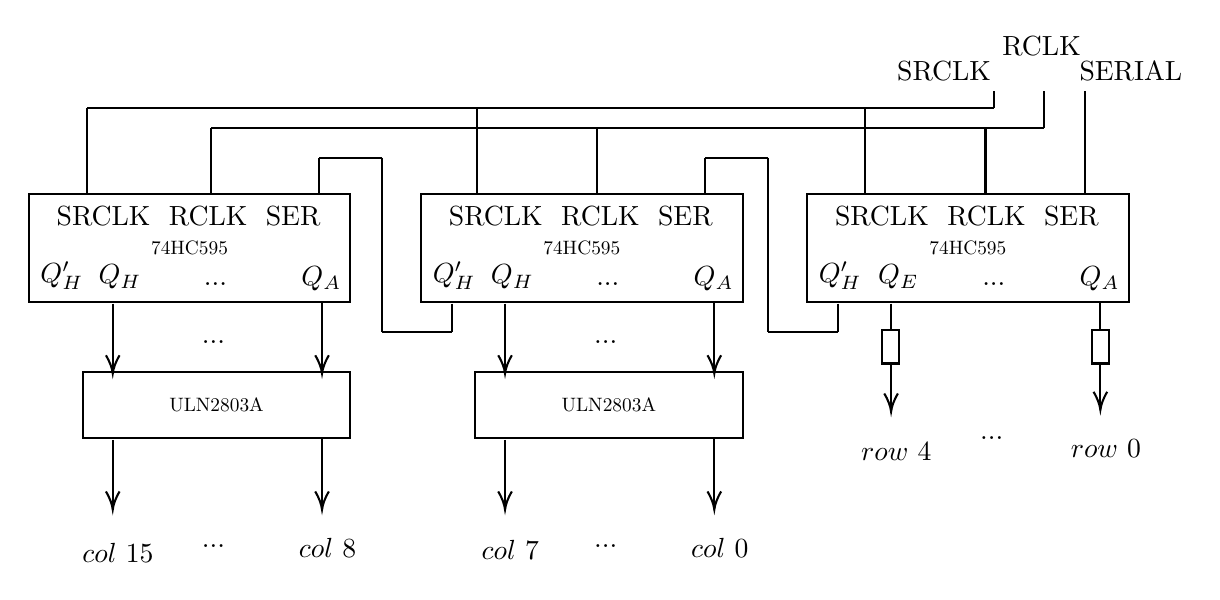
\begin{tikzpicture}[x=0.75pt,y=0.75pt,yscale=-0.8,xscale=1, rotate=90]
		%uncomment if require: \path (0,561); %set diagram left start at 0, and has height of 561
		
		%Shape: Rectangle [id:dp77906780114481] 
		\draw   (199,11) -- (199,166) -- (134,166) -- (134,11) -- cycle ;
		%Straight Lines [id:da4915291358670535] 
		\draw    (200,151) -- (217,151) ;
		
		
		%Straight Lines [id:da49475965092445384] 
		\draw    (217,151) -- (217,185) ;
		
		
		%Straight Lines [id:da8329366668902707] 
		\draw    (199,24.67) -- (233,24.67) ;
		
		
		%Straight Lines [id:da39525289751002846] 
		\draw    (233,24.67) -- (262,24.67) ;
		\draw [shift={(264,24.67)}, rotate = 180] [color={rgb, 255:red, 0; green, 0; blue, 0 }  ][line width=0.75]    (10.93,-3.29) .. controls (6.95,-1.4) and (3.31,-0.3) .. (0,0) .. controls (3.31,0.3) and (6.95,1.4) .. (10.93,3.29)   ;
		
		%Straight Lines [id:da5948093125210301] 
		\draw    (200,125.5) -- (263,125.5) ;
		\draw [shift={(265,125.5)}, rotate = 180] [color={rgb, 255:red, 0; green, 0; blue, 0 }  ][line width=0.75]    (10.93,-3.29) .. controls (6.95,-1.4) and (3.31,-0.3) .. (0,0) .. controls (3.31,0.3) and (6.95,1.4) .. (10.93,3.29)   ;
		
		%Shape: Rectangle [id:dp0608152090495373] 
		\draw   (199,197) -- (199,352) -- (134,352) -- (134,197) -- cycle ;
		%Straight Lines [id:da9054176137392511] 
		\draw    (200,337) -- (217,337) ;
		
		
		%Straight Lines [id:da07810914313886652] 
		\draw    (217,337) -- (217,371) ;
		
		
		%Straight Lines [id:da8248829602234355] 
		\draw    (199,210.67) -- (240,210.67) ;
		\draw [shift={(242,210.67)}, rotate = 180] [color={rgb, 255:red, 0; green, 0; blue, 0 }  ][line width=0.75]    (10.93,-3.29) .. controls (6.95,-1.4) and (3.31,-0.3) .. (0,0) .. controls (3.31,0.3) and (6.95,1.4) .. (10.93,3.29)   ;
		
		%Straight Lines [id:da2215675002986055] 
		\draw    (200,311.5) -- (240,311.5) ;
		\draw [shift={(242,311.5)}, rotate = 180] [color={rgb, 255:red, 0; green, 0; blue, 0 }  ][line width=0.75]    (10.93,-3.29) .. controls (6.95,-1.4) and (3.31,-0.3) .. (0,0) .. controls (3.31,0.3) and (6.95,1.4) .. (10.93,3.29)   ;
		
		%Shape: Rectangle [id:dp42192978019148053] 
		\draw   (199,386) -- (199,541) -- (134,541) -- (134,386) -- cycle ;
		%Straight Lines [id:da15739771667206748] 
		\draw    (199,399.67) -- (240,399.67) ;
		\draw [shift={(242,399.67)}, rotate = 180] [color={rgb, 255:red, 0; green, 0; blue, 0 }  ][line width=0.75]    (10.93,-3.29) .. controls (6.95,-1.4) and (3.31,-0.3) .. (0,0) .. controls (3.31,0.3) and (6.95,1.4) .. (10.93,3.29)   ;
		
		%Straight Lines [id:da0647979687710658] 
		\draw    (200,500.5) -- (240,500.5) ;
		\draw [shift={(242,500.5)}, rotate = 180] [color={rgb, 255:red, 0; green, 0; blue, 0 }  ][line width=0.75]    (10.93,-3.29) .. controls (6.95,-1.4) and (3.31,-0.3) .. (0,0) .. controls (3.31,0.3) and (6.95,1.4) .. (10.93,3.29)   ;
		
		%Straight Lines [id:da8676553847091906] 
		\draw    (112,185) -- (217,185) ;
		
		
		%Straight Lines [id:da3415766479334226] 
		\draw    (112,185) -- (112,215) ;
		
		
		%Straight Lines [id:da6142122840146302] 
		\draw    (112,215) -- (134,215) ;
		
		
		%Straight Lines [id:da9652390765642762] 
		\draw    (112,371) -- (217,371) ;
		
		
		%Straight Lines [id:da9292046463897523] 
		\draw    (112,371) -- (112,401) ;
		
		
		%Straight Lines [id:da9168684409494134] 
		\draw    (112,401) -- (134,401) ;
		
		
		%Straight Lines [id:da6046337623247116] 
		\draw    (134,32) -- (72,32) ;
		
		
		%Straight Lines [id:da8864424911216267] 
		\draw    (72,52) -- (94,52) ;
		
		
		%Straight Lines [id:da4882456086801612] 
		\draw    (94,52) -- (94,453) ;
		
		
		%Straight Lines [id:da73120440781388] 
		\draw    (134,80) -- (94,80) ;
		
		
		%Straight Lines [id:da22234880884598196] 
		\draw    (134,267) -- (94,267) ;
		
		
		%Straight Lines [id:da7881327020454503] 
		\draw    (134,453) -- (94,453) ;
		
		
		%Straight Lines [id:da8117366129977888] 
		\draw    (72,76) -- (82,76) ;
		
		
		%Straight Lines [id:da47614413495920704] 
		\draw    (82,76) -- (82,513) ;
		
		
		%Straight Lines [id:da42042074982877997] 
		\draw    (134,138) -- (82,138) ;
		
		
		%Straight Lines [id:da22056366978165554] 
		\draw    (134,325) -- (82,325) ;
		
		
		%Straight Lines [id:da8409220597549094] 
		\draw    (134,513) -- (82,513) ;
		
		
		%Shape: Rectangle [id:dp044387012327000486] 
		\draw   (281,197) -- (281,326) -- (241,326) -- (241,197) -- cycle ;
		%Straight Lines [id:da44580338729319413] 
		\draw    (281,210.67) -- (322,210.67) ;
		\draw [shift={(324,210.67)}, rotate = 180] [color={rgb, 255:red, 0; green, 0; blue, 0 }  ][line width=0.75]    (10.93,-3.29) .. controls (6.95,-1.4) and (3.31,-0.3) .. (0,0) .. controls (3.31,0.3) and (6.95,1.4) .. (10.93,3.29)   ;
		
		%Straight Lines [id:da6971901407200194] 
		\draw    (282,311.5) -- (322,311.5) ;
		\draw [shift={(324,311.5)}, rotate = 180] [color={rgb, 255:red, 0; green, 0; blue, 0 }  ][line width=0.75]    (10.93,-3.29) .. controls (6.95,-1.4) and (3.31,-0.3) .. (0,0) .. controls (3.31,0.3) and (6.95,1.4) .. (10.93,3.29)   ;
		
		%Shape: Rectangle [id:dp5761512718357171] 
		\draw   (281,386) -- (281,515) -- (241,515) -- (241,386) -- cycle ;
		%Straight Lines [id:da9992647385686131] 
		\draw    (281,399.67) -- (322,399.67) ;
		\draw [shift={(324,399.67)}, rotate = 180] [color={rgb, 255:red, 0; green, 0; blue, 0 }  ][line width=0.75]    (10.93,-3.29) .. controls (6.95,-1.4) and (3.31,-0.3) .. (0,0) .. controls (3.31,0.3) and (6.95,1.4) .. (10.93,3.29)   ;
		
		%Straight Lines [id:da6824737498679518] 
		\draw    (282,500.5) -- (322,500.5) ;
		\draw [shift={(324,500.5)}, rotate = 180] [color={rgb, 255:red, 0; green, 0; blue, 0 }  ][line width=0.75]    (10.93,-3.29) .. controls (6.95,-1.4) and (3.31,-0.3) .. (0,0) .. controls (3.31,0.3) and (6.95,1.4) .. (10.93,3.29)   ;
		
		%Shape: Rectangle [id:dp5642253019817809] 
		\draw  [fill={rgb, 255:red, 255; green, 255; blue, 255 }  ,fill opacity=1 ] (216,20.67) -- (236,20.67) -- (236,28.67) -- (216,28.67) -- cycle ;
		%Shape: Rectangle [id:dp13422121953986577] 
		\draw  [fill={rgb, 255:red, 255; green, 255; blue, 255 }  ,fill opacity=1 ] (216,121.67) -- (236,121.67) -- (236,129.67) -- (216,129.67) -- cycle ;
		
		
		% Text Node
		\draw (147,89) node [rotate=0] [align=left] {SRCLK \ RCLK \ SER};
		% Text Node
		\draw (185,25) node   {$Q_{A}$};
		% Text Node
		\draw (184,122) node   {$Q_{E}$};
		% Text Node
		\draw (183,150) node   {$Q_{H} '$};
		% Text Node
		\draw (188,76) node [rotate=0] [align=left] {...};
		% Text Node
		\draw (60,100) node  [align=left, rotate=0] {SRCLK};
		% Text Node
		\draw (45,53) node  [align=left, rotate=0] {RCLK};
		% Text Node
		\draw (287,22) node   {$row\ 0$};
		% Text Node
		\draw (289,123) node   {$row\ 4$};
		% Text Node
		\draw (281,77) node [rotate=0] [align=left] {...};
		% Text Node
		\draw (147,275) node [rotate=0] [align=left] {SRCLK \ RCLK \ SER};
		% Text Node
		\draw (185,211) node   {$Q_{A}$};
		% Text Node
		\draw (184,308) node   {$Q_{H}$};
		% Text Node
		\draw (183,336) node   {$Q_{H} '$};
		% Text Node
		\draw (188,262) node [rotate=0] [align=left] {...};
		% Text Node
		\draw (347,208) node   {$col\ 0$};
		% Text Node
		\draw (348,309) node   {$col\ 7$};
		% Text Node
		\draw (223,263) node [rotate=0] [align=left] {...};
		% Text Node
		\draw (147,464) node [rotate=0] [align=left] {SRCLK \ RCLK \ SER};
		% Text Node
		\draw (185,400) node   {$Q_{A}$};
		% Text Node
		\draw (184,497) node   {$Q_{H}$};
		% Text Node
		\draw (183,525) node   {$Q_{H} '$};
		% Text Node
		\draw (188,451) node [rotate=0] [align=left] {...};
		% Text Node
		\draw (347,397) node   {$col\ 8$};
		% Text Node
		\draw (350,498) node   {$col\ 15$};
		% Text Node
		\draw (223,452) node [rotate=0] [align=left] {...};
		% Text Node
		\draw (60,10) node  [align=left, rotate=00] {SERIAL};
		% Text Node
		\draw (166.5,88.5) node [scale=0.7,rotate=0] [align=left] {74HC595};
		% Text Node
		\draw (166.5,274.5) node [scale=0.7,rotate=0] [align=left] {74HC595};
		% Text Node
		\draw (166.5,463.5) node [scale=0.7,rotate=0] [align=left] {74HC595};
		% Text Node
		\draw (261,261.5) node [scale=0.7,rotate=0] [align=left] {ULN2803A};
		% Text Node
		\draw (261,450.5) node [scale=0.7,rotate=0] [align=left] {ULN2803A};
		% Text Node
		\draw (346,263) node [rotate=0] [align=left] {...};
		% Text Node
		\draw (346,452) node [rotate=0] [align=left] {...};
		
		
		\end{tikzpicture}
		\caption{ULN2803A Option to drive the columns \cite{ledsULN}}	
		\label{sfig:sr2803}
	\end{subfigure}
	\caption{Circuit Designs for driving the \acap{led}}
	\label{fig:srLedOptions}
\end{figure}\\
As can be seen in Figure \ref{fig:srLedOptions}, the chosen \ac{sipo} Shift Register is the 74HC595 \cite{595}. This type of shift register will hold its value as it has an output buffer which in turn reduces flickering of the \acap{led} as they stay on for as long as possible \cite{srOpenMusic}. \\
Resistors will be connected to each of the driver pins, in this case, the rows. These resistors will restrict the current that can flow through the \ac{led} connected to the respective row. 
\begin{equation}
	\label{eqn:RowRes}
	\begin{split}
	R &= \frac{V_{CC} - V_{f(LED)}}{I_{max (LED)}}\\
	&= \frac{3.3 - 2.0}{30m}\\
	&= 43.33\Omega \approx 47\Omega
	\end{split}
\end{equation}
The resistance calculations for the resistor in each row are shown in Equation \ref{eqn:RowRes}. This uses the chosen LTST-C150KFKT \ac{led}'s values for maximum forward current and forward voltage \cite{led}. The value of 43.33$\Omega$ represents the minimum resistance value for the resistor to have before the maximum forward current of 30mA is surpassed. To allow for some tolerance, as well as selecting a standard value resistor, the value of 47$\Omega$ is selected.\\
In the current configuration, each column pin will experience a maximum of $5$ rows $ * 30$mA $=150$mA. For this reason, the ULN2803A variant is the only one capable of draining the current of the rows effectively. Even though this system is being cycled through at high speed, it is safer to consider the continuous current ratings as opposed to the maximal pulsing ratings.\\
A design which could prove more efficient than that chosen would be to invert how the \acap{led} are places and use the rows to drain the current and columns to drive the state. If this technique was used there would be one less ULN2803A \ac{ic}, and there would be fewer iterations in software as now up to sixteen \acap{led} can be lit up simultaneously as opposed to the five from the current technique. Considering the maximal current of the ULN2803A, it can be seen that this technique would still fall in the safe boundary: $16$ cols $* 30$mA $=480$mA.
\section{Tempo and Volume Control}
Perhaps the simplest methods of interaction for the end user are the tempo and volume control knobs. As the names imply, there will be two methods for the user to change the tempo (\ac{bpm}), and volume of the sounds scheduled and produced by the system.
\subsection{Methods to Measure Rotation}
Two methods to measure how much the end user has rotated a knob are considered: a potentiometer, and an incremental rotary encoder.\\ 
\textbf{Rotary Encoders} come in many variations, however, in this situation only one type, the incremental rotary encoder will be considered. This is the simplest type of rotary encoder as it simply has voltage supply lines with two outputs that have a $90^\circ$ phase offset from one another. 
\begin{figure}[h!]
	\centering
	\begin{subfigure}[b]{0.48\textwidth}
		\centering
		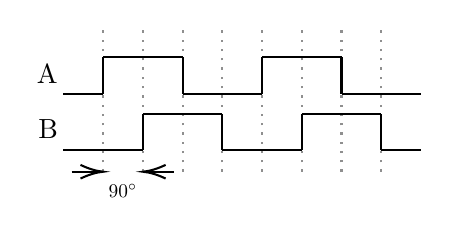
\begin{tikzpicture}[x=0.75pt,y=0.75pt,yscale=-1,xscale=1]
		%uncomment if require: \path (0,171); %set diagram left start at 0, and has height of 171
		
		%Straight Lines [id:da7885955371927524] 
		\draw [color={rgb, 255:red, 143; green, 143; blue, 143 }  ,draw opacity=1 ] [dash pattern={on 0.84pt off 2.51pt}]  (46.14,129) -- (46.14,60.1) ;
		
		
		%Straight Lines [id:da7188942249290038] 
		\draw [color={rgb, 255:red, 143; green, 143; blue, 143 }  ,draw opacity=1 ] [dash pattern={on 0.84pt off 2.51pt}]  (65.28,129) -- (65.28,60.1) ;
		
		
		%Straight Lines [id:da9280048778513557] 
		\draw [color={rgb, 255:red, 143; green, 143; blue, 143 }  ,draw opacity=1 ] [dash pattern={on 0.84pt off 2.51pt}]  (84.42,129) -- (84.42,60.1) ;
		
		
		%Straight Lines [id:da7787877106041785] 
		\draw [color={rgb, 255:red, 143; green, 143; blue, 143 }  ,draw opacity=1 ] [dash pattern={on 0.84pt off 2.51pt}]  (103.56,129) -- (103.56,60.1) ;
		
		
		%Straight Lines [id:da6714125221545921] 
		\draw [color={rgb, 255:red, 143; green, 143; blue, 143 }  ,draw opacity=1 ] [dash pattern={on 0.84pt off 2.51pt}]  (122.69,129) -- (122.69,60.1) ;
		
		
		%Straight Lines [id:da14200907321221812] 
		\draw [color={rgb, 255:red, 143; green, 143; blue, 143 }  ,draw opacity=1 ] [dash pattern={on 0.84pt off 2.51pt}]  (141.83,129) -- (141.83,60.1) ;
		
		
		%Straight Lines [id:da5880284570305154] 
		\draw [color={rgb, 255:red, 143; green, 143; blue, 143 }  ,draw opacity=1 ] [dash pattern={on 0.84pt off 2.51pt}]  (160.97,129) -- (160.97,60.1) ;
		
		
		%Straight Lines [id:da8701787686391249] 
		\draw [color={rgb, 255:red, 143; green, 143; blue, 143 }  ,draw opacity=1 ] [dash pattern={on 0.84pt off 2.51pt}]  (180.11,129) -- (180.11,60.1) ;
		
		
		%Straight Lines [id:da7761468539721306] 
		\draw    (27,91.41) -- (46.14,91.41) ;
		
		
		%Straight Lines [id:da725890584751314] 
		\draw    (46.14,73.63) -- (65.28,73.63) ;
		
		
		%Straight Lines [id:da5544515896885982] 
		\draw    (46.14,91.41) -- (46.14,73.63) ;
		
		
		%Straight Lines [id:da3996834516495007] 
		\draw    (84.42,91.41) -- (84.42,73.63) ;
		
		
		%Straight Lines [id:da9006942093663342] 
		\draw    (65.28,73.63) -- (84.42,73.63) ;
		
		
		%Straight Lines [id:da5756500064774586] 
		\draw    (84.42,91.41) -- (103.56,91.41) ;
		
		
		%Straight Lines [id:da02499464530443607] 
		\draw    (103.56,91.41) -- (122.69,91.41) ;
		
		
		%Straight Lines [id:da4610215518491947] 
		\draw    (122.69,73.63) -- (141.83,73.63) ;
		
		
		%Straight Lines [id:da42994349821241573] 
		\draw    (122.69,91.41) -- (122.69,73.63) ;
		
		
		%Straight Lines [id:da23398470501090363] 
		\draw    (160.97,91.41) -- (160.97,73.63) ;
		
		
		%Straight Lines [id:da33475843964666074] 
		\draw    (141.83,73.63) -- (160.97,73.63) ;
		
		
		%Straight Lines [id:da35572312665104655] 
		\draw    (160.97,91.41) -- (180.11,91.41) ;
		
		
		%Straight Lines [id:da09520385048937552] 
		\draw    (180.11,91.41) -- (199.25,91.41) ;
		
		
		%Straight Lines [id:da8604436141325764] 
		\draw    (46.14,118.75) -- (65.28,118.75) ;
		
		
		%Straight Lines [id:da03580503923224598] 
		\draw    (65.28,100.98) -- (84.42,100.98) ;
		
		
		%Straight Lines [id:da33247672804926287] 
		\draw    (65.28,118.75) -- (65.28,100.98) ;
		
		
		%Straight Lines [id:da049939777709399724] 
		\draw    (103.56,118.75) -- (103.56,100.98) ;
		
		
		%Straight Lines [id:da23729782058634674] 
		\draw    (84.42,100.98) -- (103.56,100.98) ;
		
		
		%Straight Lines [id:da5012714490951418] 
		\draw    (103.56,118.75) -- (122.69,118.75) ;
		
		
		%Straight Lines [id:da7647630568444796] 
		\draw    (122.69,118.75) -- (141.83,118.75) ;
		
		
		%Straight Lines [id:da7286190954368377] 
		\draw    (141.83,100.98) -- (160.97,100.98) ;
		
		
		%Straight Lines [id:da7524598510359293] 
		\draw    (141.83,118.75) -- (141.83,100.98) ;
		
		
		%Straight Lines [id:da04268234260045212] 
		\draw    (180.11,118.75) -- (180.11,100.98) ;
		
		
		%Straight Lines [id:da2396980482457376] 
		\draw    (160.97,100.98) -- (180.11,100.98) ;
		
		
		%Straight Lines [id:da7930386051110299] 
		\draw    (180.11,118.75) -- (199.25,118.75) ;
		
		
		%Straight Lines [id:da20475027941663027] 
		\draw    (27,118.75) -- (46.14,118.75) ;
		
		
		%Straight Lines [id:da5519376712939885] 
		\draw    (30.94,129) -- (44.14,129) ;
		\draw [shift={(46.14,129)}, rotate = 180] [color={rgb, 255:red, 0; green, 0; blue, 0 }  ][line width=0.75]    (10.93,-3.29) .. controls (6.95,-1.4) and (3.31,-0.3) .. (0,0) .. controls (3.31,0.3) and (6.95,1.4) .. (10.93,3.29)   ;
		
		%Straight Lines [id:da47487088745634054] 
		\draw    (67.28,129) -- (80.48,129) ;
		
		\draw [shift={(65.28,129)}, rotate = 0] [color={rgb, 255:red, 0; green, 0; blue, 0 }  ][line width=0.75]    (10.93,-3.29) .. controls (6.95,-1.4) and (3.31,-0.3) .. (0,0) .. controls (3.31,0.3) and (6.95,1.4) .. (10.93,3.29)   ;
		
		% Text Node
		\draw (55.6,138.4) node [scale=0.7]  {$90^\circ $};
		% Text Node
		\draw (19.2,82) node  [align=left] {A};
		% Text Node
		\draw (19.6,108.6) node  [align=left] {B};
		
		
		\end{tikzpicture}
		\caption{Clockwise Rotation Output}	
	\end{subfigure}
	\hfill
	\begin{subfigure}[b]{0.48\textwidth}
		\centering
		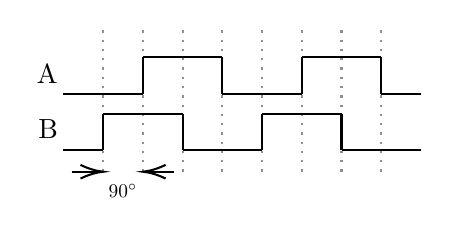
\begin{tikzpicture}[x=0.75pt,y=0.75pt,yscale=-1,xscale=1]
		%uncomment if require: \path (0,159); %set diagram left start at 0, and has height of 159
		
		%Straight Lines [id:da900134298796494] 
		\draw [color={rgb, 255:red, 143; green, 143; blue, 143 }  ,draw opacity=1 ] [dash pattern={on 0.84pt off 2.51pt}]  (46.14,129) -- (46.14,60.1) ;
		
		
		%Straight Lines [id:da2788352326327088] 
		\draw [color={rgb, 255:red, 143; green, 143; blue, 143 }  ,draw opacity=1 ] [dash pattern={on 0.84pt off 2.51pt}]  (65.28,129) -- (65.28,60.1) ;
		
		
		%Straight Lines [id:da9580427595769845] 
		\draw [color={rgb, 255:red, 143; green, 143; blue, 143 }  ,draw opacity=1 ] [dash pattern={on 0.84pt off 2.51pt}]  (84.42,129) -- (84.42,60.1) ;
		
		
		%Straight Lines [id:da41756282410421] 
		\draw [color={rgb, 255:red, 143; green, 143; blue, 143 }  ,draw opacity=1 ] [dash pattern={on 0.84pt off 2.51pt}]  (103.56,129) -- (103.56,60.1) ;
		
		
		%Straight Lines [id:da8293313141483531] 
		\draw [color={rgb, 255:red, 143; green, 143; blue, 143 }  ,draw opacity=1 ] [dash pattern={on 0.84pt off 2.51pt}]  (122.69,129) -- (122.69,60.1) ;
		
		
		%Straight Lines [id:da9446965826165783] 
		\draw [color={rgb, 255:red, 143; green, 143; blue, 143 }  ,draw opacity=1 ] [dash pattern={on 0.84pt off 2.51pt}]  (141.83,129) -- (141.83,60.1) ;
		
		
		%Straight Lines [id:da38818434205440466] 
		\draw [color={rgb, 255:red, 143; green, 143; blue, 143 }  ,draw opacity=1 ] [dash pattern={on 0.84pt off 2.51pt}]  (160.97,129) -- (160.97,60.1) ;
		
		
		%Straight Lines [id:da6266416548104501] 
		\draw [color={rgb, 255:red, 143; green, 143; blue, 143 }  ,draw opacity=1 ] [dash pattern={on 0.84pt off 2.51pt}]  (180.11,129) -- (180.11,60.1) ;
		
		
		%Straight Lines [id:da26045043950308355] 
		\draw    (27,91.41) -- (46.14,91.41) ;
		
		
		%Straight Lines [id:da018423870418572852] 
		\draw    (46.14,91.41) -- (65.28,91.41) ;
		
		
		%Straight Lines [id:da19508629660870636] 
		\draw    (65.28,91.41) -- (65.28,73.63) ;
		
		
		%Straight Lines [id:da4712839489226013] 
		\draw    (103.56,91.41) -- (103.56,73.63) ;
		
		
		%Straight Lines [id:da16398064823756897] 
		\draw    (65.28,73.63) -- (84.42,73.63) ;
		
		
		%Straight Lines [id:da10438159661926538] 
		\draw    (84.42,73.63) -- (103.56,73.63) ;
		
		
		%Straight Lines [id:da837802874492384] 
		\draw    (103.56,91.41) -- (122.69,91.41) ;
		
		
		%Straight Lines [id:da6899148804893396] 
		\draw    (122.69,91.41) -- (141.83,91.41) ;
		
		
		%Straight Lines [id:da013328718745104773] 
		\draw    (141.83,91.41) -- (141.83,73.63) ;
		
		
		%Straight Lines [id:da7755401681612648] 
		\draw    (180.11,91.41) -- (180.11,73.63) ;
		
		
		%Straight Lines [id:da7023537709271184] 
		\draw    (141.83,73.63) -- (160.97,73.63) ;
		
		
		%Straight Lines [id:da9147264507755728] 
		\draw    (160.97,73.63) -- (180.11,73.63) ;
		
		
		%Straight Lines [id:da3383934568959077] 
		\draw    (180.11,91.41) -- (199.25,91.41) ;
		
		
		%Straight Lines [id:da06685288883167684] 
		\draw    (46.14,100.98) -- (65.28,100.98) ;
		
		
		%Straight Lines [id:da18404953583430683] 
		\draw    (65.28,100.98) -- (84.42,100.98) ;
		
		
		%Straight Lines [id:da6107329886153519] 
		\draw    (46.14,118.75) -- (46.14,100.98) ;
		
		
		%Straight Lines [id:da5076229808454147] 
		\draw    (84.42,118.75) -- (84.42,100.98) ;
		
		
		%Straight Lines [id:da9205201817900404] 
		\draw    (84.42,118.75) -- (103.56,118.75) ;
		
		
		%Straight Lines [id:da39159250930967815] 
		\draw    (103.56,118.75) -- (122.69,118.75) ;
		
		
		%Straight Lines [id:da9824954812007205] 
		\draw    (122.69,100.98) -- (141.83,100.98) ;
		
		
		%Straight Lines [id:da8750438092850736] 
		\draw    (141.83,100.98) -- (160.97,100.98) ;
		
		
		%Straight Lines [id:da10006344416572621] 
		\draw    (122.69,118.75) -- (122.69,100.98) ;
		
		
		%Straight Lines [id:da5732381842696901] 
		\draw    (160.97,118.75) -- (160.97,100.98) ;
		
		
		%Straight Lines [id:da5449186565200632] 
		\draw    (160.97,118.75) -- (180.11,118.75) ;
		
		
		%Straight Lines [id:da9414927851281742] 
		\draw    (180.11,118.75) -- (199.25,118.75) ;
		
		
		%Straight Lines [id:da960258312365353] 
		\draw    (27,118.75) -- (46.14,118.75) ;
		
		
		%Straight Lines [id:da07390759227633392] 
		\draw    (30.94,129) -- (44.14,129) ;
		\draw [shift={(46.14,129)}, rotate = 180] [color={rgb, 255:red, 0; green, 0; blue, 0 }  ][line width=0.75]    (10.93,-3.29) .. controls (6.95,-1.4) and (3.31,-0.3) .. (0,0) .. controls (3.31,0.3) and (6.95,1.4) .. (10.93,3.29)   ;
		
		%Straight Lines [id:da9888166560035792] 
		\draw    (67.28,129) -- (80.48,129) ;
		
		\draw [shift={(65.28,129)}, rotate = 0] [color={rgb, 255:red, 0; green, 0; blue, 0 }  ][line width=0.75]    (10.93,-3.29) .. controls (6.95,-1.4) and (3.31,-0.3) .. (0,0) .. controls (3.31,0.3) and (6.95,1.4) .. (10.93,3.29)   ;
		
		% Text Node
		\draw (55.6,138.4) node [scale=0.7]  {$90^\circ $};
		% Text Node
		\draw (19.2,82) node  [align=left] {A};
		% Text Node
		\draw (19.6,108.6) node  [align=left] {B};
		
		
		\end{tikzpicture}
		\caption{Counter Clockwise Rotation Output}
	\end{subfigure}
	\caption{Rotary Encoder Outputs \cite{rotEnc}}
	\label{fig:rotenc}
\end{figure}
Figure \ref{fig:rotenc} shows the two output pins from a rotary encoder \cite{rotEnc}. From this it can be seen that if signal B lags behind signal A the rotary encoder is turned clockwise and visa versa. Rotary Encoders allow for unlimited revolutions in either direction as they simply show which direction they are being turned, they, however, require two pins to read the signal as well as timers on the \ac{uc} \cite{rotEnc}.\\
\textbf{Potentiometers} are a far simpler and more rudimentary technique. A potentiometer can be used as a voltage divider circuit by placing it between ground (0V) potential and the supply voltage ($V_{cc}$). The wiper pin can then be the voltage divided using Equation \ref{eqn:voltDiv}. In this equation, $R_{gnd}$ refers to the resistance from the wiper to ground and $R_{vcc}$ refers to the resistance from the wiper to $V_{cc}$.
\begin{equation} \label{eqn:voltDiv}
	V_{div} = V_{cc} * \frac{R_{gnd}}{R_{vcc} + R_{gnd}}
\end{equation}\\
To interpret the voltage value $V_{div}$ an \ac{adc} must be used on the \ac{uc} \cite{f411}. The \ac{adc} will measure the voltage digitally as the number of steps between zero and the size limit it is set to, for example, a 12-bit buffer will allow a value between 0 and $2^{12}-1 = 4095$. If $V_{div}$ was $0.5 V_{cc}$ then the value from the \ac{adc} will be $(0.5 * 2^{12})-1 = 2047$. The potentiometer method has the benefit of only having one wire going to the \ac{adc} on the \ac{uc}. On the other hand, a potentiometer cannot turn more than a set angle, usually $270^\circ$ or more.
\newpage
\subsection{Chosen Method}
Due to the simplicity of the potentiometer circuit, it can be used for both the volume and tempo control. The limited amount which the user can turn the potentiometers allows an association between a value and a position. For example, if the user wants the volume at 50\% then they can set the potentiometer for volume half way and know that that position will always yield the same volume value. Similarly, for the tempo, it could prove useful to have a set range limited in software. The chosen potentiometers have a value of 10k$\Omega$ and are linear over $270^\circ$ \cite{pot}. \\
An offset was added to the tempo potentiometer by soldering a resistor between the potentiometer and $V_{cc}$. This resistor reduced the maximum tempo and its value was determined with Equation \ref{eqn:potOffs}. $S_{max}$ is the fraction to which the tempo must be limited compared to its prior maximum.
\begin{equation} \label{eqn:potOffs}
\begin{aligned}
S_{max} &= \frac{R_{gnd}}{R_{vcc} + R_{gnd} + R_{offs}} &\\
R_{offs} &= - R_{vcc} - \Big( 1 - \frac{1}{S_{max}} \Big) R_{gnd} &\\
&= \Big(\frac{1}{S_{max}} - 1 \Big) R_{pot} &\text{when}\ R_{vcc} = 0, \ R_{gnd} = R_{pot}
\end{aligned}
\end{equation}\\
The desired fraction, $S_{max}$, is chosen to be 87\% as this reduces the maximum \ac{bpm} low enough to be useful. This results in the $R_{offs}$ value being 1494$\Omega$, this is then rounded to 1.5k$\Omega$. This value limits the \ac{bpm} to approximately 485.
\section{LCD}
The tempo and volume values that are controlled by the \ac{uc} and potentiometers, as discussed prior, are displayed to the user using a \ac{lcd}. This \ac{lcd} must update frequently enough for the user to constantly know the displayed values in real time.
\subsection{Driving a Parallel LCD}
The \ac{lcd} that is selected is the PC1601A \cite{lcd} due to its availability at the University and its use in prior projects, with readily available driver source code. This \ac{lcd} is sixteen characters wide and one row high \cite{lcd}. It is driven by a 6800 4/8-bit parallel interface in 4-bit (nibble) mode, this way only four pins are needed to control the data flow to and from the \ac{lcd} \cite{lcd}. Running the display in nibble mode means that four extra pins are being traded in for double the time to read or write one byte of data to or from the display. Other than the data pins, the \ac{lcd} must also be controlled with three control lines: Enable (E), Read not Write (RNW), and Register Select (RS) \cite{lcd}. All seven pins will be connected to the \ac{uc}'s \ac{gpio} pins. Even though the \ac{lcd} is powered by a 5V supply it can be controlled by 3.3V logic coming from the \ac{uc} as $V_{IH} \geq 2.2\text{V}$ \cite{lcd}.\\
To control the contrast of the \ac{lcd} there is a pin, labeled $V_O$, which must act as a voltage divider circuit (See Equation \ref{eqn:voltDiv}). As per the datasheet \cite{lcd}, a trimmer potentiometer of 20k$\Omega$ is used to divide between 5V and Ground, it is adjusted manually until the desired contrast is reached.
\section{Serial Communication with a PC}
The serial communication connection to a PC is an optional feature being used as a debugging tool during the development of the complete system.
\subsection{Reason for implementation}
This interface was added as a debugging tool during the development phase, however, it was also included as an option to upgrade the system at a later stage, time permitting. This upgrade would come in the form of \ac{midi} support over \ac{usb}. \ac{midi} is based on a serial communication protocol \cite{midiUart} which can be substituted with the \ac{uart} protocol. This additional feature was not added due to time restrictions. 
\subsection{Circuit Design}
The base circuit design, as well as the breakout board used, comes from the Design E314 Module.
\begin{figure}[h!]
	\centering
	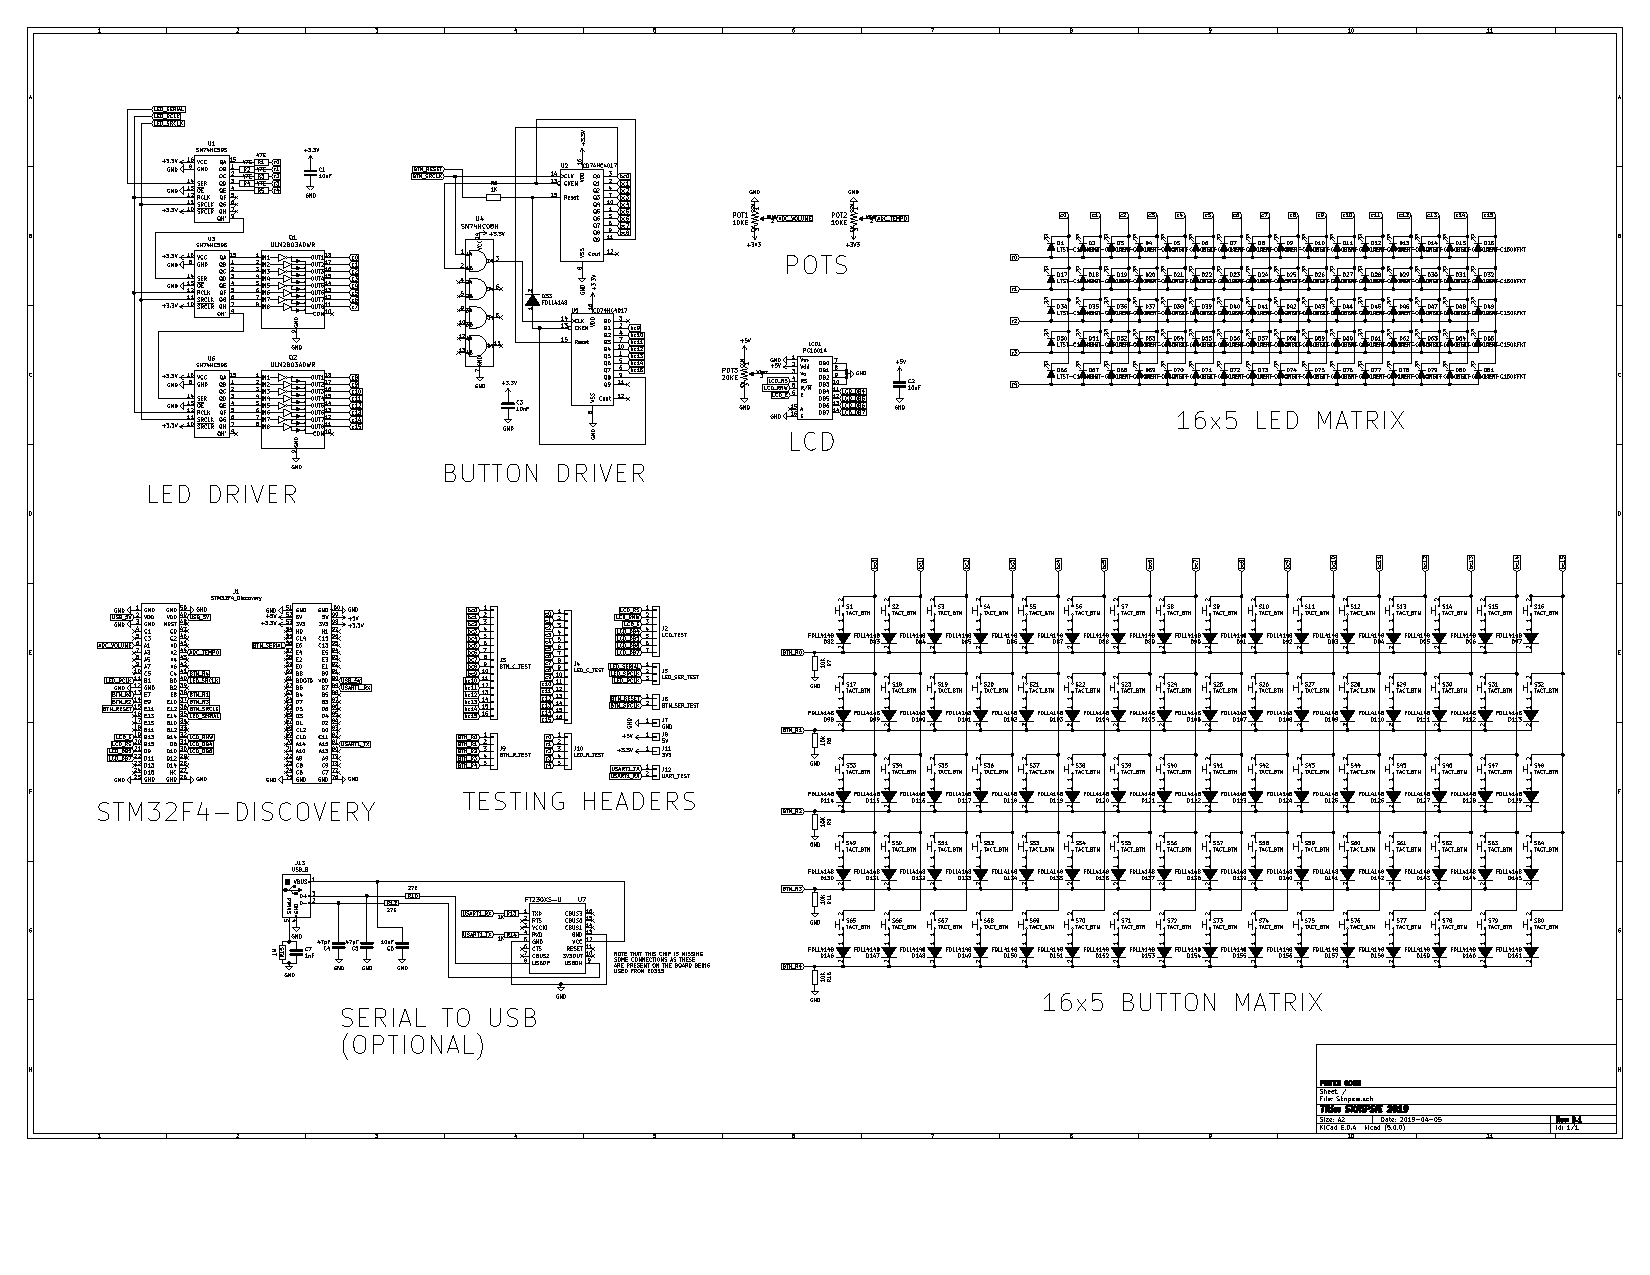
\includegraphics[width = 0.7\textwidth, origin=c, trim={1.75in 1.8in 6in 5.72in}, clip]{../Skripsie/Layout_05042019.pdf}
	\caption{Circuit Diagram for Serial Communication \cite{ft230x}}
	\label{fig:ft230xsCompl}
\end{figure}
Shown in Figure \ref{fig:ft230xsCompl} is the FT230-XS \ac{uart} to \ac{usb} \ac{ic} \cite{ft230x} is used for this feature connected to a \ac{usb} type-A connector. All necessary resistors and capacitors are included as per the typical configuration to be powered by \ac{usb} bus power \cite{ft230x}. Data and power lines from the \ac{usb} connector are all connected through capacitors to ground, 47pF and 10nF respectively, to suppress any \ac{ac} noise on these lines. Resistors placed on the \ac{usb} data lines are 27$\Omega$ to reduce the maximum current. 1k$\Omega$ resistors are placed on the \ac{uart} TX and RX connections to reduce parasitic currents between the \ac{uc} and FT230-XS \ac{ic}.
\begin{figure}[h!]
	\centering
	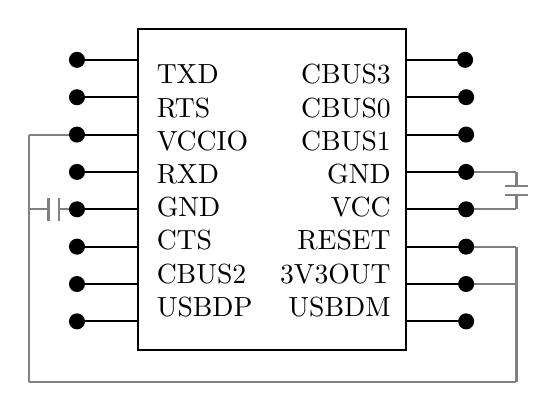
\begin{tikzpicture}[x=0.75pt,y=0.75pt,yscale=-1,xscale=1]
	%uncomment if require: \path (0,412); %set diagram left start at 0, and has height of 412
	
	%Straight Lines [id:da9246066076828634] 
	\draw [color={rgb, 255:red, 128; green, 128; blue, 128 }  ,draw opacity=1 ]   (355.25,139) -- (331,139) ;
	
	
	%Straight Lines [id:da7662467232416275] 
	\draw [color={rgb, 255:red, 128; green, 128; blue, 128 }  ,draw opacity=1 ]   (331,193) -- (355.25,193) ;
	
	
	%Straight Lines [id:da9091545634597022] 
	\draw [color={rgb, 255:red, 128; green, 128; blue, 128 }  ,draw opacity=1 ]   (355.25,175) -- (331,175) ;
	
	
	%Straight Lines [id:da3519821670961991] 
	\draw [color={rgb, 255:red, 128; green, 128; blue, 128 }  ,draw opacity=1 ]   (355.25,157) -- (331,157) ;
	
	
	%Straight Lines [id:da7026317077799362] 
	\draw [color={rgb, 255:red, 128; green, 128; blue, 128 }  ,draw opacity=1 ]   (144,157) -- (134.8,157) ;
	\draw [shift={(134.8,157)}, rotate = 360] [color={rgb, 255:red, 128; green, 128; blue, 128 }  ,draw opacity=1 ][line width=0.75]    (0,5.59) -- (0,-5.59)   ;
	
	%Straight Lines [id:da48266600054773834] 
	\draw [color={rgb, 255:red, 128; green, 128; blue, 128 }  ,draw opacity=1 ]   (144,121) -- (120.25,121) ;
	
	
	%Shape: Rectangle [id:dp4825549281189261] 
	\draw   (173,70) -- (302,70) -- (302,225) -- (173,225) -- cycle ;
	
	%Straight Lines [id:da08516907367262805] 
	\draw    (143.5,85) -- (172.5,85) ;
	
	\draw [shift={(143.5,85)}, rotate = 0] [color={rgb, 255:red, 0; green, 0; blue, 0 }  ][fill={rgb, 255:red, 0; green, 0; blue, 0 }  ][line width=0.75]      (0, 0) circle [x radius= 3.35, y radius= 3.35]   ;
	%Straight Lines [id:da37716082123749906] 
	\draw    (143.5,103) -- (172.5,103) ;
	
	\draw [shift={(143.5,103)}, rotate = 0] [color={rgb, 255:red, 0; green, 0; blue, 0 }  ][fill={rgb, 255:red, 0; green, 0; blue, 0 }  ][line width=0.75]      (0, 0) circle [x radius= 3.35, y radius= 3.35]   ;
	%Straight Lines [id:da5202986803813208] 
	\draw    (143.5,121) -- (172.5,121) ;
	
	\draw [shift={(143.5,121)}, rotate = 0] [color={rgb, 255:red, 0; green, 0; blue, 0 }  ][fill={rgb, 255:red, 0; green, 0; blue, 0 }  ][line width=0.75]      (0, 0) circle [x radius= 3.35, y radius= 3.35]   ;
	%Straight Lines [id:da04712389509347603] 
	\draw    (143.5,139) -- (172.5,139) ;
	
	\draw [shift={(143.5,139)}, rotate = 0] [color={rgb, 255:red, 0; green, 0; blue, 0 }  ][fill={rgb, 255:red, 0; green, 0; blue, 0 }  ][line width=0.75]      (0, 0) circle [x radius= 3.35, y radius= 3.35]   ;
	%Straight Lines [id:da26840776853069626] 
	\draw    (143.5,157) -- (172.5,157) ;
	
	\draw [shift={(143.5,157)}, rotate = 0] [color={rgb, 255:red, 0; green, 0; blue, 0 }  ][fill={rgb, 255:red, 0; green, 0; blue, 0 }  ][line width=0.75]      (0, 0) circle [x radius= 3.35, y radius= 3.35]   ;
	%Straight Lines [id:da6947749150904985] 
	\draw    (143.5,175) -- (172.5,175) ;
	
	\draw [shift={(143.5,175)}, rotate = 0] [color={rgb, 255:red, 0; green, 0; blue, 0 }  ][fill={rgb, 255:red, 0; green, 0; blue, 0 }  ][line width=0.75]      (0, 0) circle [x radius= 3.35, y radius= 3.35]   ;
	%Straight Lines [id:da7213184003534521] 
	\draw    (143.5,193) -- (172.5,193) ;
	
	\draw [shift={(143.5,193)}, rotate = 0] [color={rgb, 255:red, 0; green, 0; blue, 0 }  ][fill={rgb, 255:red, 0; green, 0; blue, 0 }  ][line width=0.75]      (0, 0) circle [x radius= 3.35, y radius= 3.35]   ;
	%Straight Lines [id:da6121878129429628] 
	\draw    (143.5,211) -- (172.5,211) ;
	
	\draw [shift={(143.5,211)}, rotate = 0] [color={rgb, 255:red, 0; green, 0; blue, 0 }  ][fill={rgb, 255:red, 0; green, 0; blue, 0 }  ][line width=0.75]      (0, 0) circle [x radius= 3.35, y radius= 3.35]   ;
	%Straight Lines [id:da07588132248834834] 
	\draw [fill={rgb, 255:red, 255; green, 255; blue, 255 }  ,fill opacity=1 ]   (301.5,85) -- (330.5,85) ;
	\draw [shift={(330.5,85)}, rotate = 0] [color={rgb, 255:red, 0; green, 0; blue, 0 }  ][fill={rgb, 255:red, 0; green, 0; blue, 0 }  ][line width=0.75]      (0, 0) circle [x radius= 3.35, y radius= 3.35]   ;
	
	%Straight Lines [id:da8747238480512964] 
	\draw    (302,103) -- (331,103) ;
	\draw [shift={(331,103)}, rotate = 0] [color={rgb, 255:red, 0; green, 0; blue, 0 }  ][fill={rgb, 255:red, 0; green, 0; blue, 0 }  ][line width=0.75]      (0, 0) circle [x radius= 3.35, y radius= 3.35]   ;
	
	%Straight Lines [id:da5498185456992624] 
	\draw    (302,121) -- (331,121) ;
	\draw [shift={(331,121)}, rotate = 0] [color={rgb, 255:red, 0; green, 0; blue, 0 }  ][fill={rgb, 255:red, 0; green, 0; blue, 0 }  ][line width=0.75]      (0, 0) circle [x radius= 3.35, y radius= 3.35]   ;
	
	%Straight Lines [id:da7466732170594106] 
	\draw [fill={rgb, 255:red, 255; green, 255; blue, 255 }  ,fill opacity=1 ]   (302,139) -- (331,139) ;
	\draw [shift={(331,139)}, rotate = 0] [color={rgb, 255:red, 0; green, 0; blue, 0 }  ][fill={rgb, 255:red, 0; green, 0; blue, 0 }  ][line width=0.75]      (0, 0) circle [x radius= 3.35, y radius= 3.35]   ;
	
	%Straight Lines [id:da942353577751625] 
	\draw    (302,157) -- (331,157) ;
	\draw [shift={(331,157)}, rotate = 0] [color={rgb, 255:red, 0; green, 0; blue, 0 }  ][fill={rgb, 255:red, 0; green, 0; blue, 0 }  ][line width=0.75]      (0, 0) circle [x radius= 3.35, y radius= 3.35]   ;
	
	%Straight Lines [id:da6851817227213435] 
	\draw    (302,175) -- (331,175) ;
	\draw [shift={(331,175)}, rotate = 0] [color={rgb, 255:red, 0; green, 0; blue, 0 }  ][fill={rgb, 255:red, 0; green, 0; blue, 0 }  ][line width=0.75]      (0, 0) circle [x radius= 3.35, y radius= 3.35]   ;
	
	%Straight Lines [id:da770320845486967] 
	\draw    (302,193) -- (331,193) ;
	\draw [shift={(331,193)}, rotate = 0] [color={rgb, 255:red, 0; green, 0; blue, 0 }  ][fill={rgb, 255:red, 0; green, 0; blue, 0 }  ][line width=0.75]      (0, 0) circle [x radius= 3.35, y radius= 3.35]   ;
	
	%Straight Lines [id:da09006649131517763] 
	\draw    (302,211) -- (331,211) ;
	\draw [shift={(331,211)}, rotate = 0] [color={rgb, 255:red, 0; green, 0; blue, 0 }  ][fill={rgb, 255:red, 0; green, 0; blue, 0 }  ][line width=0.75]      (0, 0) circle [x radius= 3.35, y radius= 3.35]   ;
	
	%Straight Lines [id:da9684035283264048] 
	\draw [color={rgb, 255:red, 128; green, 128; blue, 128 }  ,draw opacity=1 ]   (355.25,193) -- (355.25,175) ;
	
	
	%Straight Lines [id:da3807471935235156] 
	\draw [color={rgb, 255:red, 128; green, 128; blue, 128 }  ,draw opacity=1 ]   (355.25,193) -- (355.25,240) ;
	
	
	%Straight Lines [id:da6444942898838362] 
	\draw [color={rgb, 255:red, 128; green, 128; blue, 128 }  ,draw opacity=1 ]   (355.25,240) -- (120.25,240) ;
	
	
	%Straight Lines [id:da21300949487903176] 
	\draw [color={rgb, 255:red, 128; green, 128; blue, 128 }  ,draw opacity=1 ]   (120.25,121) -- (120.25,240) ;
	
	
	%Straight Lines [id:da19019349909529426] 
	\draw [color={rgb, 255:red, 128; green, 128; blue, 128 }  ,draw opacity=1 ]   (129.8,157) -- (120.6,157) ;
	
	\draw [shift={(129.8,157)}, rotate = 360] [color={rgb, 255:red, 128; green, 128; blue, 128 }  ,draw opacity=1 ][line width=0.75]    (0,5.59) -- (0,-5.59)   ;
	%Straight Lines [id:da013639797853791658] 
	\draw [color={rgb, 255:red, 128; green, 128; blue, 128 }  ,draw opacity=1 ]   (355.25,139) -- (355.25,146) ;
	\draw [shift={(355.25,146)}, rotate = 270] [color={rgb, 255:red, 128; green, 128; blue, 128 }  ,draw opacity=1 ][line width=0.75]    (0,5.59) -- (0,-5.59)   ;
	
	%Straight Lines [id:da2372901242781953] 
	\draw [color={rgb, 255:red, 128; green, 128; blue, 128 }  ,draw opacity=1 ]   (355.25,150) -- (355.25,157) ;
	
	\draw [shift={(355.25,150)}, rotate = 270] [color={rgb, 255:red, 128; green, 128; blue, 128 }  ,draw opacity=1 ][line width=0.75]    (0,5.59) -- (0,-5.59)   ;
	
	% Text Node
	\draw (205,148) node  [align=left] {TXD\\RTS\\VCCIO\\RXD\\GND\\CTS\\CBUS2\\USBDP};
	% Text Node
	\draw (268,148) node  [align=right] {CBUS3\\CBUS0\\CBUS1\\GND\\VCC\\RESET\\3V3OUT\\USBDM};
	
	
	\end{tikzpicture}
	\caption{Pinout of FT230-XS breakout board}
	\label{fig:ft230xs}
\end{figure}\\
Further capacitors are placed on the breakout \ac{pcb} as shown in Figure \ref{fig:ft230xs}. These, again, are in place to reduce \ac{ac} noise on the supply ($V_{cc}$) and 3.3V out lines.
\section{Micro-Controller}
A \ac{uc} ties together the entire system as a whole by interfacing with all subsystems using the appropriate communication techniques. For this reason, it is important to pick one that not only supports the required features but also is approachable to use and program in the given time frame.
\subsection{Picking a Micro-Controller}
Picking an appropriate \ac{uc} is essential. It facilitates communications between all the systems required to achieve the desired device functionality. Several \acap{uc} are considered for the drum machine, these are shown in Table \ref{tab:ucselect}.
\begin{table}[h!]
	\centering
	\begin{tabular}{|ll|l|l|l|l|l|r|r|l|}
		
		\multicolumn{2}{c}{\textbf{Board}} & \rot{60}{1em}{\textbf{UART}} & \rot{60}{1em}{\textbf{USB FS}} & \rot{60}{1em}{\textbf{ADC}} & \rot{60}{1em}{\textbf{SPI}} & \rot{60}{1em}{\textbf{DAC}} & \rot{60}{1em}{\textbf{RAM} (kB)} & \rot{60}{1em}{\textbf{Flash} (kB)} & \rot{60}{1em}{}  \\
		\hline
		Renesas & YRPBRL78G13 & \ding{51} (2) & \ding{55} & \ding{51} (12) & \ding{55} & \ding{55} & 4 & 64 & \cite{renes} \\
		\hline
		ST Micro & NUCLEO-F334R8 & \ding{51} (3) & \ding{55} & \ding{51} (42) & \ding{55} (1) & \ding{51} & 16 & 64 & \cite{f334r8} \\
		\hline
		ST Micro & 32F469I Discovery & \ding{51} (4) & \ding{51} & \ding{51} (72) & \ding{51} (6) & \ding{51}& 384 & 2048 & \cite{f469} \\
		\hline
		ST Micro & 32F411E Discovery & \ding{51} (3) & \ding{51} & \ding{51} (16) & \ding{51} (5) & \ding{51}& 128 & 512 & \cite{f411}  \\
		\hline
		ST Micro & NUCLEO-F767ZI & \ding{51} (4) & \ding{51} & \ding{51} (72) & \ding{51} (6) & \ding{51} & 512 & 2048 & \cite{f767} \\
		\hline
	\end{tabular}
	\caption{\ac{uc} Selection}
	\label{tab:ucselect}%
\end{table}\\
The options shown in Table \ref{tab:ucselect} are a small selection of development boards considered for this project. The list is composed of four options that the University has in stock and one that would have to be ordered (the Nucleo F767ZI). Ticks and Crosses in the table show whether this \ac{uc} can support the needed features as have been discussed prior. A \ac{dac}, two SPI channels, two \ac{adc} Channels, \ac{usb} host support, and one \ac{uart} Channel are needed to allow all required features to work. These requirements immediately rule out the first two options, the YRPBRL78G13, and the NUCLEO-R334R8. Due to the immediate availability of the STM32F4xx boards, these will be considered first. The smaller STM32F411VE board is tested first as it was supplied with examples \cite{cubef4} for reading audio wave files from a \ac{usb} storage device. The STM32F469I Discovery board comes with a large display on the front which in turn means it is larger than the STM32F411 \cite{f411brd, f469brd}. Storing audio files on the \ac{uc} in \ac{ram} may also play a role in making the decision of which processor to select. If, as is the case here, five sound files must be stored, a minimum of 15kB per audio file should be assumed, thus 60kB of RAM for audio files would be needed at a minimum. An array is also required to hold a buffer of 4096 16-bit samples, thus a further 8kB is needed in RAM. Audio files have to be stored in \ac{ram} as the flash memory cannot be accessed by the developer. Further information on the audio files and how they are handled is covered in Section \ref{sec:audioSetup}.\\
As the STM32F411VE is physically smaller than the STM32F469I and has all the necessary features required for this project it is the chosen \ac{uc} development board. \ac{ram} left for the \ac{uc} code to use in this case would be at most 60kB, this should prove sufficient. The availability of the board itself and support from staff at the university also supported this decision.
\subsection{Onboard Features}
The chosen STM32F411VE Discovery board has some onboard features \cite{f411brd} permitting some required product requirements. The onboard features are:
\begin{itemize}
	%\setlength\itemsep{0em}
	\item L3GD20: 3 Axis Gyroscope 
	\item LSM303DLHC: Magnetic sensor and 3D Accelerometer
	\item MP45DR02: Omnidirectional microphone
	\item CS43L22: Audio \ac{dac} with Class D Amplifier
	\item \ac{usb} \ac{otg} micro-AB connector
	\item Debugging \acap{led}
	\item Two push buttons (User and Reset)
	\item ST-Link Programming Interface
	\item 3.3V Regulator
\end{itemize}
The most important of these features is the \ac{usb} \ac{otg} connector and the \ac{dac} as these allow for the required audio playback and file reading from a \ac{usb} storage device. The \ac{usb} \ac{otg} connection is set up on the \ac{uc} as a \ac{usb} Host interface using five pins on the \ac{uc}. To connect a \ac{usb} storage device a simple \ac{usb} \ac{otg} cable must be made and connected to the micro-\ac{usb} port allowing the \ac{uc} to communicate with the \ac{usb} drive through \ac{fatfs}. \\
The \ac{dac}, the CS43L22 \cite{dac}, is connected using the \ac{i2s} and \ac{i2c} protocols for sound and controlling the \ac{ic} respectively. These two protocols take up seven pins on the \ac{uc}. There is a 3.5mm audio jack connected to the headphone output of the \ac{dac} in stereo. This jack is the main connection point for a sound device, such as headphones or a speaker, to be connected to.\\
The ST-Link interface \cite{f411brd} allows for the \ac{uc} to be programmed / flashed by a computer via a mini-B \ac{usb} cable. This onboard programmer not only allows for the code to be written onto the \ac{ic} but also allows for debugging during development as it can relay information about the running code. This feature can be bypassed by moving the two jumpers on CN3.\\
The built-in voltage regulators ensure that the supplied 5V power from the mini-B \ac{usb} cable can be supplied to the \ac{uc} as 5V and 3.3V where needed. These voltages are also being used as a supply for other sub-systems on the board \cite{f411brd}.\\
Further onboard features will remain unused as they would serve no additional purpose in the end product. All these features are initialized in software but will remain unused. The black Reset button will still be functional allowing the \ac{uc} to reboot and restart the software in case this is desired. 
\newpage
\section{Printed Circuit Board}
The \ac{pcb} is manufactured on University Campus using an \textit{LPKF ProtoMat S103} \ac{pcb} milling machine \cite{pcbprint}. A single A4 sized sheet of double-sided copper plated fibreglass \ac{pcb} material was used. The design of the \ac{pcb} was made in KiCAD \cite{kicad} and exported for use by the S103. Special attention was paid to the side on which the through-hole components would be connected. This is due to the fact that there would be no through-hole plating, thus the side which the pin is soldered to is the only connected side. To allow for traces to connect between layers vias are added and a thin wire is put through the hole and soldered on both sides. Testing headers are added throughout the board so that the behaviour of signals can be seen with a logic analyser or oscilloscope at the output and input of various subsystems. Further information, including the adjusted \ac{pcb} designs, can be found in Appendix \ref{sec:PCB}.\\
The spacing between certain traces and the size of traces caused some errors when milling the \ac{pcb}. These errors were torn traces, where the copper tore and caused an open circuit, and excess left over copper bridging traces. These were remedied with thin wire to bridge open circuits and a fibreglass brush and knife to remove excess copper between traces. \\
After soldering is completed the exposed portions of the board is covered in a conformal coating, for this board Q30 by Barrat Integra \cite{q30} was used.
\section{Minor Remaining Hardware}
To prevent the \ac{uc} and other components from touching the surface which the drum machine is placed on stand-offs are used and screwed through the \ac{pcb}. \\
To cover the front side of the \ac{pcb} and hold the potentiometers a panel is manufactured. The cover was designed in Autodesk Fusion 360 \cite{fusion360} as a 3D body. Originally a pane of acrylic (Plexiglass) was to be milled using 2.5D milling on the \textit{LPKF ProtoMat S103} \cite{pcbprint}, due to software issues this technique was not used. As the file for the milling process was already made it was converted so that it could be used in a MakerBot Replicator Z18 3D extrusion printer \cite{makerbot}. This panel would also be screwed into the stand-offs from before using Gamebit screws to prevent tampering.\\
As there is now a panel in the way of interacting with the buttons a method to see the \ac{led} and press the buttons must be added. The chosen solution is cutting the plastic used in hot glue guns. This acts as a good light diffuser and is rigid enough to use as a button extender.
\newpage
\section{Final System Diagram}
\begin{figure}[h!]
	\centering
	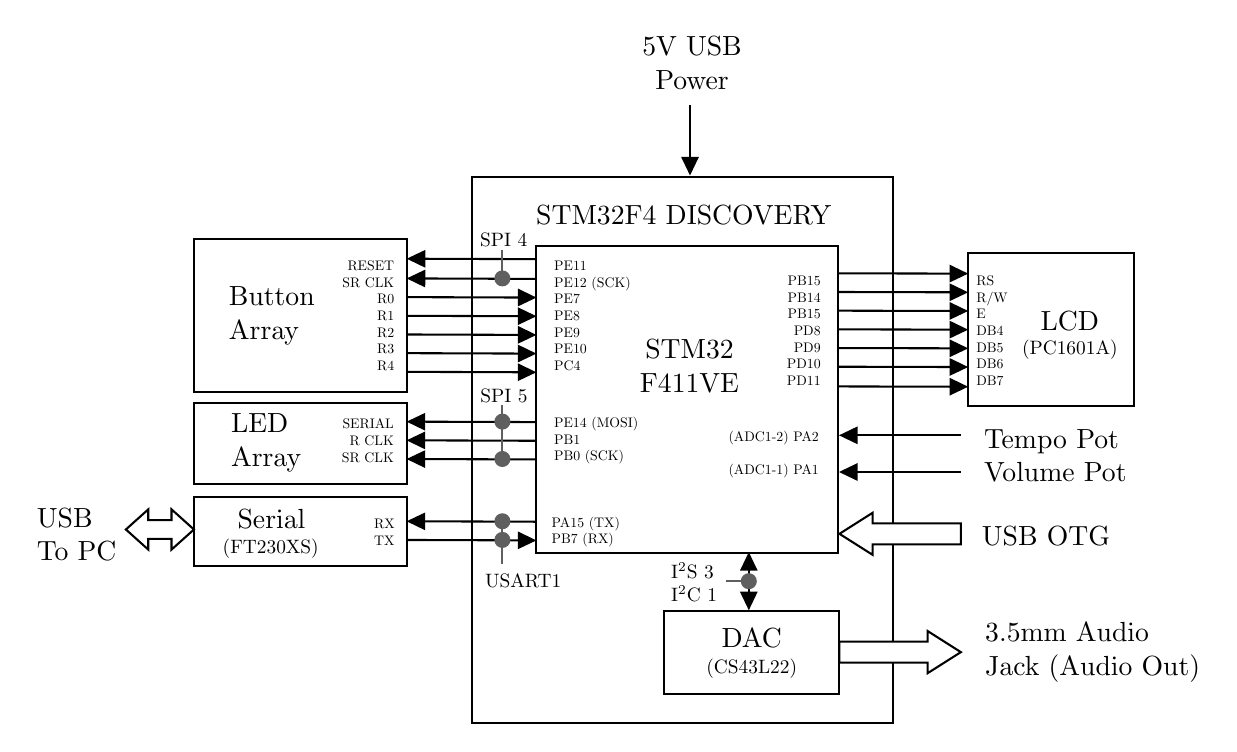
\begin{tikzpicture}[x=0.75pt,y=0.75pt,yscale=-1,xscale=1]
	%uncomment if require: \path (0,481); %set diagram left start at 0, and has height of 481
	
	%Shape: Rectangle [id:dp5918076160842385] 
	\draw   (230,97) -- (433,97) -- (433,360) -- (230,360) -- cycle ;
	%Shape: Rectangle [id:dp0432000596696005] 
	\draw   (322.5,306) -- (406.98,306) -- (406.98,346) -- (322.5,346) -- cycle ;
	%Shape: Rectangle [id:dp7985098815357947] 
	\draw   (261,130) -- (406.5,130) -- (406.5,278) -- (261,278) -- cycle ;
	%Right Arrow [id:dp2315359222828235] 
	\draw  [fill={rgb, 255:red, 255; green, 255; blue, 255 }  ,fill opacity=1 ] (407,320.79) -- (449.5,320.79) -- (449.5,315.71) -- (465.5,325.86) -- (449.5,336) -- (449.5,330.93) -- (407,330.93) -- cycle ;
	%Straight Lines [id:da20381712216745096] 
	\draw    (363.33,279.7) -- (363.33,303.67) ;
	\draw [shift={(363.33,305.67)}, rotate = 270] [fill={rgb, 255:red, 0; green, 0; blue, 0 }  ][line width=0.75]  [draw opacity=0] (8.93,-4.29) -- (0,0) -- (8.93,4.29) -- cycle    ;
	\draw [shift={(363.33,277.7)}, rotate = 90] [fill={rgb, 255:red, 0; green, 0; blue, 0 }  ][line width=0.75]  [draw opacity=0] (8.93,-4.29) -- (0,0) -- (8.93,4.29) -- cycle    ;
	%Right Arrow [id:dp9428678654929861] 
	\draw  [fill={rgb, 255:red, 255; green, 255; blue, 255 }  ,fill opacity=1 ] (465.5,273.93) -- (423,273.93) -- (423,279) -- (407,268.86) -- (423,258.71) -- (423,263.79) -- (465.5,263.79) -- cycle ;
	%Straight Lines [id:da6753000057653133] 
	\draw    (465.5,239.07) -- (408.8,239.07) ;
	\draw [shift={(406.8,239.07)}, rotate = 360] [fill={rgb, 255:red, 0; green, 0; blue, 0 }  ][line width=0.75]  [draw opacity=0] (8.93,-4.29) -- (0,0) -- (8.93,4.29) -- cycle    ;
	
	%Straight Lines [id:da7619363353708244] 
	\draw [color={rgb, 255:red, 0; green, 0; blue, 0 }  ,draw opacity=1 ]   (465.5,221.4) -- (408.8,221.4) ;
	\draw [shift={(406.8,221.4)}, rotate = 360] [fill={rgb, 255:red, 0; green, 0; blue, 0 }  ,fill opacity=1 ][line width=0.75]  [draw opacity=0] (8.93,-4.29) -- (0,0) -- (8.93,4.29) -- cycle    ;
	
	%Straight Lines [id:da15096112605281875] 
	\draw    (406.5,188.35) -- (467,188.5) ;
	\draw [shift={(469,188.5)}, rotate = 180.14] [fill={rgb, 255:red, 0; green, 0; blue, 0 }  ][line width=0.75]  [draw opacity=0] (8.93,-4.29) -- (0,0) -- (8.93,4.29) -- cycle    ;
	
	%Straight Lines [id:da6435790607323693] 
	\draw    (406.5,179.35) -- (467,179.5) ;
	\draw [shift={(469,179.5)}, rotate = 180.14] [fill={rgb, 255:red, 0; green, 0; blue, 0 }  ][line width=0.75]  [draw opacity=0] (8.93,-4.29) -- (0,0) -- (8.93,4.29) -- cycle    ;
	
	%Straight Lines [id:da7889393535599036] 
	\draw    (406.5,170.35) -- (467,170.5) ;
	\draw [shift={(469,170.5)}, rotate = 180.14] [fill={rgb, 255:red, 0; green, 0; blue, 0 }  ][line width=0.75]  [draw opacity=0] (8.93,-4.29) -- (0,0) -- (8.93,4.29) -- cycle    ;
	
	%Straight Lines [id:da6837607975654587] 
	\draw    (406.5,161.35) -- (467,161.5) ;
	\draw [shift={(469,161.5)}, rotate = 180.14] [fill={rgb, 255:red, 0; green, 0; blue, 0 }  ][line width=0.75]  [draw opacity=0] (8.93,-4.29) -- (0,0) -- (8.93,4.29) -- cycle    ;
	
	%Straight Lines [id:da865188420352889] 
	\draw    (406.5,152.35) -- (467,152.5) ;
	\draw [shift={(469,152.5)}, rotate = 180.14] [fill={rgb, 255:red, 0; green, 0; blue, 0 }  ][line width=0.75]  [draw opacity=0] (8.93,-4.29) -- (0,0) -- (8.93,4.29) -- cycle    ;
	
	%Straight Lines [id:da2449046730837665] 
	\draw    (406.5,143.35) -- (467,143.5) ;
	\draw [shift={(469,143.5)}, rotate = 180.14] [fill={rgb, 255:red, 0; green, 0; blue, 0 }  ][line width=0.75]  [draw opacity=0] (8.93,-4.29) -- (0,0) -- (8.93,4.29) -- cycle    ;
	
	%Straight Lines [id:da2794456064676478] 
	\draw    (406.5,197.85) -- (467,198) ;
	\draw [shift={(469,198)}, rotate = 180.14] [fill={rgb, 255:red, 0; green, 0; blue, 0 }  ][line width=0.75]  [draw opacity=0] (8.93,-4.29) -- (0,0) -- (8.93,4.29) -- cycle    ;
	
	%Shape: Rectangle [id:dp2417461204409681] 
	\draw   (469,133.57) -- (549,133.57) -- (549,207.23) -- (469,207.23) -- cycle ;
	%Straight Lines [id:da008963581922469599] 
	\draw    (261.02,146.03) -- (200.52,145.82) ;
	\draw [shift={(198.52,145.82)}, rotate = 360.2] [fill={rgb, 255:red, 0; green, 0; blue, 0 }  ][line width=0.75]  [draw opacity=0] (8.93,-4.29) -- (0,0) -- (8.93,4.29) -- cycle    ;
	
	%Straight Lines [id:da7017501912001678] 
	\draw    (259.01,155.03) -- (198.51,154.82) ;
	
	\draw [shift={(261.01,155.03)}, rotate = 180.2] [fill={rgb, 255:red, 0; green, 0; blue, 0 }  ][line width=0.75]  [draw opacity=0] (8.93,-4.29) -- (0,0) -- (8.93,4.29) -- cycle    ;
	%Straight Lines [id:da6133179873808812] 
	\draw    (259,164.03) -- (198.5,163.82) ;
	
	\draw [shift={(261,164.03)}, rotate = 180.2] [fill={rgb, 255:red, 0; green, 0; blue, 0 }  ][line width=0.75]  [draw opacity=0] (8.93,-4.29) -- (0,0) -- (8.93,4.29) -- cycle    ;
	%Straight Lines [id:da38787523560372406] 
	\draw    (258.99,173.03) -- (198.49,172.82) ;
	
	\draw [shift={(260.99,173.03)}, rotate = 180.2] [fill={rgb, 255:red, 0; green, 0; blue, 0 }  ][line width=0.75]  [draw opacity=0] (8.93,-4.29) -- (0,0) -- (8.93,4.29) -- cycle    ;
	%Straight Lines [id:da049319380388482825] 
	\draw    (258.98,182.03) -- (198.48,181.82) ;
	
	\draw [shift={(260.98,182.03)}, rotate = 180.2] [fill={rgb, 255:red, 0; green, 0; blue, 0 }  ][line width=0.75]  [draw opacity=0] (8.93,-4.29) -- (0,0) -- (8.93,4.29) -- cycle    ;
	%Straight Lines [id:da747407414364454] 
	\draw    (258.97,191.03) -- (198.47,190.82) ;
	
	\draw [shift={(260.97,191.03)}, rotate = 180.2] [fill={rgb, 255:red, 0; green, 0; blue, 0 }  ][line width=0.75]  [draw opacity=0] (8.93,-4.29) -- (0,0) -- (8.93,4.29) -- cycle    ;
	%Straight Lines [id:da5651387140870967] 
	\draw    (261.03,136.53) -- (200.53,136.32) ;
	\draw [shift={(198.53,136.32)}, rotate = 360.2] [fill={rgb, 255:red, 0; green, 0; blue, 0 }  ][line width=0.75]  [draw opacity=0] (8.93,-4.29) -- (0,0) -- (8.93,4.29) -- cycle    ;
	
	%Shape: Rectangle [id:dp8694052933297145] 
	\draw   (96.2,126.97) -- (198.5,126.97) -- (198.5,200.63) -- (96.2,200.63) -- cycle ;
	%Straight Lines [id:da2504593501522252] 
	\draw    (260.98,263.03) -- (200.48,262.82) ;
	\draw [shift={(198.48,262.82)}, rotate = 360.2] [fill={rgb, 255:red, 0; green, 0; blue, 0 }  ][line width=0.75]  [draw opacity=0] (8.93,-4.29) -- (0,0) -- (8.93,4.29) -- cycle    ;
	
	%Straight Lines [id:da13433373243842728] 
	\draw    (258.97,272.03) -- (198.47,271.82) ;
	
	\draw [shift={(260.97,272.03)}, rotate = 180.2] [fill={rgb, 255:red, 0; green, 0; blue, 0 }  ][line width=0.75]  [draw opacity=0] (8.93,-4.29) -- (0,0) -- (8.93,4.29) -- cycle    ;
	%Shape: Rectangle [id:dp8665495313374194] 
	\draw   (96.2,251) -- (198.5,251) -- (198.5,284.2) -- (96.2,284.2) -- cycle ;
	%Straight Lines [id:da01047939684415633] 
	\draw    (260.99,215.03) -- (200.49,214.82) ;
	\draw [shift={(198.49,214.82)}, rotate = 360.2] [fill={rgb, 255:red, 0; green, 0; blue, 0 }  ][line width=0.75]  [draw opacity=0] (8.93,-4.29) -- (0,0) -- (8.93,4.29) -- cycle    ;
	
	%Straight Lines [id:da30157272917946076] 
	\draw    (260.98,224.03) -- (200.48,223.82) ;
	\draw [shift={(198.48,223.82)}, rotate = 360.2] [fill={rgb, 255:red, 0; green, 0; blue, 0 }  ][line width=0.75]  [draw opacity=0] (8.93,-4.29) -- (0,0) -- (8.93,4.29) -- cycle    ;
	
	%Straight Lines [id:da6459450622816814] 
	\draw    (260.97,233.03) -- (200.47,232.82) ;
	\draw [shift={(198.47,232.82)}, rotate = 360.2] [fill={rgb, 255:red, 0; green, 0; blue, 0 }  ][line width=0.75]  [draw opacity=0] (8.93,-4.29) -- (0,0) -- (8.93,4.29) -- cycle    ;
	
	%Shape: Rectangle [id:dp9252289543251917] 
	\draw   (96.2,205.88) -- (198.47,205.88) -- (198.47,244.98) -- (96.2,244.98) -- cycle ;
	%Left Right Arrow [id:dp964472909485768] 
	\draw   (63.2,266.77) -- (74,257.08) -- (74,262.28) -- (85.2,262.28) -- (85.2,257.08) -- (96,266.77) -- (85.2,276.46) -- (85.2,271.26) -- (74,271.26) -- (74,276.46) -- cycle ;
	%Straight Lines [id:da39718515123626186] 
	\draw    (335,62.2) -- (335,94.2) ;
	\draw [shift={(335,96.2)}, rotate = 270] [fill={rgb, 255:red, 0; green, 0; blue, 0 }  ][line width=0.75]  [draw opacity=0] (8.93,-4.29) -- (0,0) -- (8.93,4.29) -- cycle    ;
	
	%Straight Lines [id:da06860468568514189] 
	\draw [color={rgb, 255:red, 95; green, 95; blue, 95 }  ,draw opacity=1 ][line width=0.75]    (244.6,132.18) -- (244.6,145.8) ;
	\draw [shift={(244.6,145.8)}, rotate = 90] [color={rgb, 255:red, 95; green, 95; blue, 95 }  ,draw opacity=1 ][fill={rgb, 255:red, 95; green, 95; blue, 95 }  ,fill opacity=1 ][line width=0.75]      (0, 0) circle [x radius= 3.35, y radius= 3.35]   ;
	
	%Straight Lines [id:da4751452819167077] 
	\draw [color={rgb, 255:red, 95; green, 95; blue, 95 }  ,draw opacity=1 ]   (244.6,208.58) -- (244.6,232.8) ;
	\draw [shift={(244.6,232.8)}, rotate = 90] [color={rgb, 255:red, 95; green, 95; blue, 95 }  ,draw opacity=1 ][fill={rgb, 255:red, 95; green, 95; blue, 95 }  ,fill opacity=1 ][line width=0.75]      (0, 0) circle [x radius= 3.35, y radius= 3.35]   ;
	
	%Straight Lines [id:da9004528527180191] 
	\draw [color={rgb, 255:red, 95; green, 95; blue, 95 }  ,draw opacity=1 ]   (244.6,207.03) -- (244.6,214.8) ;
	\draw [shift={(244.6,214.8)}, rotate = 90] [color={rgb, 255:red, 95; green, 95; blue, 95 }  ,draw opacity=1 ][fill={rgb, 255:red, 95; green, 95; blue, 95 }  ,fill opacity=1 ][line width=0.75]      (0, 0) circle [x radius= 3.35, y radius= 3.35]   ;
	
	%Straight Lines [id:da4193219413571099] 
	\draw [color={rgb, 255:red, 95; green, 95; blue, 95 }  ,draw opacity=1 ][line width=0.75]    (352.25,291.68) -- (363.33,291.68) ;
	\draw [shift={(363.33,291.68)}, rotate = 0] [color={rgb, 255:red, 95; green, 95; blue, 95 }  ,draw opacity=1 ][fill={rgb, 255:red, 95; green, 95; blue, 95 }  ,fill opacity=1 ][line width=0.75]      (0, 0) circle [x radius= 3.35, y radius= 3.35]   ;
	
	%Straight Lines [id:da9875335917540662] 
	\draw [color={rgb, 255:red, 95; green, 95; blue, 95 }  ,draw opacity=1 ]   (244.6,283.3) -- (244.6,262.8) ;
	\draw [shift={(244.6,262.8)}, rotate = 270] [color={rgb, 255:red, 95; green, 95; blue, 95 }  ,draw opacity=1 ][fill={rgb, 255:red, 95; green, 95; blue, 95 }  ,fill opacity=1 ][line width=0.75]      (0, 0) circle [x radius= 3.35, y radius= 3.35]   ;
	
	%Straight Lines [id:da32970854077013634] 
	\draw [color={rgb, 255:red, 95; green, 95; blue, 95 }  ,draw opacity=1 ]   (244.6,283.3) -- (244.6,271.8) ;
	\draw [shift={(244.6,271.8)}, rotate = 270] [color={rgb, 255:red, 95; green, 95; blue, 95 }  ,draw opacity=1 ][fill={rgb, 255:red, 95; green, 95; blue, 95 }  ,fill opacity=1 ][line width=0.75]      (0, 0) circle [x radius= 3.35, y radius= 3.35]   ;
	
	
	% Text Node
	\draw (332,115.5) node  [align=center] {STM32F4 DISCOVERY};
	% Text Node
	\draw (336,42) node  [align=center] {5V USB \\Power};
	% Text Node
	\draw (364.74,319) node  [align=left] {DAC};
	% Text Node
	\draw (334.75,188) node  [align=center] {STM32\\F411VE};
	% Text Node
	\draw (529,326) node  [align=left] {3.5mm Audio\\Jack (Audio Out)};
	% Text Node
	\draw (506.5,270) node  [align=left] {USB OTG};
	% Text Node
	\draw (511,231) node  [align=left] {Tempo Pot\\Volume Pot};
	% Text Node
	\draw (518,166.4) node  [align=left] {LCD};
	% Text Node
	\draw (480.5,171) node [scale=0.5] [align=left] {RS\\R/W\\E\\DB4\\DB5\\DB6\\DB7};
	% Text Node
	\draw (389.83,171) node [scale=0.5] [align=right] {PB15\\PB14\\PB15\\PD8\\PD9\\PD10\\PD11};
	% Text Node
	\draw (375.33,230.5) node [scale=0.5] [align=right] {(ADC1-2) PA2\\\\(ADC1-1) PA1};
	% Text Node
	\draw (133.5,163.8) node  [align=left] {Button\\Array};
	% Text Node
	\draw (180,163.8) node [scale=0.5] [align=right] {RESET\\SR CLK\\R0\\R1\\R2\\R3\\R4};
	% Text Node
	\draw (288,163.8) node [scale=0.5] [align=left] {PE11\\PE12 (SCK)\\PE7\\PE8\\PE9\\PE10\\PC4};
	% Text Node
	\draw (133.35,261.6) node  [align=left] {Serial};
	% Text Node
	\draw (284.8,268) node [scale=0.5] [align=left] {PA15 (TX)\\PB7 (RX)};
	% Text Node
	\draw (187.8,268) node [scale=0.5] [align=left] {RX\\TX};
	% Text Node
	\draw (179.8,224) node [scale=0.5] [align=right] {SERIAL\\R CLK\\SR CLK};
	% Text Node
	\draw (130.75,225) node  [align=left] {LED\\Array};
	% Text Node
	\draw (289.8,224) node [scale=0.5] [align=left] {PE14 (MOSI)\\PB1\\PB0 (SCK)};
	% Text Node
	\draw (133,276) node [scale=0.7] [align=left] {(FT230XS)};
	% Text Node
	\draw (39.5,269.35) node  [align=left] {USB\\To PC};
	% Text Node
	\draw (518,180) node [scale=0.7] [align=left] {(PC1601A)};
	% Text Node
	\draw (337,292) node [scale=0.7] [align=left] {I$^2$S 3\\I$^2$C 1};
	% Text Node
	\draw (245.22,127.31) node [scale=0.7] [align=left] {SPI 4};
	% Text Node
	\draw (245.36,202.61) node [scale=0.7] [align=left] {SPI 5};
	% Text Node
	\draw (364.74,334) node [scale=0.7] [align=left] {(CS43L22)};
	% Text Node
	\draw (254.6,291.3) node [scale=0.7] [align=left] {USART1};
	\end{tikzpicture}
	\caption{Complete System Diagram}
	\label{fig:sysDiag}
\end{figure}
\noindent Figure \ref{fig:sysDiag} shows the complete system diagram, however, it should be noted that there are portions of the STM32F411 Discovery board not shown due to them not being used. An example of this would be the included onboard MEMS microphone \cite{f411brd}. This figure shows where the bounds of each sub-section of the completed system are and their means of communication. 

%----------------------------------------------------------------------------------------
%	SECTION 4
%----------------------------------------------------------------------------------------
\chapter{Software Design}
\section{Main Software Loop}
\begin{figure}[h!]
	\centering
	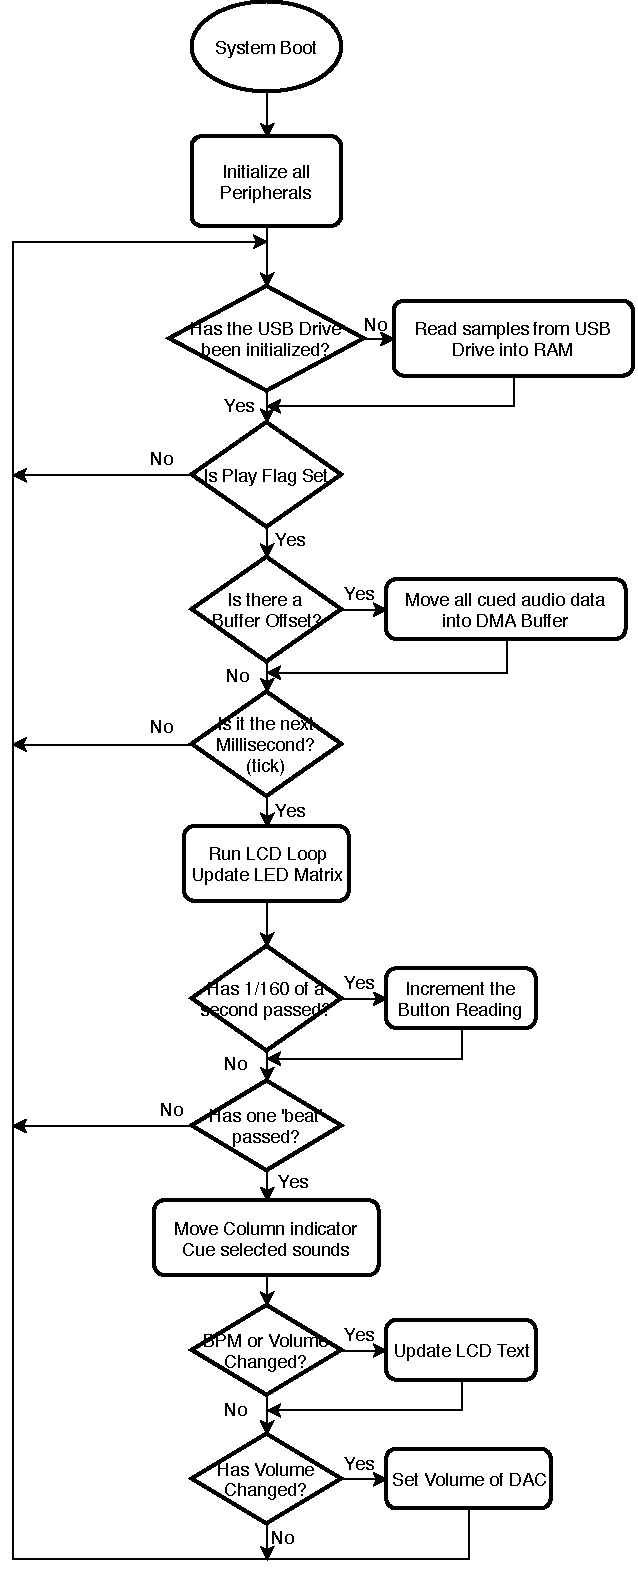
\includegraphics[height = 0.62 \textheight, angle=0, origin=c]{NewFullSystemDiagram.pdf}
	\caption{Full System Software Flow Diagram}
	\label{fig:SysFlowDiag}
\end{figure}
\noindent When the \ac{uc} begins to run the code there are two stages. Firstly there is the initialization stage where all code that must only happen once is run. The code here includes all the peripheral initialization and some variable manipulation and initialization. After this stage, an infinite loop begins. In this loop, all code to control the peripherals and subsystems is found. The \ac{uc} will step through all the code in the loop and then it will begin back at the beginning of the loop. Several flags will need to be set to allow for conditional functions. The \ac{uc} will run this code as fast as it possibly can, thus, seeing as a consistent time between certain functions is needed, a system tick (sysTick) will update every millisecond. This millisecond clock can then be used to see if a certain amount of time has passed and thus cause desired functions to run. As the \ac{uc} runs faster than its one-millisecond timer a semi-asynchronous function can be run. This can be seen when the \ac{uc} updates the audio buffer as soon as a flag is set. Efforts have been made to cut out functions that would run repetitively unnecessary, for example, the updating of the \ac{lcd} text.\\
This chapter will discuss each of the major sub-sections' software implementation on the \ac{uc}. 
\section{LED and Button Matrix Control}
\subsection{Setting LEDs}
\subsubsection{Updating the Driver ICs}
Several variables are used to store the current \ac{led} states and use them to drive the \ac{led} matrix. To store the value of each row there is an array of 16-bit integers. Each integer in the array holds the values of the led in the corresponding row, so if the first and third \ac{led} in row zero is enabled the integer would be $(1010\ 0000)_2$. This variable is named cData. When sending data over the \ac{spi} protocol only one column at a time is selected. A tracker for the columns must be in place that increments often enough to create a believable persistence.
\begin{lstlisting}[language=C, caption=Driving a row of LEDs, captionpos = b, numbers=left, frame=single,tabsize=3, label={lst:ledspi}]
spiData[0] = (0x8000 >> c) & 0x00FF;
spiData[1] = ((0x8000 >> c) & 0xFF00) >> 8;
spiData[2] = 0;
for (uint8_t r = 0; r < 5; r++){
	spiData[2] |= (((cData[r] & (0x8000 >> c)) << c ) >> (r+8));
}

HAL_GPIO_WritePin(GPIOB, GPIO_PIN_1, GPIO_PIN_RESET);
HAL_SPI_Transmit(&hspi5, spiData, 3, 10);
HAL_GPIO_WritePin(GPIOB, GPIO_PIN_1, GPIO_PIN_SET);
\end{lstlisting}
In Listing \ref{lst:ledspi} the code used to drive the \ac{led} matrix can be seen. Lines one and two are selecting the current column (c) by shifting $(1000\ 0000\ 0000\ 0000)_2$ right by the column number to pull high the chosen column physically. That value is then masked and shifted to split the 16-bit integer into two eight bit integers. Lines three through six step over each row and modify the row variable. Each column variable is checked if the value is high or low at the specific column and it is placed from the eighth to the third bit of the row variable (spiData[2]). If the first and fifth row is high in the selected column the result would be $(1000\ 1000)_2$.\\
Lines eight through ten set the RCLK pin low, transfer the data, and sets RCLK high again. The data transferred is spiData which is three bits long. As the shift registers are connected to the rows, the low columns and then the high columns the data must be transmitted in reverse: high columns, low columns, and then rows - hence spiData is placed in this order. SPI5 is used for this transfer in the Motorola Frame Format that is eight bits long and the least significant bit is sent first.
\subsubsection{Changing the State Variable}
To change the state of any \ac{led} at any time a simple toggle of a bit in cData can be used. The desired row's cData element is selected and is then XOR'ed with $(0001)_2$ shifted left $15-c$, where c is the desired column \cite{xor}.
\subsubsection{Incrementing the Indicator Column}
As time passes the indicator column must move on to the next column at a certain interval. The time is decided by the \ac{bpm} value calculated in Section \ref{sec:adcSoft}. Toggling of the \acap{led} in the required columns is quite simple. A loop will go over each row and toggle the \acap{led} in the required column. This can then be done twice, once to the new column and once to the current as this will revert the \acap{led} back to how they were before selection. If the next column is zero then the current will be column fifteen.
\subsection{Reading a column of buttons}
\subsubsection{Reading the Selected Column}
To drive the decade counter circuit being used for the column select a single clock input must be provided. To allow for actions to happen between each clock cycle a custom clock is used rather than one generated by the \ac{uc} itself. To emulate this clock signal the corresponding \ac{gpio} pin will be toggled high and then low. Once the clock is toggled the selected column tracking variable will increment, or reset to zero if the value becomes sixteen. A two-dimensional array is kept with the previous state of each button.\\
A loop goes over each row and checks if the new state of the button does not match that of the prior. When this is the case the \ac{led} in that location will be toggled if the button is being pressed, not released. If the two states did not match the previous will be updated to match the current state.
\subsubsection{Resetting the Button Matrix}
Resetting the button matrix is made incredibly simple thanks to the decade counter circuit being used. This system allows for the Reset line to be pulled high resulting in all outputs going low and the position being reset. In the software, the selected column tracker variable must be set back to zero as well.
\section{LCD with Tempo and Volume Control}
\subsection{LCD}
The code for the \ac{lcd} was adapted from a file supplied by Dr. L. Visagie designed for the STM32F344R8 Nucleo Board. 
\subsubsection{Sending Data}
To send data to the LCD one nibble must be sent at a time as only four lines are in place. This decision was made to reduce the pin count to the \ac{uc}. To send data to the \ac{lcd} the Enable (E), and Read not Write (RNW) pins must be pulled low. The Register Select (RS) pin must be set to the appropriate state, low for commands or high for data. Just before the data is sent the Enable pin is pulled high and is kept that way until the nibble has been sent. Now the data nibble must be transmitted in parallel over DB4 through DB7. \\
To send a byte of data, rather than a nibble, the byte must be split in two. This can be achieved with masking and shifting. The high nibble must be sent first then only the low nibble. The controller on the \ac{lcd} will reassemble the data as needed. Between each nibble being pushed a short delay must take place to ensure the correct separation of the data.
\subsubsection{LCD Finite State Machine}
\begin{table}[h!]
	\centering
	\begin{tabular}{ | r |  p{2.7cm}| p{2.7cm}| p{2.5cm} | l | }
		\hline
		\multicolumn{1}{|l|}{\textbf{State}} & \textbf{1st Nibble \newline (RS, Nibble)} & \textbf{2nd Nibble\newline (RS, Nibble)} & \textbf{Time Delay \newline after (ms)} & \textbf{Description} \\ \hline
		0 & - & - & - & Idle \\ \hline
		1 & 0,3 & - & 5 &  \\ \hline
		2 & 0,3 & - & 1 &  \\ \hline
		3 & 0,3 & - & 1 &  \\ \hline
		4 & 0,2 & - & 1 & 4 bit mode \\ \hline
		5 & 0,2 & 0,8 & 1 & 4 bit mode 2 line \\ \hline
		6 & 0,0 & 0,14 & 1 & Display On Cursor Off \\ \hline
		7 & 0,0 & 0,1 & 1 & Clear Display \\ \hline
		8 & 0,0 & 0,6 & 1 & Increment Cursor \\ \hline
		9 & 0,8 & 0,0 & 1 & Home \\ \hline
		10 & - & - & 100 &  \\ \hline
		20 & 0,8 & 0,0 & 3 & Home \\ \hline
		21 & \multicolumn{2}{c|}{Push Data Byte }  & - &  \\ \hline
	\end{tabular}
	\caption{LCD Initialization and Run State Machine}
	\label{tab:LCDfsm}
\end{table}
\noindent Table \ref{tab:LCDfsm} shows the states of the \ac{fsm} used to initialize and run the \ac{lcd}. To initialize the display states one through ten must be run. Every state will cue the next state upon completion. Each of these states will send one or two nibbles using the method mentioned before. After the data is transmitted a delay, in milliseconds, must occur for the \ac{lcd} to process the data sent. A description of the commands sent is also shown in Table \ref{tab:LCDfsm}. These states will only be called once when the \ac{uc} is first started up. The state variable will not be set to one again after state ten has been completed\\
States twenty and twenty-one are in place to reset the cursor location and send a byte of data respectively. The data byte is sent using the code for sending a byte of data discussed prior. When the data for the display is updated the state will be set to twenty so that this procedure runs.\\
State zero is in place as an idle marker. This is used to indicate when nothing must be done to the display. Calling this state is done once all other states in the \ac{fsm} have been completed. A simple check before the \ac{fsm}'s switch statement allows the update of the time tracking feature to be skipped entirely. Note that this means that this state is separate from the rest of the finite state machine and thus does not progress on its own, the state must be manually changed.
\subsubsection{Display Data}
When writing the data to the \ac{lcd} two loops are used to fill the first and second half of the display. This is done as the display stores the first and last eight characters from separate locations in \ac{ram}. Between the two loops, a command is used to shift the location of where data is being written. The command used for this transmitting a command byte: RS is low and The data is $(192)_{10}$ \cite{lcd}.
\begin{figure}[h!]
	\centering
	\begin{tabular}{|c|c|c|c|c|c|c|c||c|c|c|c|c|c|c|c|}
		\hline
		$x$ & $y$ & $z$ & \  &B & P & M & \  & V & o & l & : & $a$ & $b$ & $c$ & $d$ \\
		\hline
		\multicolumn{8}{|c||}{\textit{BPMString}} & \multicolumn{8}{c|}{\textit{VolString}}\\
		\hline
	\end{tabular}
	\caption{The data format of the LCD}
	\label{fig:LCDDat}
\end{figure}\\
The data being pushed is placed in two arrays from another function separate to the \ac{fsm}. This function takes in two integers, the \ac{bpm} and volume values calculated using the \ac{adc} values. The format of the display is shown in Figure \ref{fig:LCDDat}. Values $x$, $y$, and $z$ are the \ac{bpm} value as calculated from the \ac{adc}. Values $a$ through $d$ are the volume values, this is formatted as '$nnn\%$' when non-zero or 'Mute' when the volume is zero percent. For both of these cases, if the leading integers are zero they will be replaced with a space character rather than zero. The strings, or character arrays, are made sure to have a length of eight to ensure there is no misalignment of data or unwanted data being read. At the end of the function, the next state is set to twenty to write the new data to the \ac{lcd}.
\subsection{ADC Calculations} \label{sec:adcSoft}
\subsubsection{Direct Memory Access} \label{sec:dma}
\ac{dma} is used by multiple features on the \ac{uc} to reduce the workload of the \ac{cpu}. \ac{dma} transfers a given array's data to a peripheral or from a peripheral into a variable without using \ac{cpu} cycles. This can be set up to transfer in various lengths: byte, half-word, and word. Furthermore, the \ac{dma} can be set up to run linearly or circularly, this means that when the end of the buffer is reached it will either stop or restart reading respectively \cite{f411}. 
\begin{figure}[h!]
	\centering
	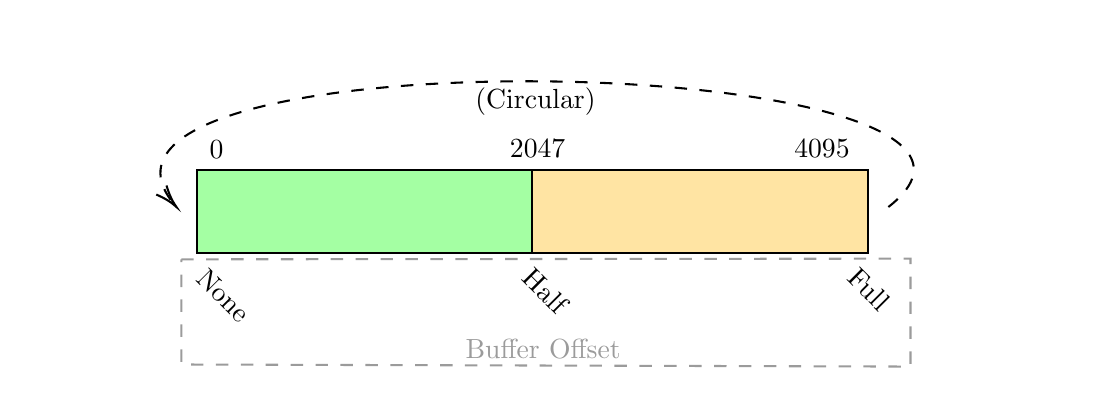
\begin{tikzpicture}[x=0.75pt,y=0.75pt,yscale=-1,xscale=1]
	%uncomment if require: \path (0,300); %set diagram left start at 0, and has height of 300
	
	%Shape: Rectangle [id:dp4990118466714293] 
	\draw  [fill={rgb, 255:red, 164; green, 255; blue, 163 }  ,fill opacity=1 ] (124,111) -- (285.5,111) -- (285.5,151) -- (124,151) -- cycle ;
	%Shape: Rectangle [id:dp25755731593996956] 
	\draw  [fill={rgb, 255:red, 255; green, 228; blue, 163 }  ,fill opacity=1 ] (285.5,111) -- (447,111) -- (447,151) -- (285.5,151) -- cycle ;
	%Curve Lines [id:da23888848228530857] 
	\draw  [dash pattern={on 4.5pt off 4.5pt}]  (457,129) .. controls (553.85,54.04) and (42.82,43.11) .. (112.9,127.72) ;
	\draw [shift={(114,129)}, rotate = 228.41] [color={rgb, 255:red, 0; green, 0; blue, 0 }  ][line width=0.75]    (10.93,-3.29) .. controls (6.95,-1.4) and (3.31,-0.3) .. (0,0) .. controls (3.31,0.3) and (6.95,1.4) .. (10.93,3.29)   ;
	
	%Shape: Polygon [id:ds7142067873406877] 
	\draw  [color={rgb, 255:red, 155; green, 155; blue, 155 }  ,draw opacity=1 ][dash pattern={on 4.5pt off 4.5pt}] (116.33,154.22) -- (467.67,153.89) -- (467.67,205.89) -- (116.33,204.89) -- (116.33,154.22) -- cycle ;
	
	% Text Node
	\draw (136.67,171.67) node [rotate=-45] [align=left] {None};
	% Text Node
	\draw (291.67,169.33) node [rotate=-45] [align=left] {Half};
	% Text Node
	\draw (447.67,168.67) node [rotate=-45] [align=left] {Full};
	% Text Node
	\draw (287,78) node  [align=left] {(Circular)};
	% Text Node
	\draw (133.33,101.17) node  [align=left] {0};
	% Text Node
	\draw (288,100.67) node  [align=left] {2047};
	% Text Node
	\draw (425,100.67) node  [align=left] {4095};
	% Text Node
	\draw (290.67,197.33) node [color={rgb, 255:red, 155; green, 155; blue, 155 }  ,opacity=1 ] [align=left] {Buffer Offset};
	\end{tikzpicture}
	\caption{DMA Buffer Example}
	\label{fig:dma}
\end{figure}\\
Figure \ref{fig:dma} aids in explaining further concepts. This figure shows an example where the length of the buffer is 4096 samples and data is coming from the \ac{uc} going to a peripheral. As the data is read from the buffer there are two callbacks that will occur. These are when the data read is halfway and when it has completed. In each case there will be a flag updated, the buffer offset, to reflect the current position. This flag can be used to start replacing data in the opposite half of the buffer when in circular mode. This implies that when the Half buffer offset is set the first, green, half of the buffer can get the data following on from the end of the second, orange, half. \\
\ac{dma} is used for the \ac{adc} readings. Once the transfer to the array of data coming from the \ac{adc} is complete the values in this buffer are moved into another array. This is done to prevent reading and writing to the same array location simultaneously resulting in corrupted data. These values from the second array are then used by the rest of the code. The \ac{dma} channel for the \ac{adc} is set up in circular mode transferring a full word. The full word is needed as the \ac{adc} is set up in 12-bit mode. As there are two channels of the \ac{adc} in use the two values will be placed consecutively in the desired array.
\subsubsection{Manipulation of ADC Values}
The two \ac{adc} channels measure the voltage from the two voltage divider circuits discussed prior. One channel will be used for the tempo measurement and the other for the master volume. The tempo measurement will be used to determine not only the \ac{bpm} but also the milliseconds per beat. The latter of these is compared to the number of sysTicks from the previous update. sysTick is a timer integer that is incremented every millisecond. An integer is used to count a number of ticks until it is reset. 
\begin{equation}
\label{eqn:mspb}
\begin{aligned}
\text{mSPB} &= 1000 * \frac{4096 - \text{ADC}}{4095}
\end{aligned}
\end{equation}
Equation \ref{eqn:mspb} shows the formula being used to determine when to run the matrix updating code as well as resetting the tick counter. In this equation, the 1000 is in place as this is how many ticks are in one second \cite{f411}. The \ac{adc} value is subtracted from the maximal 12-bit value ($2^{12} = 4096$) and then divided by the same maximal value minus one. The reason for subtracting the \ac{adc} value from the maximum is due to the value read by the \ac{adc} being inversely proportional to the time taken to refresh, hence when the voltage divider is at its maximum value the time between each update should be at its minimum.\\
Once the matrix update code runs there are two more values required for the \ac{lcd}. These are the \ac{bpm} value and volume. To determine the \ac{bpm} a similar equation to Equation \ref{eqn:mspb} is needed. 
\begin{equation}
	\label{eqn:bpm}
	\begin{aligned}
	\text{BPM} &= 60 * \frac{4095}{4096 - \text{ADC}}
	\end{aligned}
\end{equation}
Equation \ref{eqn:bpm} is the formula used for this exact purpose. This formula inverts the fraction from the mSPB formula as now it is beats per time instead of the other way around. The value of the \ac{adc} is at most 4095, thus subtracting this from 4096 will never result in dividing by zero. The sixty in the formula is there as there are sixty seconds in a minute, as is needed for \acl{bpm}. If the value of the voltage divider is at a maximum, the \ac{bpm} value will also be at its maximum. 
\begin{equation}
	\label{eqn:vol}
\begin{aligned}
\text{VOL} &= 100*\frac{\text{ADC}}{4095}
\end{aligned}
\end{equation}
To determine the volume a simple percentage equation is used. Equation \ref{eqn:vol} shows exactly this. This \ac{adc} channel is also 12-bit, hence to get a fraction of the maximal value (4095) the measured value is simply divided by the maximum. To convert a fraction into a percentage value the fraction must be multiplied by one hundred. This outputs a value between zero and one hundred, exactly what is desired for a percentage value.
\section{Audio File Reading and Playback} \label{sec:audioSetup}
\subsection{The WAV file format} \label{sec:waveformat}
To have a better understanding of what the \ac{uc} must interpret when reading a .wav file the header of such a file must be understood as well as the basic structure. The wave format is a type of \ac{riff} file with a single WAVE chunk \cite{wave}. The WAVE chunk has two sub-chunks, 'fmt ' and 'data'. These contain the data format information and audio data respectively \cite{wave}.
\begin{table}[h!]
	\centering
	\begin{tabular}{ | l | l | l | l | p{7.5cm} | }
		\hline 
		\textbf{Pos.} & \textbf{Size} & \textbf{Endian} & \textbf{Field Name} & \textbf{Data in this Position} \\ \hline
		0 & 4 & big & ChunkID & "RIFF" \\ \hline
		4 & 4 & little & ChunkSize & 4 + (8 + SubChunk1Size) + (8 + SubChunk2Size) \\ \hline
		8 & 4 & big & Format & "WAVE" \\ \hline
		12 & 4 & big & SubChunk1ID & "fmt " \\ \hline
		16 & 4 & little & SubChunk1Size & 16 \\ \hline
		20 & 2 & little & AudioFormat & 1 (PCM) \\ \hline
		22 & 2 & little & NumChannels & 1 (Mono), 2 (Stereo), etc. \\ \hline
		24 & 4 & little & SampleRate & 8000, 16000, 44100, etc. \\ \hline
		28 & 4 & little & ByteRate & SampleRate * NumChannels * BitsPerSample / 8 \\ \hline
		32 & 2 & little & BlockAlign & NumChannels * BitsPerSample / 8 \\ \hline
		34 & 2 & little & BitsPerSample & 8, 16, 32 \\ \hline
		36 & 4 & big & SubChunk2ID & "data" \\ \hline
		40 & 4 & little & SubChunk2Size & NumSamples * NumChannels * BitsPerSample / 8 \\ \hline
		44 &  & little & data & Sound Data \\ \hline
	\end{tabular}
	\caption{RIFF Header Format for WAVE files \cite{wave}}
	\label{tab:riffheader}
\end{table}\\
Table \ref{tab:riffheader} shows what the header of a \ac{riff} file looks like for \ac{pcm} wave data. Items that are shown in double quotes ("") must be literal in the file at the specified location. For this explanation, only \ac{pcm} will be considered. This is when there is a numeric value given to a time point's value of the analogue audio wave. The sample and hold technique is used for \ac{pcm} \cite{pcm}. This value has to be between 0 and 255 for 8-bit samples or between -32768 and 32767 in 2's complement for 16-bit samples. The sample rate is the speed at which the audio was recorded at and thus should be played back at. The value represents the number of samples in a given time, for this variable the value is in Hz, or per second. Given this, a sample rate of 16000 means that there are 16000 samples to be played in one second.\\
Audio samples will follow on each other consecutively, for two channels (stereo) a left sample will come first, then the accompanying right sample. Together they make one audio sample, this can be expanded to any number of channels. 
\subsection{Selected WAV file Settings} \label{sec:chosenWav}
The used variables for the headers discussed prior are as follows. The audio files will be mono, one channel, at a 16kHz sample rate. The file's audio data is 16-bit \ac{pcm}.\\
These choices were made to accommodate the number of other processes taking place on the \ac{uc} as well as spatial restrictions in the \ac{uc}'s \ac{ram}. Further detail on the processing can be found in Section \ref{sec:readuseWave}. \ac{ram} on the selected \ac{uc} is only 128kB \cite{f411} of which approximately 65kB is available for audio files according to the debugging software used.
\subsection{Audio Driver}
The driver for the CS43L22 \ac{dac} \cite{dac} was adapted from a file and tutorial by Mohamed Yaqoob \cite{audDrive}. This driver only allows for one sample rate that is set up when initializing the \ac{i2s} protocol. 16kHz is selected as this allows for enough detail to be heard in the audio stream. The \ac{i2s} is set up to be the master transmit using the Phillips standard with 16-bit Data on a 16-bit Frame. \ac{dma} is set up to transfer the audio from \ac{ram} to the CS43L22 \ac{dac} \cite{dac}. As the audio stream will be continuous the \ac{dma} is set up in circular mode with the half-word (16-bit) data width for the 16-bit \ac{pcm} data. \ac{i2c} is used to control the \ac{dac} using the default set up.\\
An adjustment to the driver was made for audio volume adjustments. The \ac{dac} expects volume to be between 52 and 280, that is a difference of 228. 
\begin{equation}
	\begin{aligned}
	\text{VOL}_{DAC} &= \frac{\text{VOL} * 228}{100} + 52
	\end{aligned}
	\label{eqn:dacvol}
\end{equation}
The volume in Equation \ref{eqn:dacvol} is a value between zero and one hundred, basically a percentage. This value is then scaled to be out of 228 and shifted up 52. This value is then written to $(20)_{16}$ and $(21)_{16}$ in memory on the \ac{dac} as this stores the master volume \cite{dac}.
\subsection{Reading and Using the Wave File} \label{sec:readuseWave}
\subsubsection{Connecting to the USB Drive}
The \ac{uc} is set up to act as a \ac{usb} Host, as opposed to a \ac{usb} Device, using the \ac{usb} \ac{otg} File System together with \ac{fatfs} \cite{fatfs}. This set up allows for the \ac{uc} to connect with a storage device to read and write data. The File System driver, \ac{fatfs}, allows the \ac{uc} to read files on the \ac{fat} Filesystem, thus requiring the \ac{usb} Drive to be formatted as FAT32.\\
After all the peripherals are initialized, the \ac{uc} will remain idle until a \ac{usb} drive is inserted via the \ac{usb} \ac{otg} connector. Once the \ac{usb} drive has been mounted by the \ac{fatfs} driver on the \ac{uc} further actions will take place to initialize the audio files.
\subsubsection{Initializing Audio Files}
The initialization of the files takes place one cycle after the \ac{usb} \ac{otg} drive is mounted. If the root folder of the \ac{usb} drive can be read successfully the system will continue and look for the five audio files. A loop will step over each file for processing. Each file has the naming scheme of 'wave$N$.wav' where $N$ is a number between zero and four. Each step in the loop will open the $N^{th}$ file and read the header of the file, as described in Section \ref{sec:waveformat}. The file size, as well as the sample rate, are extracted from the header. The file size from the header is used to allocate the correct amount of \ac{ram} to store the audio file locally. Once space is allocated, assuming it was successful, the file's data will be read into the reserved space. The file is then closed after this step. Between each file being read a check is made to make sure that all the sample rates match, these should all be the same so that the same code can be used to play them back.\\
Once the files are all initialized the Audio Driver \cite{audDrive} is initialized and started to allow for the audio buffer to be appended without having to stop and start the playback. A flag is set at this point as well to allow the main loop of the code to run (the Play Flag).
\subsubsection{Cueing Audio Streams}
Once the audio data has been prepared and saved in \ac{ram} the \ac{uc} can cue audio files to play. As the indicator column progresses to the next column the now selected column's selected audio must be cued to be played back. An array is used to keep track of how much of each audio file has been read. As each row in the selected column's state is checked the data in the array is updated. If the \ac{led} is off in this location it can be considered selected and vice versa. When the node is selected the file will be cued by appending the array with the corresponding row's audio file size, halved. The reason for halving the file size is as the values are 16-bit but the file size value is 8-bit. Thus as samples are read as half words (16-bit) the remaining size actually indicated the remaining samples, not bytes.  All nodes in the selected column that are not selected will have a zero appended in the array, essentially indicating the file has finished reading.
\subsubsection{Filling the Audio Buffer} \label{sec:fillingAud}
Separated from the loop that only runs once per millisecond is the filling of the \ac{dma} buffer for the audio. As the value of the buffer offset variable is set to either half or full, see Section \ref{sec:dma}, filling half of the \ac{dma} buffer begins. If the buffer offset is set to half the first half of the buffer can then be filled, similarly, when it is full the second half can be filled. \\
As a first step, the appropriate half of the audio buffer is set to zero so that number manipulation will not be skewed. A loop steps over every element in the array containing the remaining sample sizes. If the number of remaining samples is less than a quarter of the audio buffer's size (1024) the number of remaining samples is set to zero. This is not a problem as at most $1024 / 16000 = 0.064$ seconds will be ignored, this is short enough to not really be noticeable. If the number of samples is not zero a portion of them will be loaded into the audio array. Only a quarter the size of the audio array will be read from the samples as the samples must be duplicated to mirror the sound left and right in the audio array. Every copied sample is divided by the number of audio files, in this case, five. This allows for up to five audio tracks to be added together without clipping the audio. Furthermore, the volume of all the audio files will be normalized. After each of the samples have been copied, the array element for the remaining samples is updated to reflect the number of samples read. Finally, after the audio buffer is completely filled the buffer offset flag is reset.
\subsubsection{Reading Sounds from RAM vs Directly from USB} \label{sec:readUSB}
For optimal operation the sound samples will all be loaded into \ac{ram} on the \ac{uc}, however, this places a limit on the length and number of samples that can be buffered. The current method has five separate wave files on the \ac{usb} Storage Drive with a total combined size of 64kB. Each of these files is less than one second long to conserve space. Further set up information is found in Section \ref{sec:chosenWav}. It is possible to play back longer samples than can fit into \ac{ram} by reading them directly from the \ac{usb} drive during playback. Each sound file would have sixteen pointers to allow for the software to play back up to sixteen copies of the same audio data simultaneously. Using this technique would only require a pointer to be kept for every node on the matrix (80) in place of the complete audio files. Other than being longer, the files could also be stereo, a higher sample rate or even 32-bit \ac{pcm}. \\
It was found however that it is not possible to read simultaneously from five files using \ac{usb} whilst still meeting the timing requirements of playing back the audio stream at 44.1kHz. Furthermore, the \ac{usb} drive would have to be connected permanently throughout the usage of the drum machine which may prove inconvenient.
\section{UART Communication}
As mentioned before, the \ac{uart} communication was designed to be used as a debugging tool with the opportunity to be used for \ac{midi} output. In the final state of the drum machine, the \ac{uart} driver is not used but is, however, initialized and set up. The \ac{uc}'s \ac{usart} peripheral \cite{f411brd} is set up in asynchronous mode, becoming \ac{uart}, at 9600 \ac{baud} with an 8-bit word length, one stop bit and no parity bits. Two \ac{dma} channels are also set up to handle the data coming in and going out to and from the \ac{uc}. The channels are set up in circular mode as there will be roll-over between each transmitted or received character. The word size of the channels is in bytes (8-bit) as this is how the \ac{uart} channel is set up. The serial communication will transfer \ac{ascii} characters which are one byte each \cite{ascii}. 

%----------------------------------------------------------------------------------------
%	SECTION 6
%----------------------------------------------------------------------------------------
\chapter{Final Results}
\section{LED Matrix}
It should be noted that when measurements of this driver were taken data was being sent incorrectly as rows are stepped over rather than columns.
\subsection{Serial Signal to LED Driver}
\begin{figure}[h!]
	\centering
	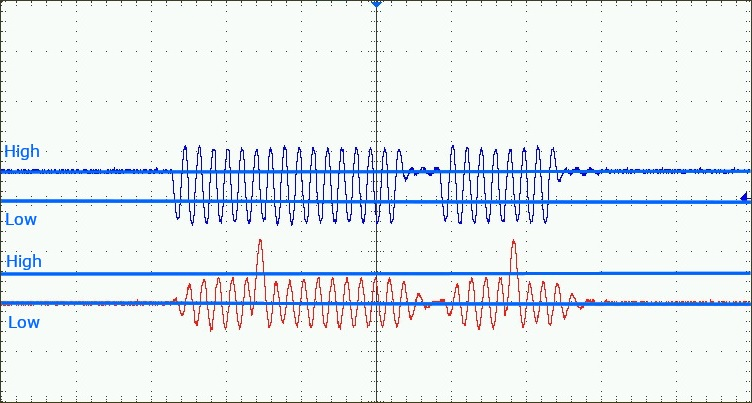
\includegraphics[width=0.75 \textwidth]{F0010TEK.jpg}
	\caption{Serial Data and Clock Signal to LED Driver Circuit}
	\label{fig:serdatclkLED}
\end{figure}
\noindent Figure \ref{fig:serdatclkLED} shows the signal being sent from the \ac{uc} to the \ac{led} driver circuit used. This signal is in the form of three consecutive bytes in serial. A signal that is not shown is the enable pin that is pulled low while the data is being sent, and otherwise is pulled high. The top signal (dark blue) is the clock used for the \ac{spi} transmission, the lower signal (red) is the data being sent in serial. As the data value is sampled at every rising edge of the clock pulse the data can be seen as $(0000\ 0100\ 0000\ 0000\ 0000\ 1000)_2$. This translates to the column data being $(0000\ 0000\ 0000\ 0100)_2$ and the row data being $(0000\ 1000)_2$ as the data is sent through as the lower column byte, the higher column byte, and the row byte. Thus, the signal being sent in this figure is lighting up the \ac{led} on the twelfth column and last row. The oscillations and overshoot seen in both signals can be attributed to the very high toggling speed of the \ac{spi} clock. This, however, does not cause an issue with the Shift Registers as the sampled voltages are below or above the minimum high and maximum low voltages \cite{595}.
\newpage
\subsection{LED Driver Output}
\begin{figure}[h!]
	\centering
	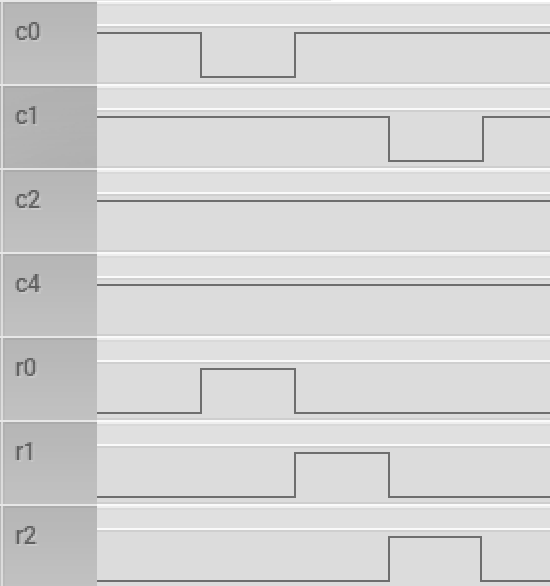
\includegraphics[width=0.4 \textwidth]{led_parallel.PNG}
	\caption{Output Signals from LED Driver}
	\label{fig:ledDriveOut}
\end{figure}
\noindent Figure \ref{fig:ledDriveOut} shows parts of the output from the \ac{led} matrix driver. Columns zero through four, and rows zero through two are shown. Two \acap{led} are selected, powered on, in this figure. These \acap{led} are at the first row and column (c0;r0), and the second column and third row (c1;r2). This figure not only shows the selected \acap{led} but also that the delay between each following state is negligible.
\section{Button Matrix}
\subsection{Serial Signal to Button Driver}
\begin{figure}[h!]
	\centering
	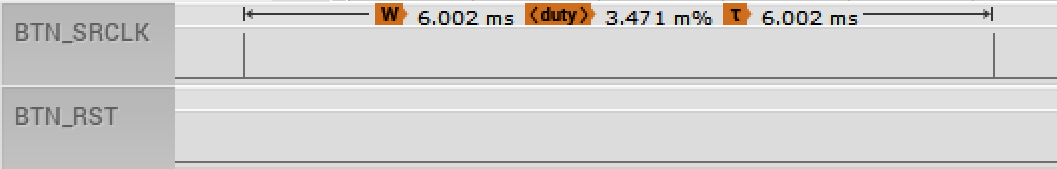
\includegraphics[width=0.6 \textwidth]{btn_serial.PNG}
	\caption{Serial Data to Button Matrix Driver}
	\label{fig:serdataBTN}
\end{figure}
\noindent The driver for the button matrix simply requires a clock signal to increment, and a reset signal in the case it is needed. The signal used to increment the output state does not have to be at a near 50\% duty cycle, a short pulse is sufficient. Figure \ref{fig:serdataBTN} shows the time between each column incrementation for the button matrix, with no reset occurring. The time between one incrementation and the next can be measured to be 6.002ms with a duty cycle of $3.471 (10)^{-3}$\%, which works out to 208.33ns for the incrementation pulse. 
\newpage
\subsection{Button Driver Output}
\begin{figure}[h!]
	\centering
	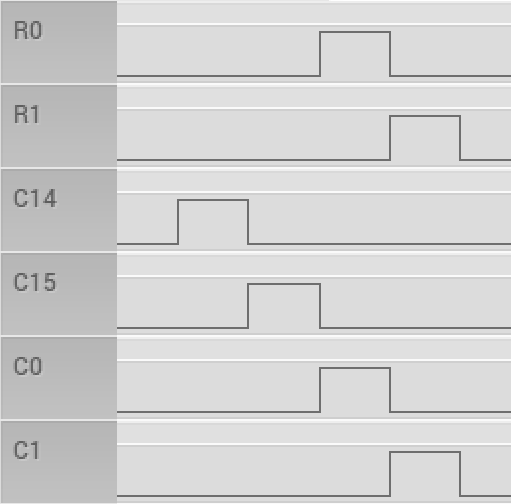
\includegraphics[width=0.4 \textwidth]{btn_parallel.PNG}
	\caption{Button Driver Output and Selected Rows}
	\label{fig:btnOutSelected}
\end{figure}
\noindent As designed for in hardware, the selected column is incremented over and wraps around, once it reaches the final column, to the first column. Figure \ref{fig:btnOutSelected} shows not only the columns incrementing and wrapping correctly but also two rows with some depressed buttons. When a button is selected a high voltage can be measured on the appropriate row pins. A sample of these row pins is taken every time the columns are incremented. The selected buttons in this figure are therefore at the first row and column (R0;C0), as well as the second row and column (R1;C1). This can be shown as when column zero is selected (high) row zero gets pulled high, indicating a selected button. This technique is replicated for all time states (columns).
\subsection{Timing Between Signals}
\begin{figure}[h!]
	\centering
	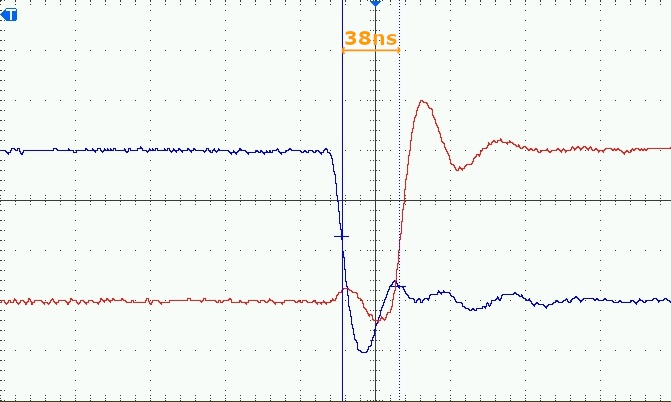
\includegraphics[width=0.6 \textwidth]{F0004TEK.JPG}
	\caption{Timing for Button Driver between Column 15 and 0}
	\label{fig:timingBtns}
\end{figure}
\noindent As the longest delay between button states would be observed between column 15 and column 0 when incrementing, due to requiring the \acap{ic} to reset, the delay was measured in Figure \ref{fig:timingBtns}. The time between column 15 going low and column 0 going high is measured to be approximately 38ns. This leads to this delay being considered negligible.
\section{LCD}
\subsection{Initialization Sequence}
\begin{figure}[h!]
	\centering
	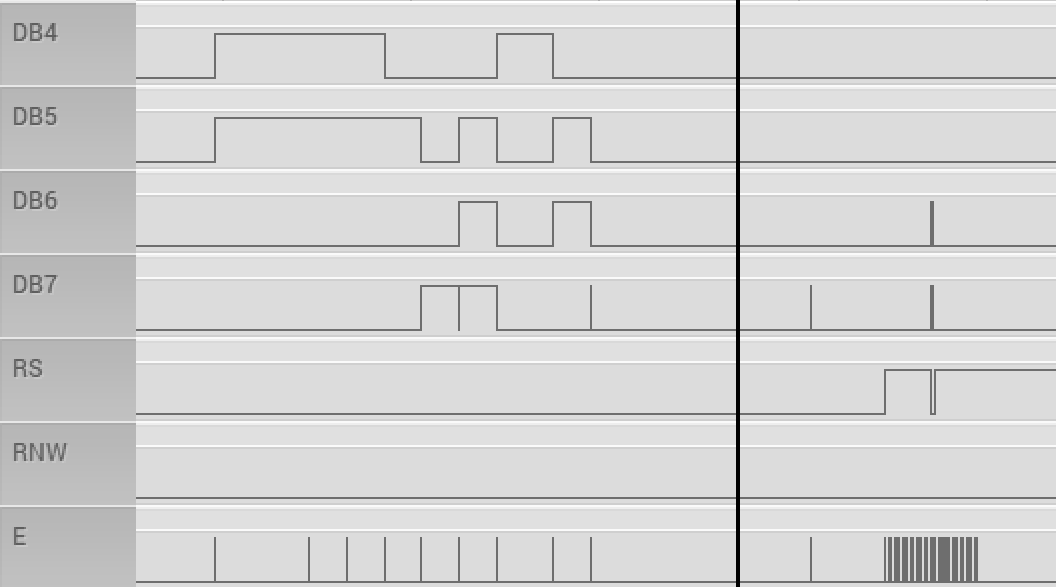
\includegraphics[width=0.7 \textwidth]{LCD_Init.PNG}
	\caption{Initialization Sequence of the LCD }
	\label{fig:lcdInit}
\end{figure}
\noindent During the first milliseconds of the main software loop running, the \ac{lcd} panel is initialized. The data being sent to the \ac{lcd} and time between commands can be found in Table \ref{tab:LCDfsm} \cite{lcd}. This data can be visualised in Figure \ref{fig:lcdInit}. The data nibbles that are transferred are visible as a parallel signal with the respective control signals below. The spikes shown in the row labeled \textit{E} represent the data being sent according to how the controller on the \ac{lcd} expects the data signals. The first data point to be sent over can be seen to be $(0011)_2 = (3)_{10}$ with RS = 0, this matches the required data as seen in the aforementioned table. The black vertical bar indicates a lapse in time as there is a large gap in this location due to the 100ms delay. The right-most data being sent is the initial display data, this is covered in more detail in the next section.
\subsection{Screen Update}
\begin{figure}[h!]
	\centering
	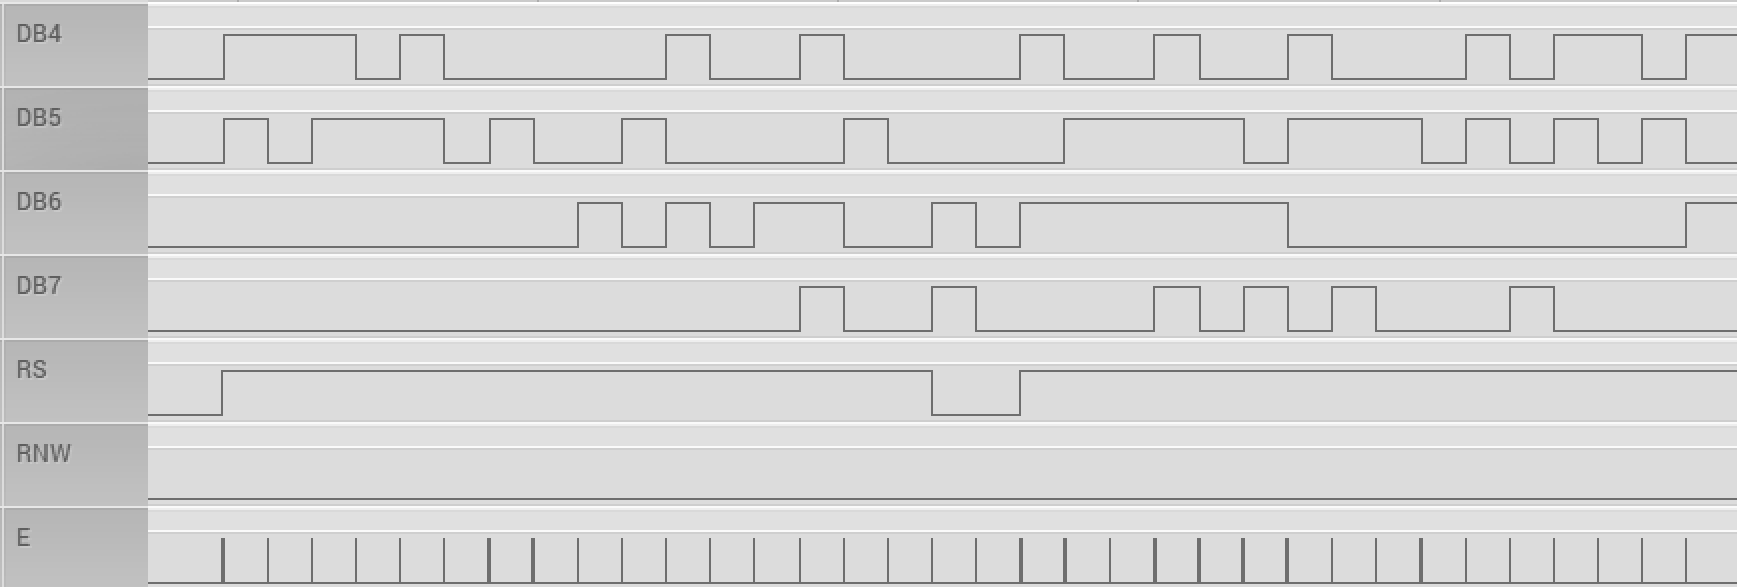
\includegraphics[width=0.8 \textwidth]{LCD_Data.PNG}
	\caption{Data being sent to the LCD}
	\label{fig:lcdDataExpl}
\end{figure}
\noindent Once the display has been initialized data can be sent from the \ac{uc}. This data is reconstructed on the \ac{lcd} and displayed \cite{lcd}. The signal shown in Figure \ref{fig:lcdDataExpl} displays the message "120 BPM Vol: 81\%". Each byte of \ac{ascii} data is split over two E toggles, better put, over two nibbles. Near the middle of the figure, RS goes low for the memory location change command. 
\section{UART Communication}
\subsection{Receiving Data}
\begin{figure}[h!]
	\centering
	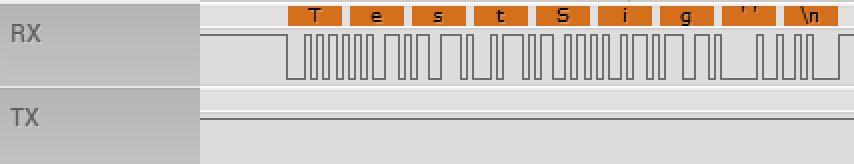
\includegraphics[width=0.6 \textwidth]{uart.PNG}
	\caption{Receiving UART Data from the FT230XS \cite{ft230x}}
	\label{fig:uartRX}
\end{figure}
\noindent As the \ac{uart} transceiver is unused no transmitted signal can be measured, however, data can still be sent from a PC to the \ac{uc}. Figure \ref{fig:uartRX} shows decoded text data coming into the \ac{uc} from a PC. This message was sent at 9600 \ac{baud} with 8-bit data, one stop bit, and no parity bits. 
\section{Audio Data}
\subsection{\ac{i2s} Data}
\begin{figure}[h!]
	\centering
	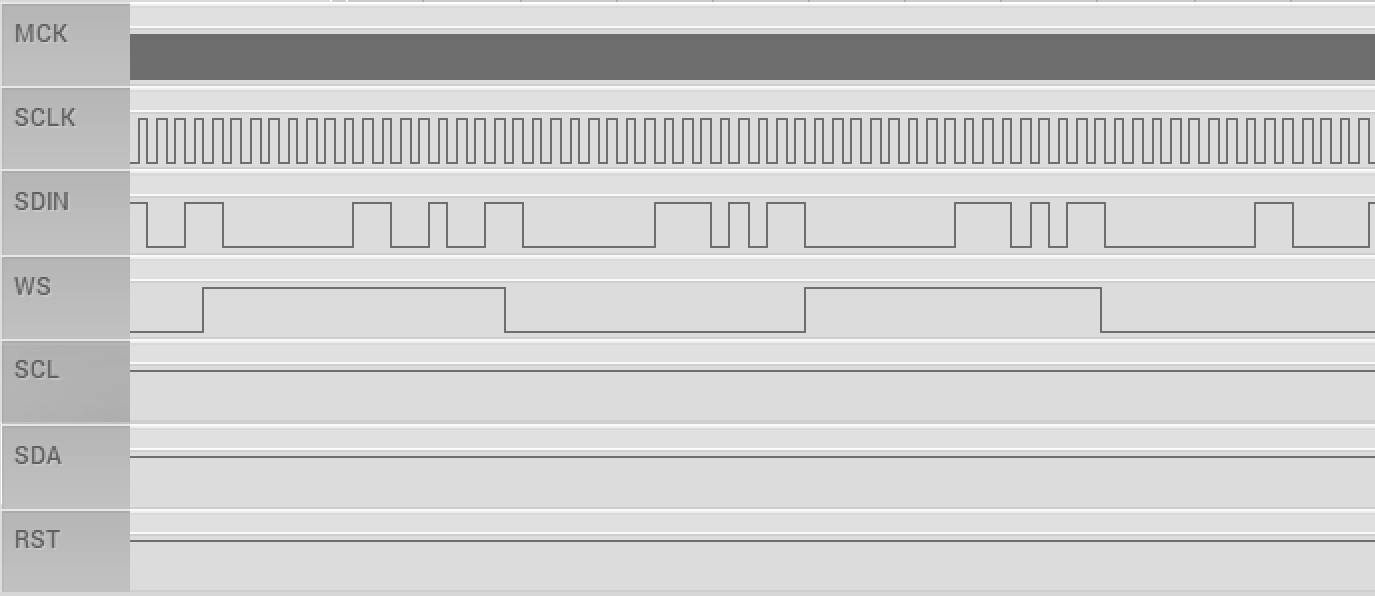
\includegraphics[width=0.8 \textwidth]{i2s.PNG}
	\caption{\ac{i2s} Data being sent to the \ac{dac}}
	\label{fig:i2sDac}
\end{figure}
\noindent Transmitting the \ac{pcm} data from the \ac{uc} to the \ac{dac} is handled by \ac{i2s} \cite{dac, f411brd}. The signals shown in Figure \ref{fig:i2sDac} represent the clocks, data and select used to transmit data over this standard. MCLK represents the Master Clock and is only used to synchronise internal \ac{dac}s and \ac{adc}s, not for the data transfer itself, thus the much higher frequency. SCLK is the serial clock used to sample the data on SDIN line. WS, or word select, is used to indicate which channel is being transferred, low is Left Channel, and high is Right \cite{i2s}. The other pins are used in the \ac{i2c} standard, but as no settings on the \ac{dac} are being changed these all remain low in the figure. It should be noted that there are sixteen SCLK cycles per channel, as each \ac{pcm} sample is 16-bit.
\newpage
\subsection{Audio Out}
\begin{figure}[h!]
	\centering
	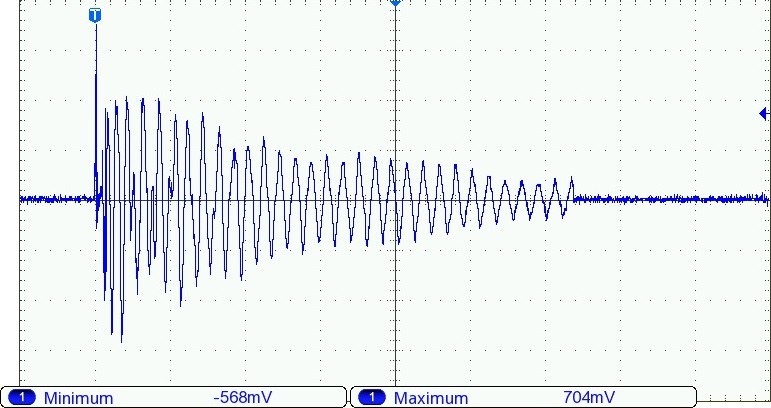
\includegraphics[width=0.6 \textwidth]{F0009TEK.jpg}
	\caption{The Audio Signal Produced by the \ac{dac}}
	\label{fig:dacOut}
\end{figure}
\noindent Figures \ref{fig:dacOut} and \ref{fig:audioFile} show the same audio file as generated by the \ac{dac} and shown on a PC respectively. The majority of the signal can be observed to be nearly the same, as is expected. The most notable differences, apart from the dead space before and after the audio in Figure \ref{fig:dacOut}, are the sound being cut off at the end, and a loud spike at the start of the audio. The audio stopping 'early' can be attributed to the \ac{dma} buffer for the audio never getting the last, up to, 1024 samples, thus ending the sound as it does. A further explanation of this can be found in Section \ref{sec:fillingAud}. The other issue, the spike at the start of the audio, could possibly be attributed to the file header also being read as audio data. This header is short enough that the time it takes to play back is inaudible.
\begin{figure}[h!]
	\centering
	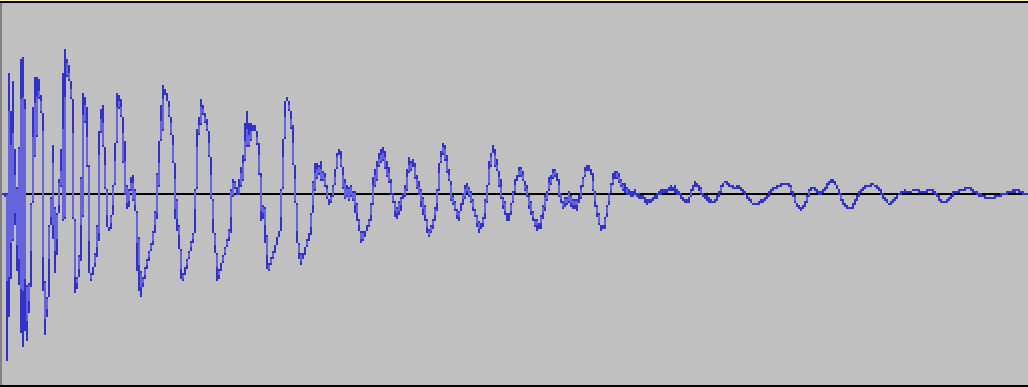
\includegraphics[width=0.6 \textwidth]{audFile.PNG}
	\caption{The Audio Signal Visualized on a PC}
	\label{fig:audioFile}
\end{figure}
\newpage
\section{Complete Drum Machine} \label{sec:fullMachine}
Figure \ref{fig:fullSysWorking} shows the Completed Drum Machine running with several beats selected. More detailed images can be found in Appendix \ref{sec:photosSys}.
\begin{figure}[h!]
	\centering
	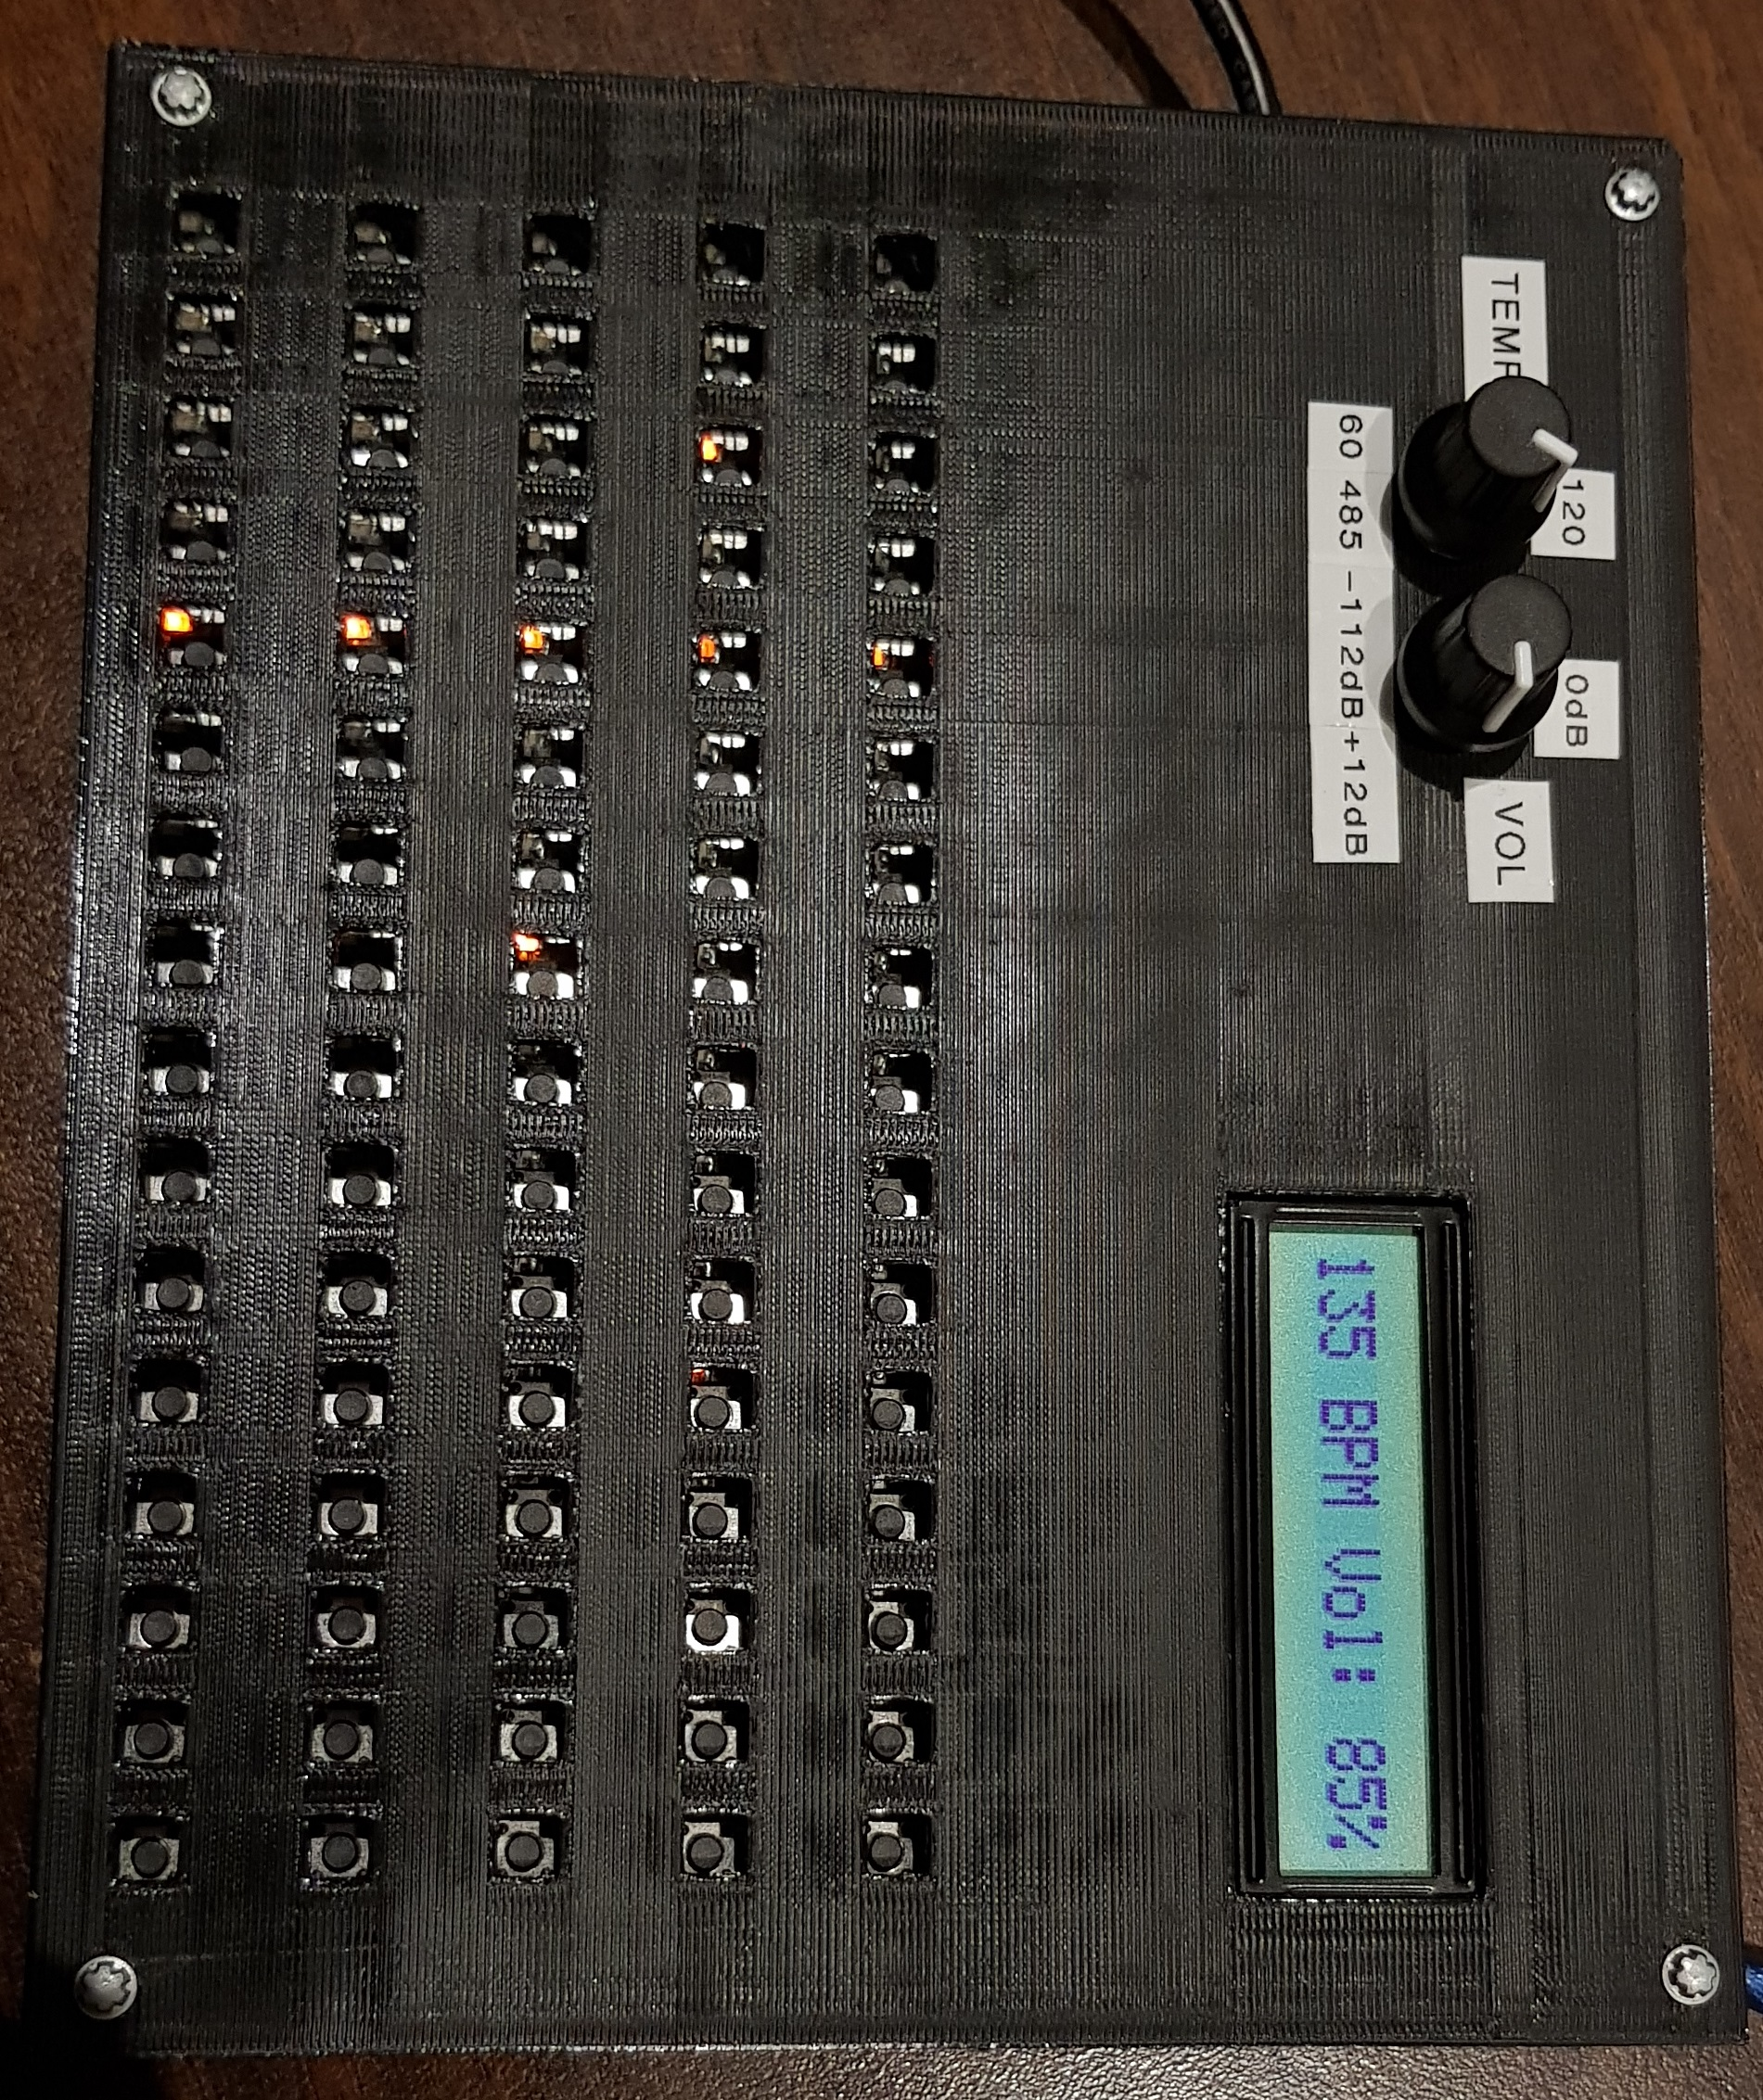
\includegraphics[width=0.9 \textwidth, angle=180]{angleFull.jpg}
	\caption{Completed Drum Machine Running}
	\label{fig:fullSysWorking}
\end{figure}\\
Button extenders and \ac{led} diffusers are not present in the figure above. This will be implemented by making these out of hot glue as this is a rigid material that diffuses light well.

%----------------------------------------------------------------------------------------
%	SECTION 6
%----------------------------------------------------------------------------------------
\chapter{Conclusions and Recommendations}
\section{Outcomes}
The Drum Machine functions correctly and satisfies all the requirements mentioned in Section \ref{sec:specs}. The system successfully displays the current tempo and volume to the user. These values can be changed within reasonable margins by making use of two potentiometers as voltage dividers. The matrix of \acap{led} and buttons is driven by only ten pins, greatly reduced from driving each row and column individually. The refresh rate of the \acap{led} and buttons is fast enough to not be noticeable to the user. A top panel was designed and 3D printed to fit the \ac{pcb} with stand-offs. \ac{uart} communication is possible. The tempo timing is accurate, allowing for correct scheduling. Playback of audio is clear and is scheduled as expected. The \ac{usb} interface successfully transfers wave files to the \ac{uc} for playback. Considering all this, the project is seen as a success.
\section{Shortcomings}
Though the Drum Machine does function some of the features have shortcomings. The rate at which the \ac{lcd} data is updated is directly linked to the tempo of the system. This causes reduced responsiveness when the tempo is low. The maximum tempo is currently determined by an in-line resistor, this causes the limit to be approximate, a limit in software would prove more accurate. The current \ac{led} driver circuit design can be improved by driving up to sixteen \acap{led} simultaneously rather than the current five. The method to achieve this is mentioned in Section \ref{sec:LEDDrvr}. The current software implementation reflects how the hardware should be set up, this is also incorrect here, limiting the maximal current to the \acap{led}. Pressing the buttons under the 3D printed panels is currently difficult as there are no button extenders and light diffusers. This can be implemented by using hot glue, this is further explained in Section \ref{sec:fullMachine}. Perhaps the largest shortcoming is the limit placed on the size of the audio files. This could possibly have been reworked to be read dynamically, as explained in Section \ref{sec:readUSB}, allowing larger file sizes and more channels.
\newpage
\section{Possible Improvements}
Even though the Drum Machine functions well, there are several improvements that can be made to make this a better product. Some of the items mentioned would improve the way in which the user will interact with the device, others would simply add more features.\\
To achieve the former several items could be integrated. Connections could be broken out on a separate \ac{pcb} allowing the user to be able to plug in all necessary connections, such as the audio out, \ac{usb} \ac{otg} drive port, and power in, in one location. This can then be installed at the rear of the device. An alternative method to power the device can be implemented, this would allow for more than 500mA \cite{f411brd} to be used by the entire system. All of these additional features could be encased in a plexiglass, plastic, or metal enclosure that covers more than the top. The device could also be made thinner by incorporating all the hardware onto a single \ac{pcb} rather than using daughter boards, such as the \ac{uc} development board. \\
Further features that could be implemented on the drum machine could be some of the following. Flash memory could be incorporated allowing larger audio files to be saved on the device. Red-Green-Blue \acap{led} can be used to allow for differently coloured indicators. New software could connect via \ac{usb} on a PC and manage the audio samples on the drum machine. The device could also support \ac{midi} to connect to other \ac{midi} devices. The potentiometers could be replaced with a single rotary encoder and selection buttons to change settings on the device. A more detailed display could also be used to indicate more settings or information about the selected sounds. A final feature that could be implemented is an on-board synthesiser, removing the need for actual sound files as the system could generate them locally.

\newpage
%----------------------------------------------------------------------------------------
%	BIBLIOGRAPHY
%----------------------------------------------------------------------------------------
\addcontentsline{toc}{chapter}{Bibliography}
\printbibliography


%----------------------------------------------------------------------------------------

%----------------------------------------------------------------------------------------
%	APPENDIX
%----------------------------------------------------------------------------------------
\appendix
\chapter{Project Planning Schedule}

	\begin{longtable}[c]{|r|p{10cm}|}
		\hline
		\multicolumn{1}{|c|}{\textbf{Week Of}} & \multicolumn{1}{c|}{\textbf{Task Completed}} \\
		\hline
		04 Feb & Design Specifications \\
		\hline
		11 Feb & Design Specifications \\
		\hline
		18 Feb & Initial setup of ST board, CubeMX, GIT. \newline Edited Example Code. Made Arduino Test Code. \\
		\hline
		25 Feb & Layout and PCB design. \\
		\hline
		04 Mar & PCB Design and Manufacture. \\
		\hline
		11 Mar & LED Driver Coding with PCB Tidy Up \\
		\hline
		18 Mar & PCB Tidy Up and Assembly \\
		\hline
		25 Mar & PCB Design Updated and LED Driver Coding \\
		\hline
		01 Apr & Button, UART and ADC (Tempo) Coded  \\
		\hline
		08 Apr & LCD Coding and STM Audio Driver Added \\
		\hline
		15 Apr & Figuring out STM Audio Driver \\
		\hline
		22 Apr & File Reading from USB drive Coding \\
		\hline
		29 Apr & File Reading from USB drive Coding and \newline Playing with STM Audio Driver \\
		\hline
		06 May & Changed Audio Driver and Pre-Load Audio Files \\
		\hline
		13 May & Top Panel Manufacture and Report Writing \\
		\hline
		20 May & Report Writing \\
		\hline
		27 May & Report Writing \\
		\hline
		03 Jun & Hand In and Oral/Poster Preparations \\
		\hline
		10 Jun & Oral Presentation and Poster Hand In \\
		\hline
		\caption{Simplified Project Planning Schedule}
	\end{longtable}%

\chapter{ECSA Outcome Compliance}

\begin{longtable}[c]{|m{0.4\textwidth}|m{0.5\textwidth}|}
	\hline
	\multicolumn{1}{|c|}{\textbf{ECSA ELO}} & \multicolumn{1}{c|}{\textbf{Compliance}} \\
	\hline
	\endhead
	
	
	\textbf{ELO 1. Problem solving:} \newline Identify, formulate, analyse and solve complex engineering problems creatively and innovatively.& Several issues appear during the hardware design phase, each of which has multiple solutions proposed and explained. A notable example is that of driving large numbers of pins with as few pins as possible. This is identified in Section \ref{sec:pincountReduc}, various solutions are proposed and chosen from with thorough reasoning. \\
	\hline
	\textbf{ELO 2. Application of scientific and engineering knowledge:} \newline Apply knowledge of mathematics, natural sciences, engineering fundamentals and an engineering speciality to solve complex engineering problems. & Mathematical concepts are used throughout the software in terms of bit-wise logic and formulas to generate certain values (such as for BPM or timers). Some values, such as the time between each button matrix incrementation, are chosen as an educated guess. Including noise suppression capacitors throughout the system allows for more accurate signals. The problem of reducing pin count with ICs can be seen as an open ended problem. A basic understanding of music and the usage of the device are also required. \\
	\hline
	\textbf{ELO 3. Engineering Design:} \newline Perform creative, procedural and non‐procedural design and synthesis of components, systems, engineering works, products or processes.& The design of the most basic functionality of a drum machine was completed first. The time constraints do not allow for many additional features unless ahead of schedule. The research into what the product is was completed first. Design of hardware and software followed after that. The hardware design has several options for sub-systems to choose from, as discussed in Chapter 2. The device is legal to use and could benefit the client as it satisfies all their needs. \\
	\hline
	\textbf{ELO 4. Investigations, experiments and data analysis:} \newline Demonstrate competence to design and conduct investigations and experiments. & Measurements are made and reported on in this written work. The history and types of drum machines is explored in Chapter 2. During the development of the Audio Playback software registers of the micro-controller were manually read and compared to the appropriate manuals. Pins used to drive certain features had to be changed as the development board has on board pull down resistors, thus pulling the connected signal low. Logic analysers and oscilloscopes were used to analyse the signals produced by the various sub-circuits. Conclusions were taken from the results of each sub-circuit's behaviour as well as signals shown on the oscilloscope. \\
	\hline
	\textbf{ELO 5. Engineering methods, skills and tools, including Information Technology:} \newline Demonstrate competence to use appropriate engineering methods, skills and tools, including those based on information technology.& Software is written for the selected micro-controller in embedded-C. This code controls all the communications between sub-circuits and handles all of the data. Oscilloscopes, logic analysers, and the debugging tool in Atollic TrueStudio allowed for signal states at various points of the system to be tracked and compared to expected results. Design tools, Autodesk Fusion 360 and KiCAD, are used to create the 3D printed panel and PCB respectively.  \\
	\hline
	\textbf{ELO 6. Professional and technical communication:} \newline Demonstrate competence to communicate effectively, both orally and in writing, with engineering audiences and the community at large.& The written work is structured as to allow the reader to follow along the thought process of the design in all phases: going from what the device is, to designing it in hardware and software, to finally testing it. Figures and tables are placed throughout the document where they seem most appropriate and to aid in the explanation of certain concepts or designs. The written work was completed in \LaTeX and contains images from oscilloscopes and logic analysers. The oral presentation is presented in English with the use of a slideshow presentation and possibly the device itself. \\
	\hline
	\textbf{ELO 8. Individual work:} \newline Demonstrate competence to work effectively as an individual.& The entirety of this written work, design of hardware (including the PCB and 3D printed cover plate), design of software, measurement evaluation, oral presentation, and poster was all completed individually, with only minor guidance on possible changes given. \\
	\hline
	\textbf{ELO 9. Independent Learning Ability:} \newline Demonstrate competence to engage in independent learning through well-developed learning skills. & Knowledge on how to design the PCB and cover plate was gained externally from the University. Further design ideas, as referenced, for circuits were also obtained, modified and applied in the final system. The history, and thus type of drum machine to build, was explored and used to create a greater understanding of the final product. Several mistakes were made and were corrected or mentioned, as well as many alternate designs for certain circuits being measured. The assumption of the STM provided audio driver to work was challenged when it had to be replaced with that of a third-party which was adapted for this product. \\
	\hline
	
	\caption{ECSA ELO Compliance}
	\label{tab:ecsa}%
\end{longtable}%
	
\chapter{Circuit Diagram}
\begin{figure}[h!]
\begin{center}
	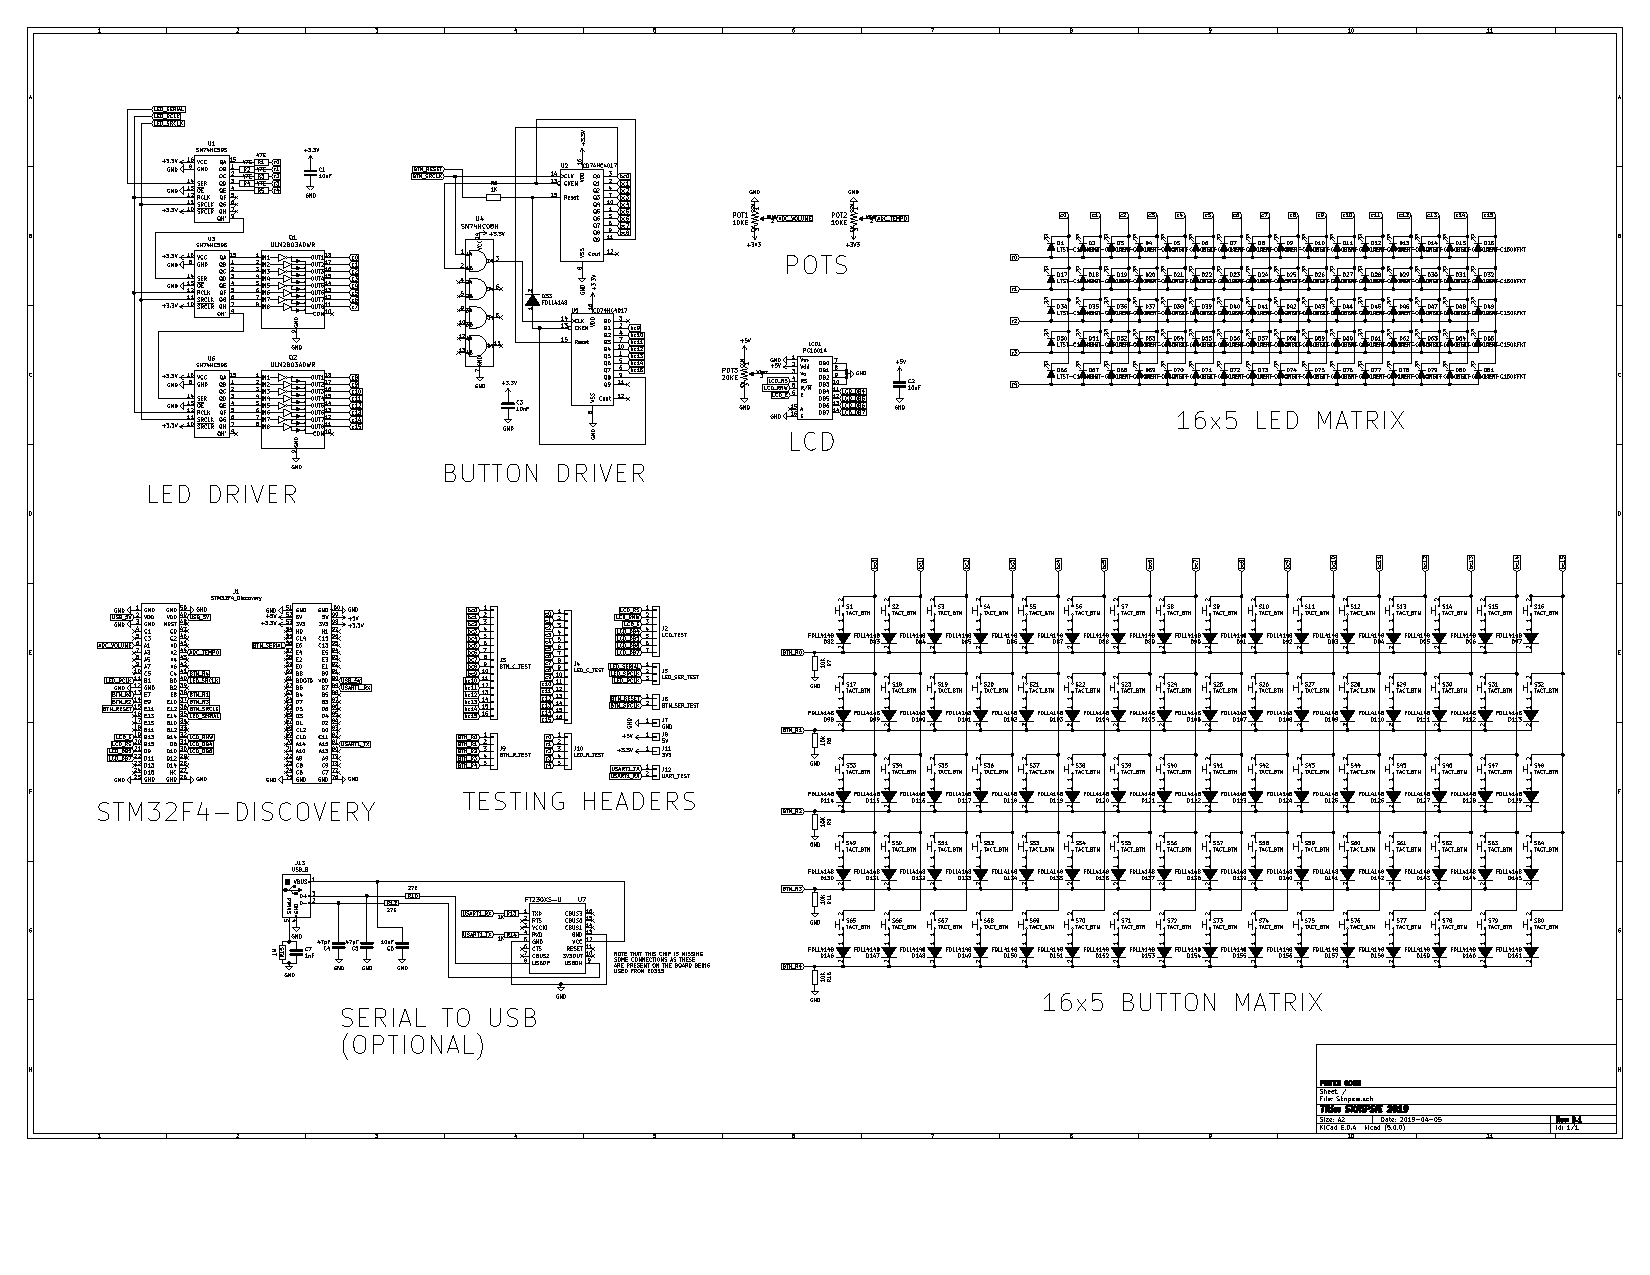
\includegraphics[width = \textwidth, angle=90, origin=c]{../Skripsie/Layout_05042019.pdf}
	\caption{The Final Revision (Rev. B.1) of the Circuit Diagram}
\end{center}
\end{figure}
\begin{figure}[h!]
	\begin{center}
		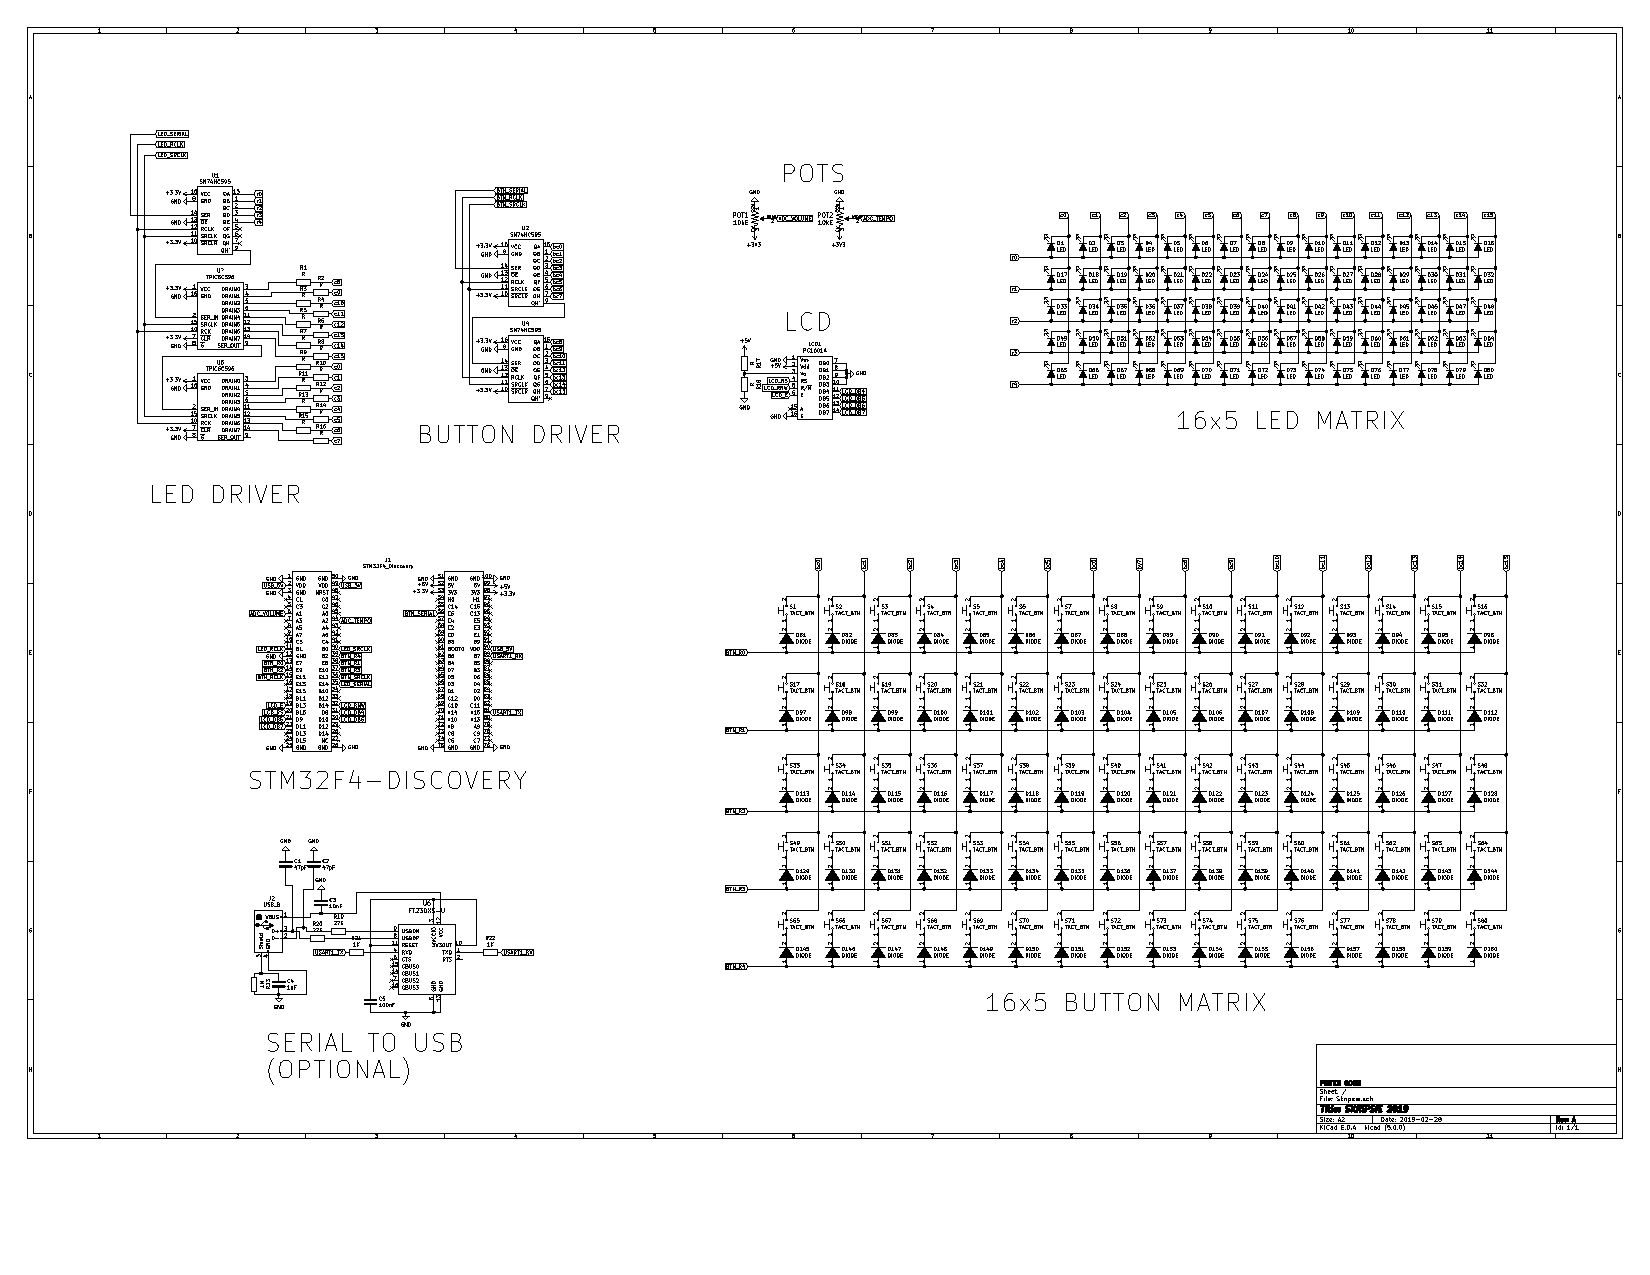
\includegraphics[width = 1.2 \textwidth, angle=90, origin=c]{../Skripsie/Layout_28022019.pdf}
		\caption{Revision A of the Circuit Design}
	\end{center}
\end{figure}

\chapter{PCB Design} \label{sec:PCB}
\begin{figure}[h!]
	\begin{center}
		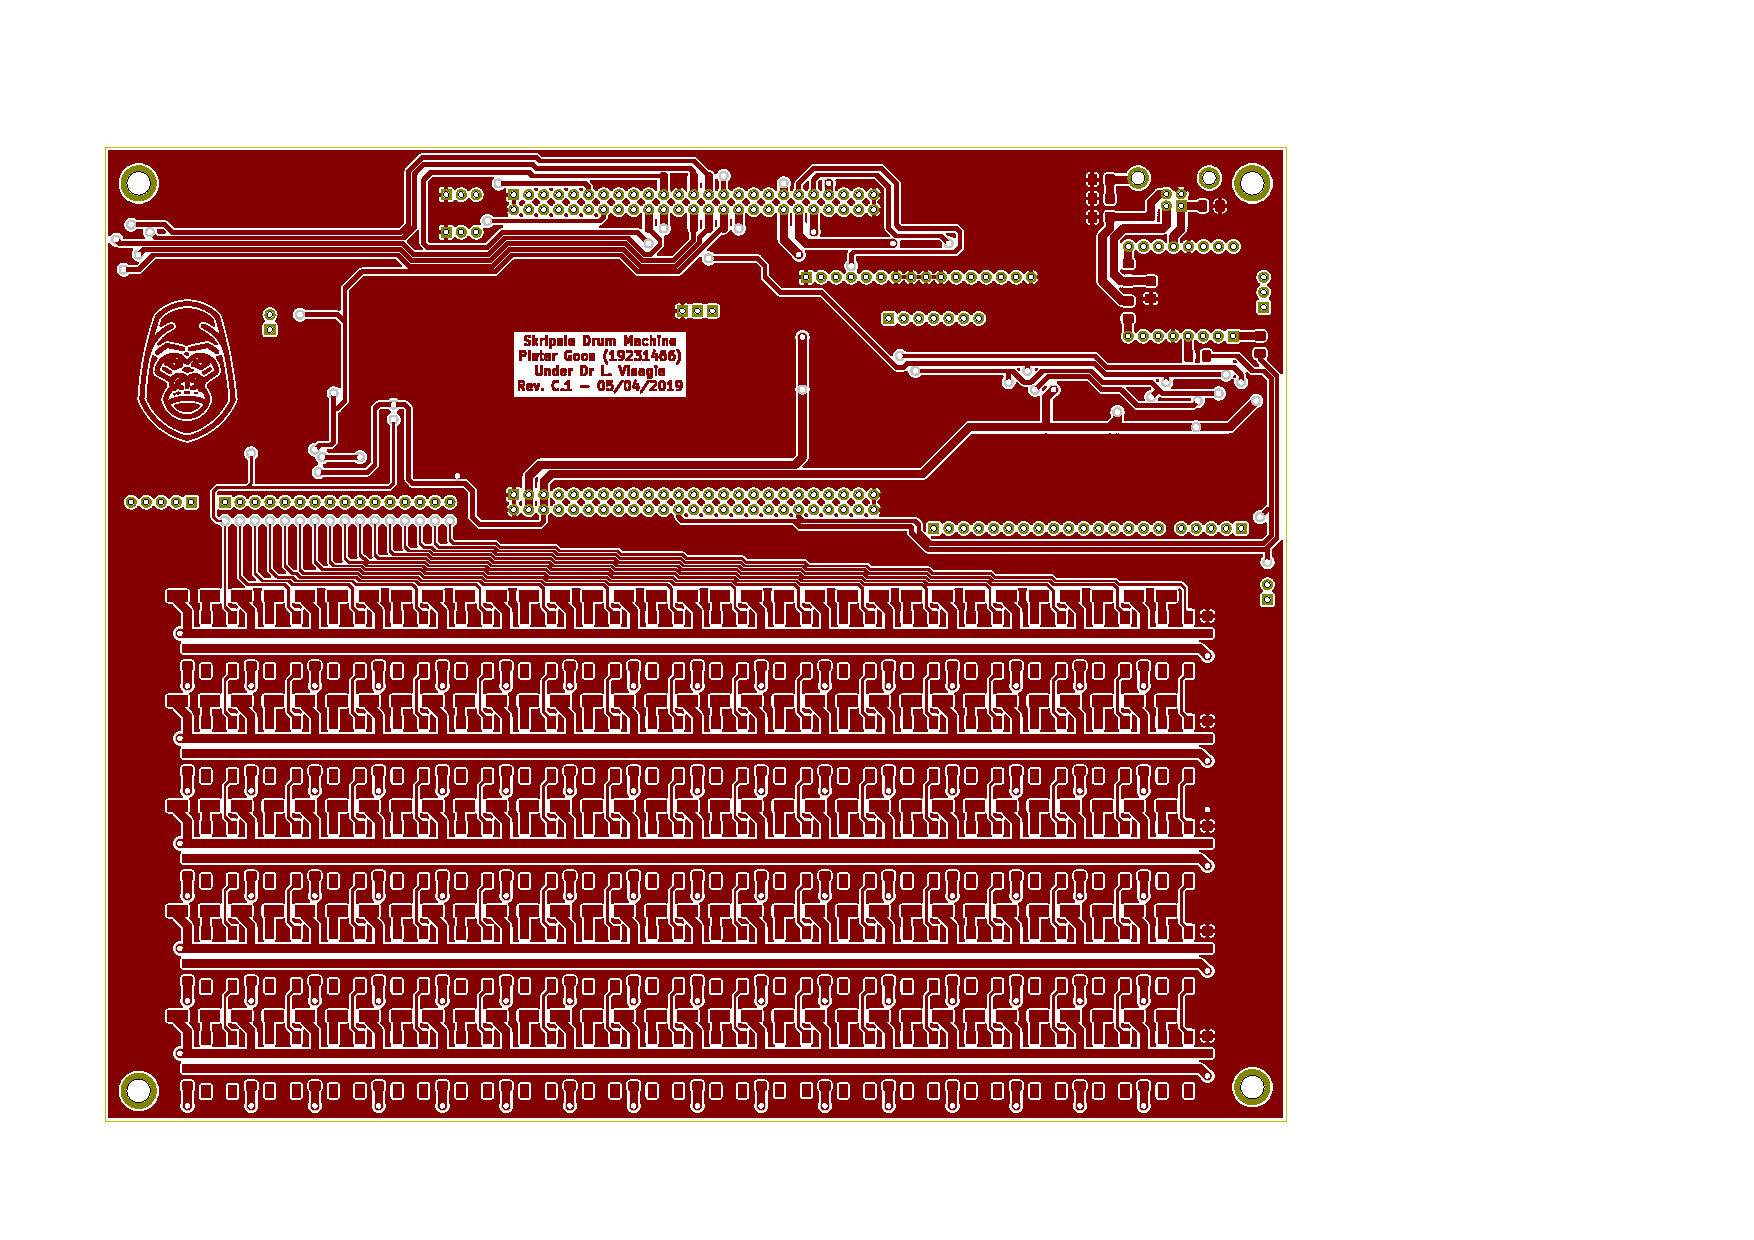
\includegraphics[width = \textwidth, trim={0.69in 0.78in 3.1in 0.95in}, clip]{../Skripsie/PCB_05042019.pdf}
		\caption{Front Copper Layer of Revision C.1 of the \ac{pcb}}
		\label{fig:frontpcb}
	\end{center}
\end{figure}
\begin{figure}[h!]
	\begin{center}
		\includegraphics[page=2, width = \textwidth, trim={0.69in 0.78in 3.1in 0.95in}, clip]{../Skripsie/PCB_05042019.pdf}
		\caption{Back Copper Layer of Revision C.1 of the \ac{pcb}}
		\label{fig:backpcb}
	\end{center}
\end{figure}
\noindent It is worth noting that this board (See Figures \ref{fig:frontpcb} and \ref{fig:backpcb}) shown is Revision C, however the board used to construct this project on is Revision B. The changes made between the two versions are simply forgotten and moved traces, and mounting holes have been added.\\
When looking at the reverse of the board (As in Figure \ref{fig:backpcb}) it is worth noting that the shown diagram is not mirrored. This implies that the diagram shown's top left corner matches that of the front copper layer, thus one would have to mirror this from left to right to see what you would see in reality.
\chapter{Images of Completed System} \label{sec:photosSys}
\begin{figure}[h!]
	\centering
	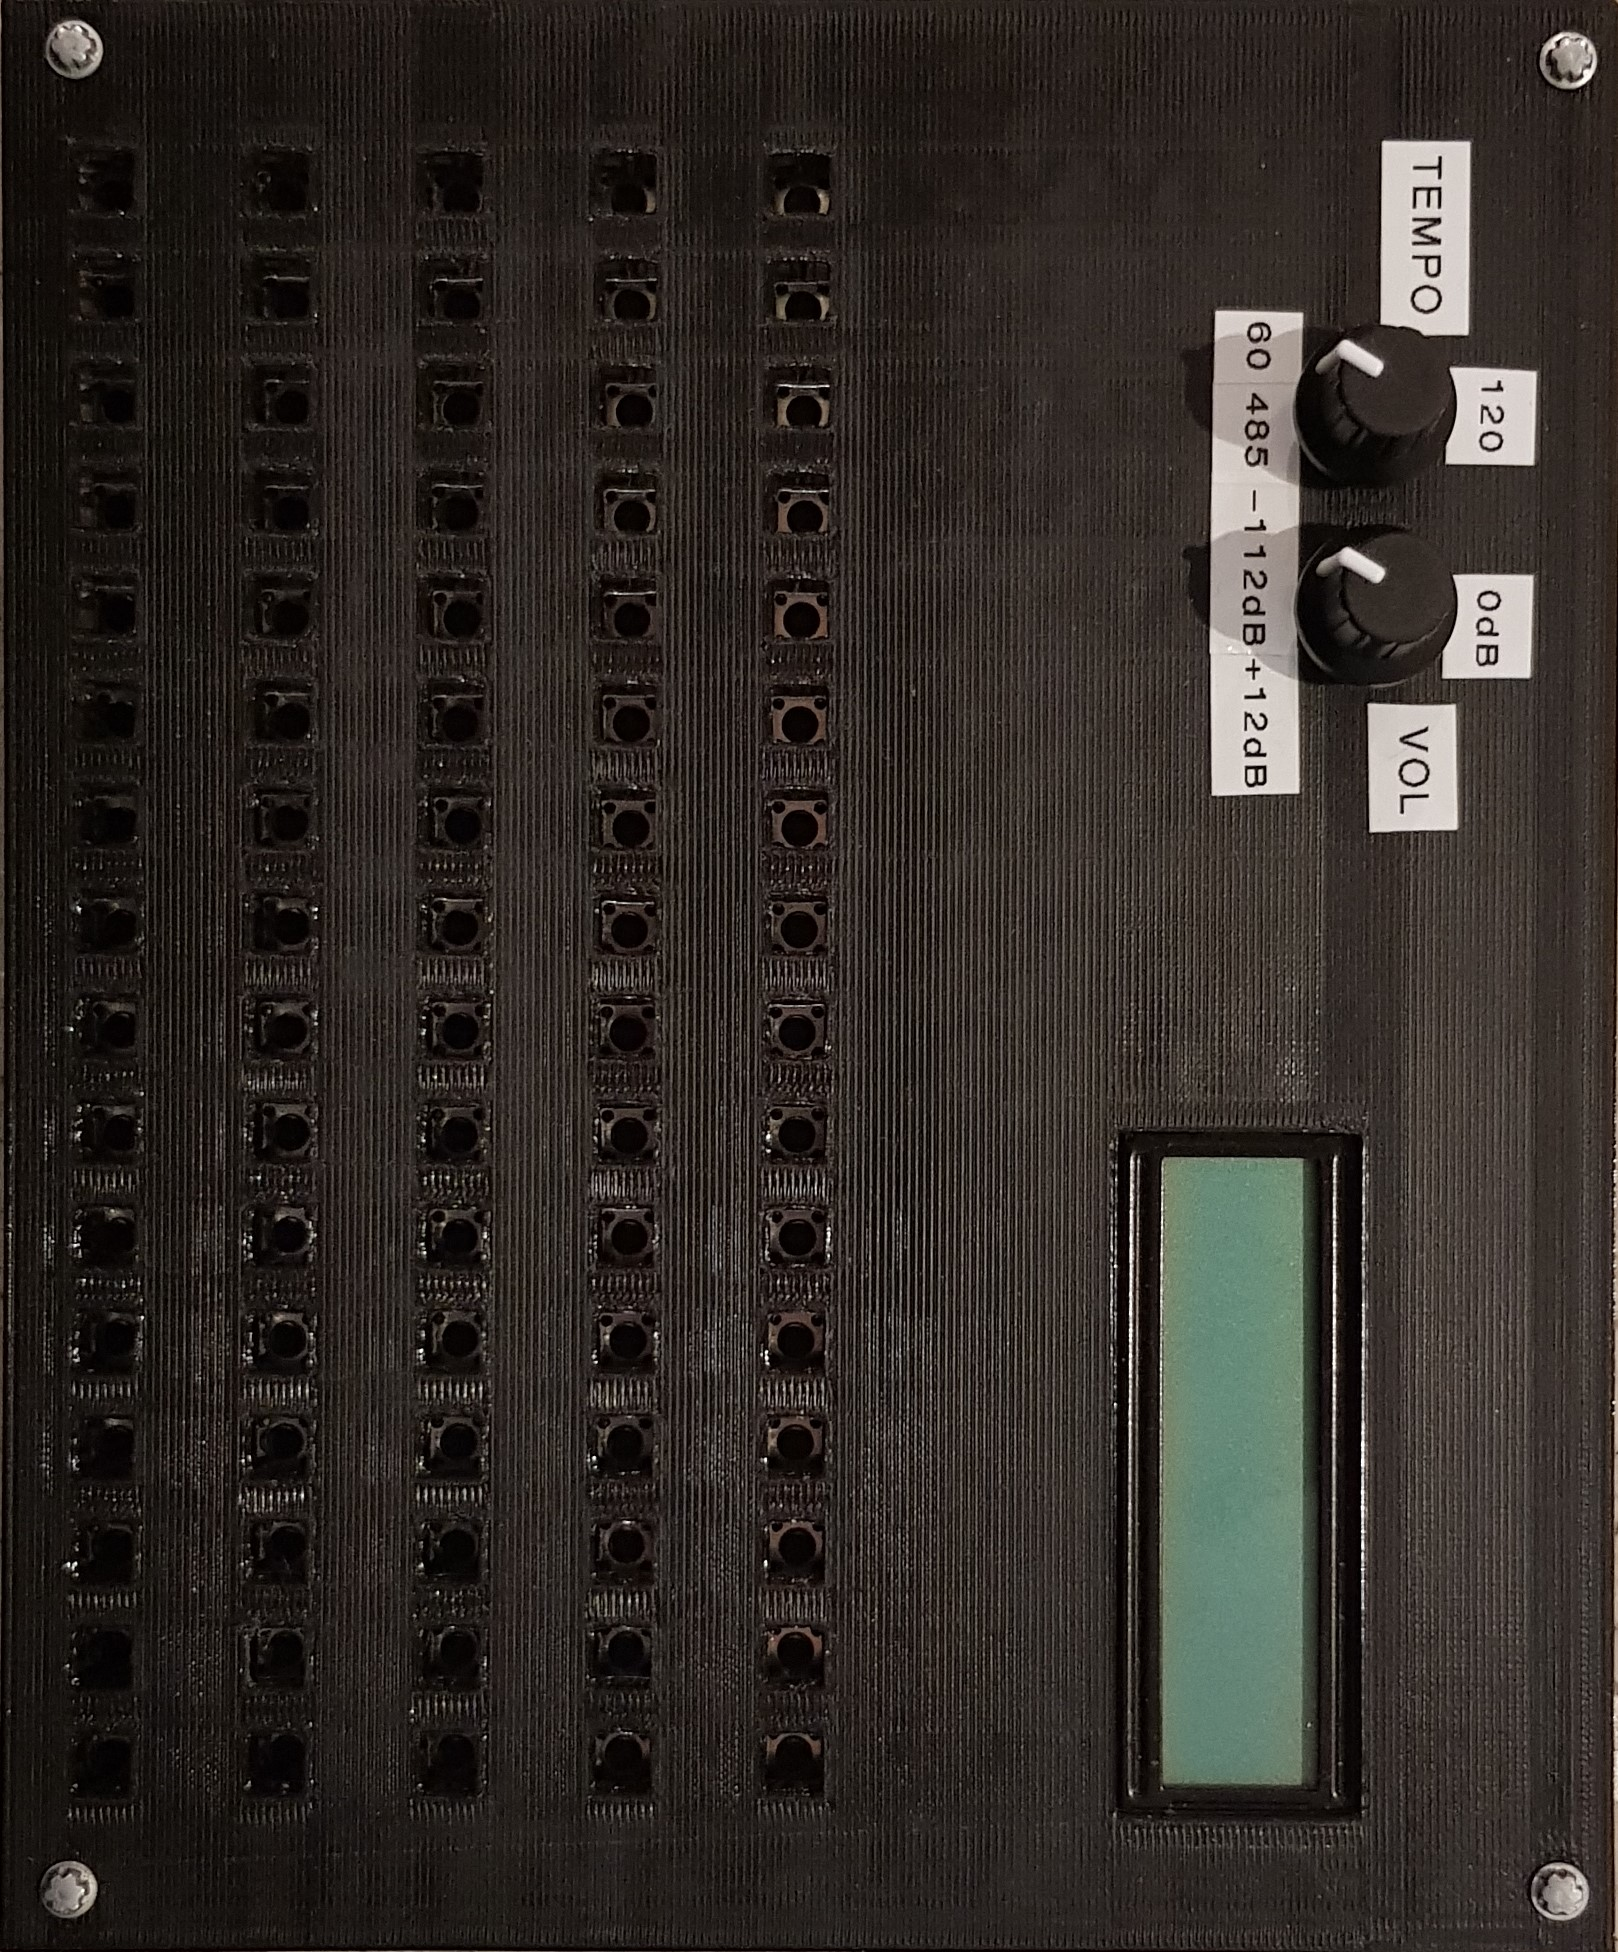
\includegraphics[width=0.8\textwidth, angle=90]{front_Panel.jpg}
	\caption{The top of the completed Drum Machine with 3D Printed Cover}
\end{figure}
\begin{figure}[h!]
	\centering
	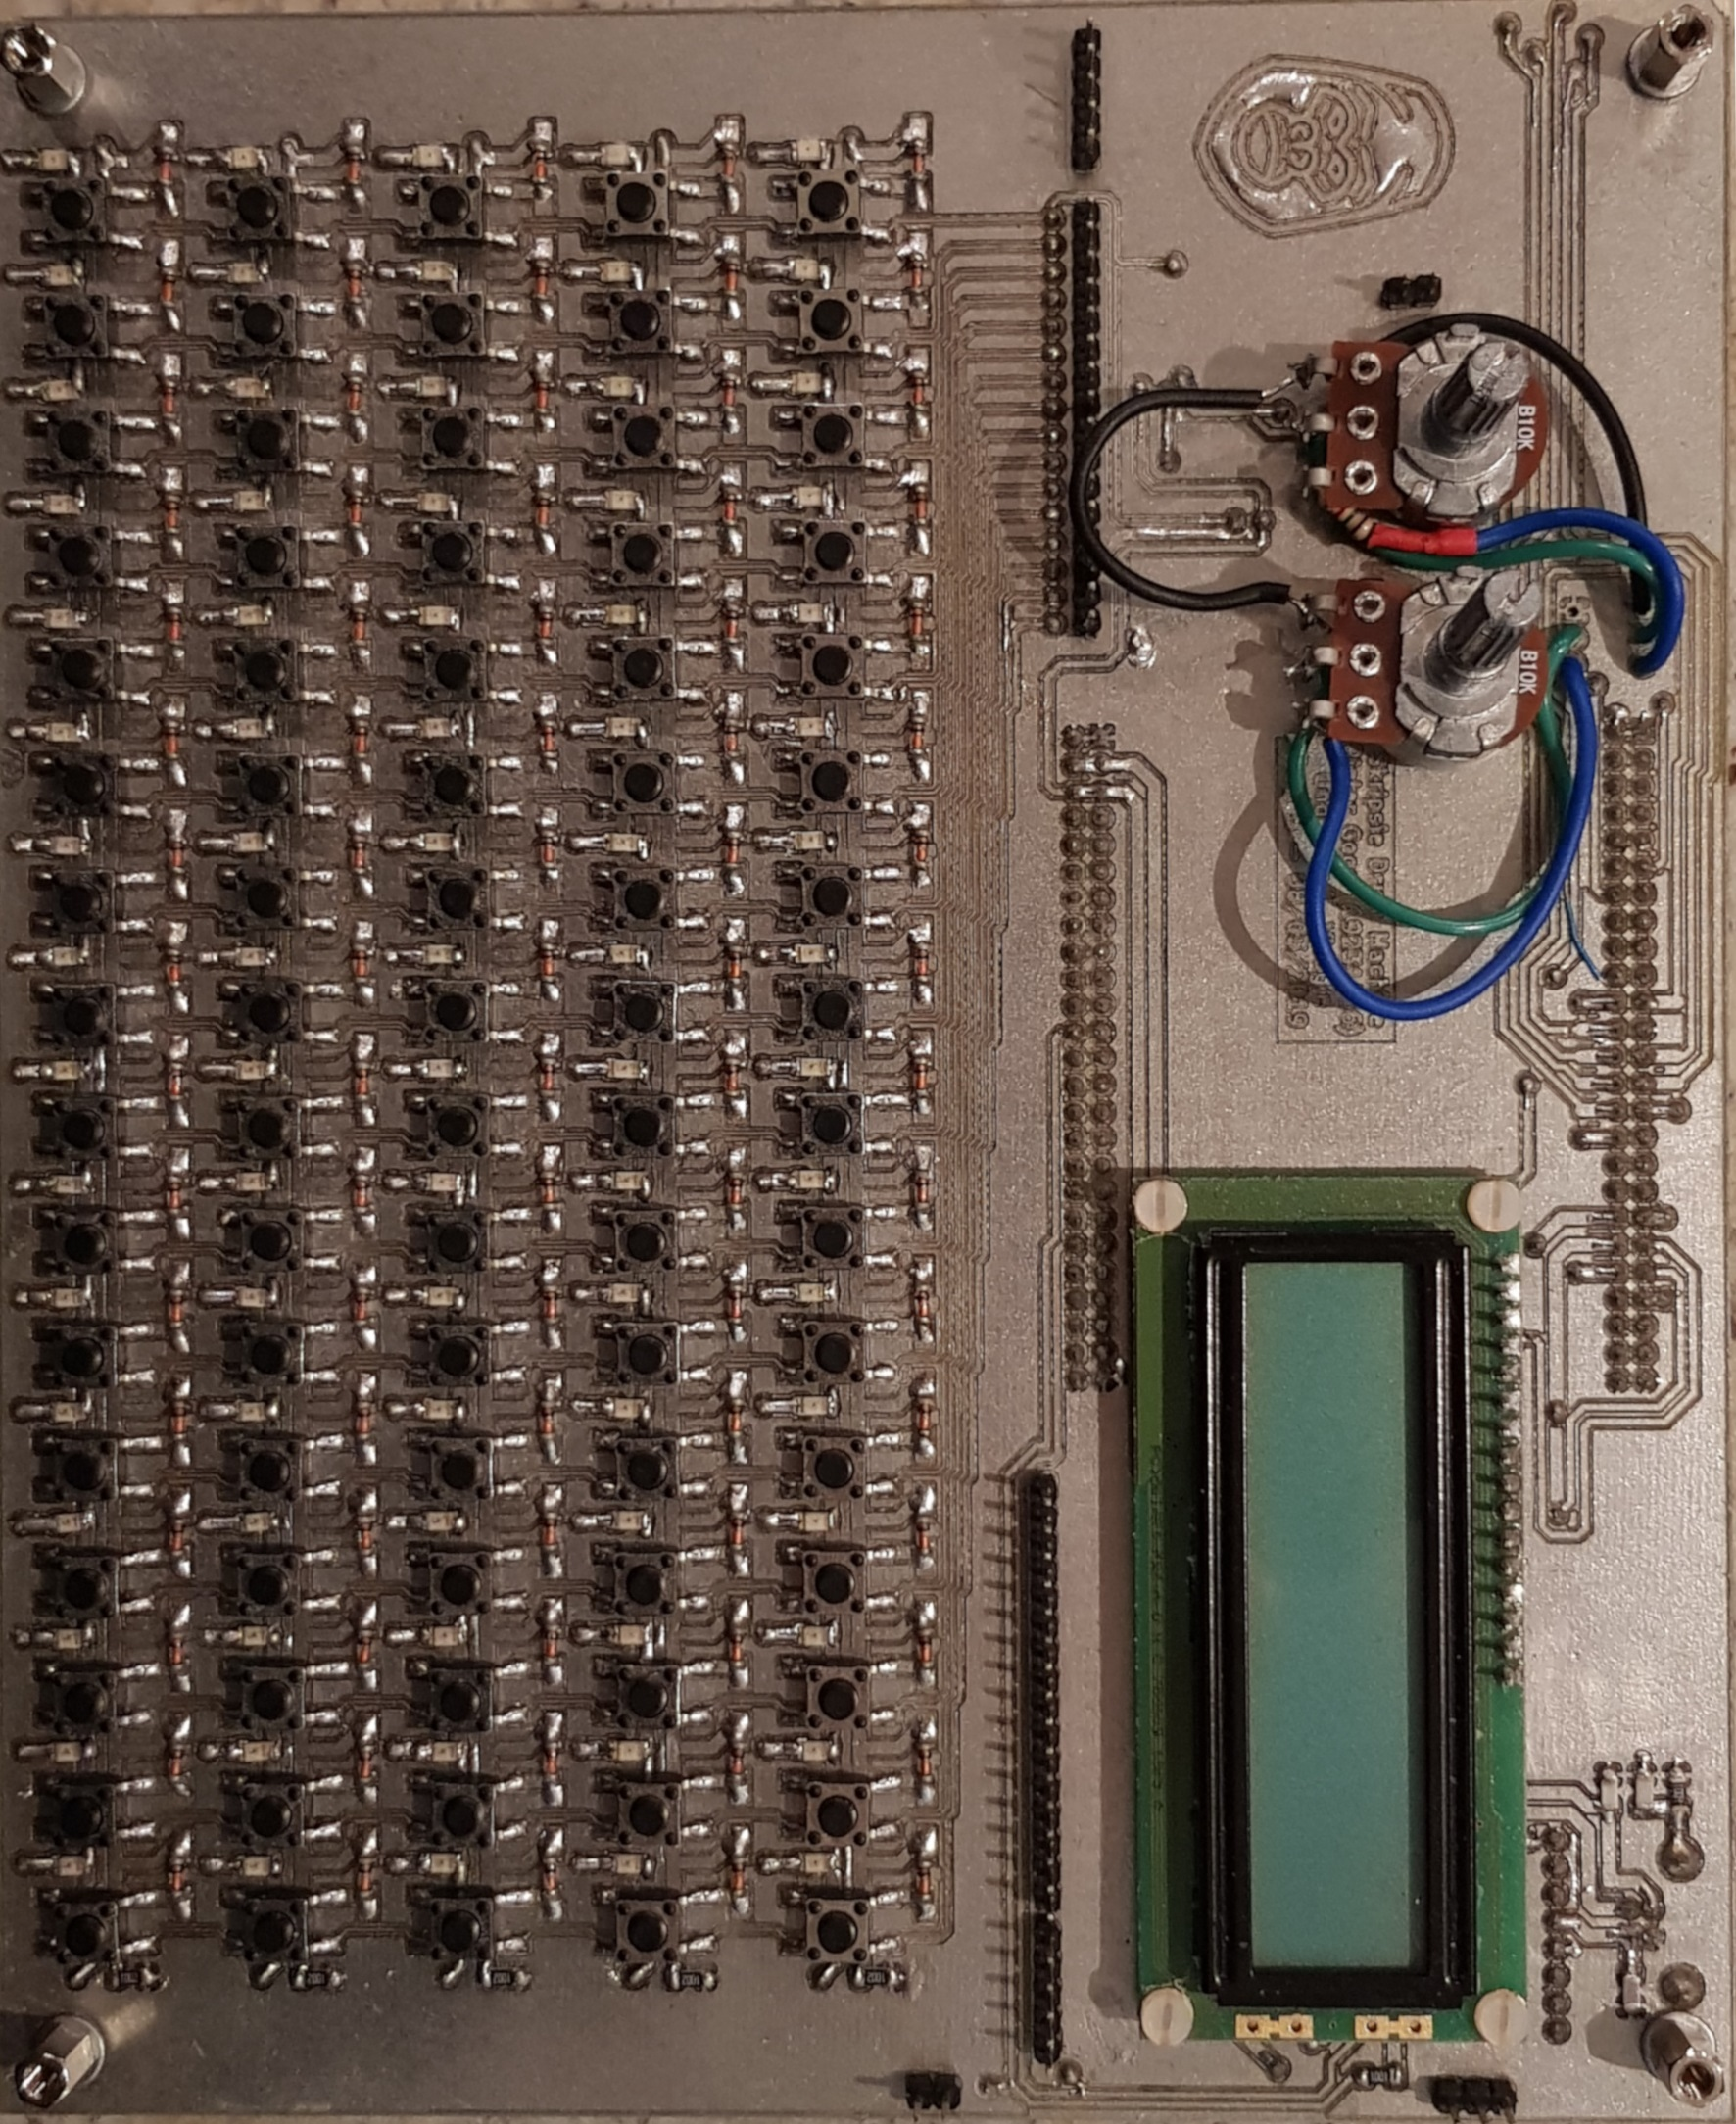
\includegraphics[height=0.5\textheight, angle=90]{front_noPanel.jpg}
	\caption{The top of the completed Drum Machine without the Cover}
\end{figure}
\begin{figure}[h!]
	\centering
	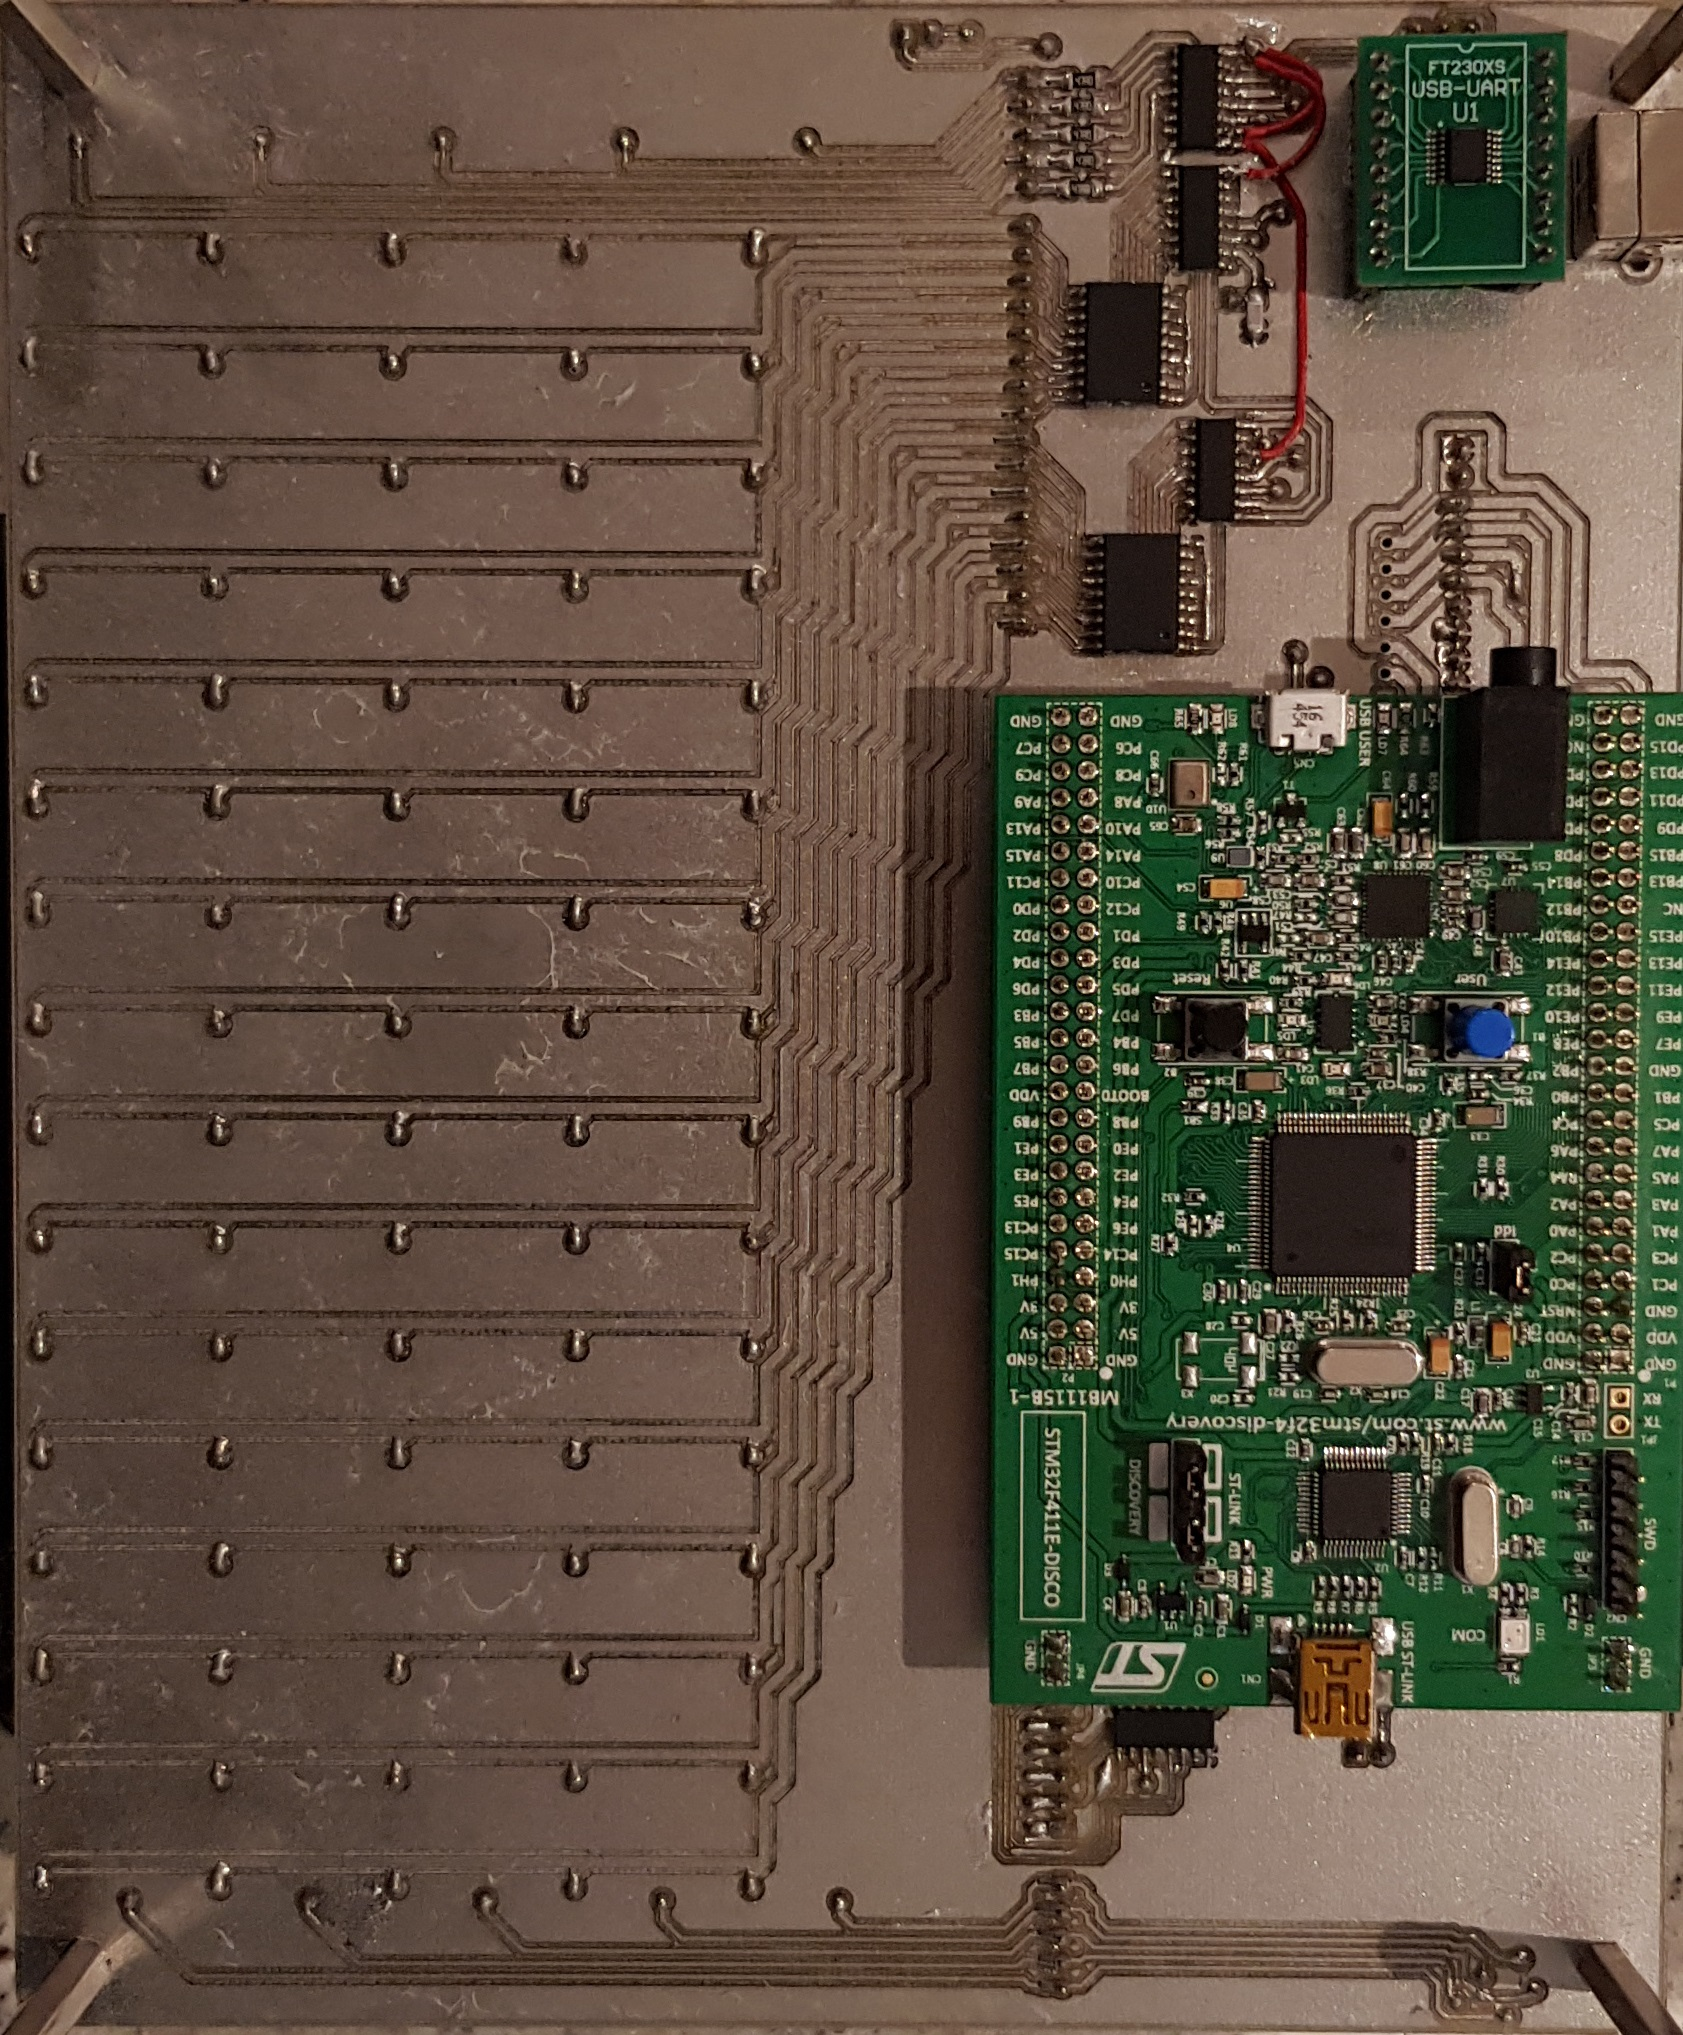
\includegraphics[height=0.5\textheight, angle=90]{back_UC.jpg}
	\caption{The botton of the completed Drum Machine}
\end{figure}
\chapter{Micro-Controller pinout}
\small
\begin{longtable}[c]{|r|l|l|r|r|}
		
		\hline
		\multicolumn{2}{|c|}{\textbf{Pin}} & \multicolumn{1}{c|}{\textbf{Type}} & \multicolumn{1}{c|}{\textbf{Signal}} & \multicolumn{1}{c|}{\textbf{Label}} \\
		\hline
		\endhead
		1     & PE2   & Input & \multicolumn{1}{l|}{GPIO\_Input} & \multicolumn{1}{l|}{DATA\_Ready [LSM303DLHC\_DRDY]} \\
		\hline
		2     & PE3   & Output & \multicolumn{1}{l|}{GPIO\_Output} & \multicolumn{1}{l|}{CS\_I2C/SPI [L3GD20\_CS\_I2C/SPI]} \\
		\hline
		3     & PE4   & I/O   & \multicolumn{1}{l|}{GPIO\_EXTI4} & \multicolumn{1}{l|}{INT1 [LSM303DLHC\_INT1]} \\
		\hline
		4     & PE5   & I/O   & \multicolumn{1}{l|}{GPIO\_EXTI5} & \multicolumn{1}{l|}{INT2 [LSM303DLHC\_INT2]} \\
		\hline
		5     & PE6   & I/O   &       &  \\
		\hline
		6     & VBAT  & Power &       &  \\
		\hline
		7     & PC13 & I/O   &       & \multicolumn{1}{l|}{ANTI\_TAMP} \\
		\hline
		8     & PC14 & I/O   & \multicolumn{1}{l|}{RCC\_OSC32\_IN} & \multicolumn{1}{l|}{PC14-OSC32\_IN} \\
		\hline
		9     & PC15 & I/O   & \multicolumn{1}{l|}{RCC\_OSC32\_OUT} & \multicolumn{1}{l|}{PC15-OSC32\_OUT} \\
		\hline
		10    & VSS   & Power &       &  \\
		\hline
		11    & VDD   & Power &       &  \\
		\hline
		12    & PH0& I/O   & \multicolumn{1}{l|}{RCC\_OSC\_IN} & \multicolumn{1}{l|}{PH0-OSC\_IN} \\
		\hline
		13    & PH1 & I/O   & \multicolumn{1}{l|}{RCC\_OSC\_OUT} & \multicolumn{1}{l|}{PH1-OSC\_OUT} \\
		\hline
		14    & NRST  & Reset &       &  \\
		\hline
		15    & PC0   & Output & \multicolumn{1}{l|}{GPIO\_Output} & \multicolumn{1}{l|}{OTG\_FS\_PowerSwitchOn} \\
		\hline
		16    & PC1   & I/O   &       &  \\
		\hline
		17    & PC2   & I/O   & \multicolumn{1}{l|}{I2S2\_ext\_SD} &  \\
		\hline
		18    & PC3   & I/O   & \multicolumn{1}{l|}{I2S2\_SD} & \multicolumn{1}{l|}{PDM\_OUT [MP45DT02\_DOUT]} \\
		\hline
		19    & VDD   & Power &       &  \\
		\hline
		20    & VSSA  & Power &       &  \\
		\hline
		21    & VREF+ & Power &       &  \\
		\hline
		22    & VDDA  & Power &       &  \\
		\hline
		23    & PA0 & I/O   & \multicolumn{1}{l|}{GPIO\_EXTI0} & \multicolumn{1}{l|}{WKUP} \\
		\hline
		24    & PA1   & I/O   & \multicolumn{1}{l|}{ADC1\_IN1} & \multicolumn{1}{l|}{ADC\_VOLUME} \\
		\hline
		25    & PA2   & I/O   & \multicolumn{1}{l|}{ADC1\_IN2} & \multicolumn{1}{l|}{ADC\_TEMPO} \\
		\hline
		26    & PA3   & I/O   &       &  \\
		\hline
		27    & VSS   & Power &       &  \\
		\hline
		28    & VDD   & Power &       &  \\
		\hline
		29    & PA4   & I/O   & \multicolumn{1}{l|}{I2S3\_WS} & \multicolumn{1}{l|}{I2S3\_WS [CS43L22\_LRCK]} \\
		\hline
		30    & PA5   & I/O   & \multicolumn{1}{l|}{SPI1\_SCK} & \multicolumn{1}{l|}{SPI1\_SCK [L3GD20\_SC/SPC]} \\
		\hline
		31    & PA6   & I/O   & \multicolumn{1}{l|}{SPI1\_MISO} & \multicolumn{1}{l|}{SPI1\_MISO [L3GD20\_AS0/SDO]} \\
		\hline
		32    & PA7   & I/O   & \multicolumn{1}{l|}{SPI1\_MOSI} & \multicolumn{1}{l|}{SPI1\_MOSI [L3GD20\_SDA/SDI/SDO]} \\
		\hline
		33    & PC4   & Input & \multicolumn{1}{l|}{GPIO\_Input} & \multicolumn{1}{l|}{BTN\_R4} \\
		\hline
		34    & PC5   & I/O   &       &  \\
		\hline
		35    & PB0   & I/O   & \multicolumn{1}{l|}{SPI5\_SCK} & \multicolumn{1}{l|}{LED\_SRCLK} \\
		\hline
		36    & PB1   & Output & \multicolumn{1}{l|}{GPIO\_Output} & \multicolumn{1}{l|}{LED\_RCLK} \\
		\hline
		37    & PB2   & I/O   &       &  \\
		\hline
		38    & PE7   & Input & \multicolumn{1}{l|}{GPIO\_Input} & \multicolumn{1}{l|}{BTN\_R0} \\
		\hline
		39    & PE8   & Input & \multicolumn{1}{l|}{GPIO\_Input} & \multicolumn{1}{l|}{BTN\_R1} \\
		\hline
		40    & PE9   & Input & \multicolumn{1}{l|}{GPIO\_Input} & \multicolumn{1}{l|}{BTN\_R2} \\
		\hline
		41    & PE10  & Input & \multicolumn{1}{l|}{GPIO\_Input} & \multicolumn{1}{l|}{BTN\_R3} \\
		\hline
		42    & PE11  & Output & \multicolumn{1}{l|}{GPIO\_Output} & \multicolumn{1}{l|}{BTN\_RESET} \\
		\hline
		43    & PE12  & Output & \multicolumn{1}{l|}{GPIO\_Output} & \multicolumn{1}{l|}{BTN\_CLK} \\
		\hline
		44    & PE13  & I/O   &       &  \\
		\hline
		45    & PE14  & I/O   & \multicolumn{1}{l|}{SPI5\_MOSI} & \multicolumn{1}{l|}{LED\_SERIAL} \\
		\hline
		46    & PE15  & I/O   &       &  \\
		\hline
		47    & PB10  & I/O   & \multicolumn{1}{l|}{I2S2\_CK} & \multicolumn{1}{l|}{CLK\_IN [MP45DT02\_CLK]} \\
		\hline
		48    & VCAP1 & Power &       &  \\
		\hline
		49    & VSS   & Power &       &  \\
		\hline
		50    & VDD   & Power &       &  \\
		\hline
		51    & PB12  & I/O   & \multicolumn{1}{l|}{I2S2\_WS} &  \\
		\hline
		52    & PB13  & Output & \multicolumn{1}{l|}{GPIO\_Output} & \multicolumn{1}{l|}{LCD\_E} \\
		\hline
		53    & PB14  & Output & \multicolumn{1}{l|}{GPIO\_Output} & \multicolumn{1}{l|}{LCD\_RNW} \\
		\hline
		54    & PB15  & Output & \multicolumn{1}{l|}{GPIO\_Output} & \multicolumn{1}{l|}{LCD\_RS} \\
		\hline
		55    & PD8   & Output & \multicolumn{1}{l|}{GPIO\_Output} & \multicolumn{1}{l|}{LCD\_DB4} \\
		\hline
		56    & PD9   & Output & \multicolumn{1}{l|}{GPIO\_Output} & \multicolumn{1}{l|}{LCD\_DB5} \\
		\hline
		57    & PD10  & Output & \multicolumn{1}{l|}{GPIO\_Output} & \multicolumn{1}{l|}{LCD\_DB6} \\
		\hline
		58    & PD11  & Output & \multicolumn{1}{l|}{GPIO\_Output} & \multicolumn{1}{l|}{LCD\_DB7} \\
		\hline
		59    & PD12  & Output & \multicolumn{1}{l|}{GPIO\_Output} & \multicolumn{1}{l|}{LD4 [Green Led]} \\
		\hline
		60    & PD13  & Output & \multicolumn{1}{l|}{GPIO\_Output} & \multicolumn{1}{l|}{LD3 [Orange Led]} \\
		\hline
		61    & PD14  & Output & \multicolumn{1}{l|}{GPIO\_Output} & \multicolumn{1}{l|}{LD5 [Red Led]} \\
		\hline
		62    & PD15  & Output & \multicolumn{1}{l|}{GPIO\_Output} & \multicolumn{1}{l|}{LD6 [Blue Led]} \\
		\hline
		63    & PC6   & I/O   &       &  \\
		\hline
		64    & PC7   & I/O   & \multicolumn{1}{l|}{I2S3\_MCK} & \multicolumn{1}{l|}{I2S3\_MCK [CS43L22\_MCLK]} \\
		\hline
		65    & PC8   & I/O   &       &  \\
		\hline
		66    & PC9   & I/O   &       &  \\
		\hline
		67    & PA8   & I/O   &       &  \\
		\hline
		68    & PA9   & I/O   & \multicolumn{1}{l|}{USB\_OTG\_FS\_VBUS} & \multicolumn{1}{l|}{VBUS\_FS} \\
		\hline
		69    & PA10  & I/O   & \multicolumn{1}{l|}{USB\_OTG\_FS\_ID} & \multicolumn{1}{l|}{OTG\_FS\_ID} \\
		\hline
		70    & PA11  & I/O   & \multicolumn{1}{l|}{USB\_OTG\_FS\_DM} & \multicolumn{1}{l|}{OTG\_FS\_DM} \\
		\hline
		71    & PA12  & I/O   & \multicolumn{1}{l|}{USB\_OTG\_FS\_DP} & \multicolumn{1}{l|}{OTG\_FS\_DP} \\
		\hline
		72    & PA13  & I/O   & \multicolumn{1}{l|}{SYS\_JTMS-SWDIO} & \multicolumn{1}{l|}{SWDIO} \\
		\hline
		73    & VCAP2 & Power &       &  \\
		\hline
		74    & VSS   & Power &       &  \\
		\hline
		75    & VDD   & Power &       &  \\
		\hline
		76    & PA14  & I/O   & \multicolumn{1}{l|}{SYS\_JTCK-SWCLK} & \multicolumn{1}{l|}{SWCLK} \\
		\hline
		77    & PA15  & I/O   & \multicolumn{1}{l|}{USART1\_TX} &  \\
		\hline
		78    & PC10  & I/O   & \multicolumn{1}{l|}{I2S3\_CK} & \multicolumn{1}{l|}{I2S3\_SCK [CS43L22\_SCLK]} \\
		\hline
		79    & PC11  & I/O   &       &  \\
		\hline
		80    & PC12  & I/O   & \multicolumn{1}{l|}{I2S3\_SD} & \multicolumn{1}{l|}{I2S3\_SD [CS43L22\_SDIN]} \\
		\hline
		81    & PD0   & I/O   &       &  \\
		\hline
		82    & PD1   & I/O   &       &  \\
		\hline
		83    & PD2   & I/O   &       &  \\
		\hline
		84    & PD3   & I/O   &       &  \\
		\hline
		85    & PD4   & Output & \multicolumn{1}{l|}{GPIO\_Output} & \multicolumn{1}{l|}{Audio\_RST [CS43L22\_RESET]} \\
		\hline
		86    & PD5   & Input & \multicolumn{1}{l|}{GPIO\_Input} & \multicolumn{1}{l|}{OTG\_FS\_OverCurrent} \\
		\hline
		87    & PD6   & I/O   &       &  \\
		\hline
		88    & PD7   & I/O   &       &  \\
		\hline
		89    & PB3   & I/O   & \multicolumn{1}{l|}{SYS\_JTDO-SWO} & \multicolumn{1}{l|}{SWO} \\
		\hline
		90    & PB4   & I/O   &       &  \\
		\hline
		91    & PB5   & I/O   &       &  \\
		\hline
		92    & PB6   & I/O   & \multicolumn{1}{l|}{I2C1\_SCL} & \multicolumn{1}{l|}{Audio\_SCL [CS43L22\_SCL]} \\
		\hline
		93    & PB7   & I/O   & \multicolumn{1}{l|}{USART1\_RX} &  \\
		\hline
		94    & BOOT0 & Boot  &       &  \\
		\hline
		95    & PB8   & I/O   &       &  \\
		\hline
		96    & PB9   & I/O   & \multicolumn{1}{l|}{I2C1\_SDA} & \multicolumn{1}{l|}{Audio\_SDA [CS43L22\_SDA]} \\
		\hline
		97    & PE0   & I/O   &       &  \\
		\hline
		98    & PE1   & I/O   & \multicolumn{1}{l|}{GPIO\_EXTI1} & \multicolumn{1}{l|}{MEMS\_INT2 [L3GD20\_INT2]} \\
		\hline
		99    & VSS   & Power &       &  \\
		\hline
		100   & VDD   & Power &       &  \\
		\hline
		
		\caption{Complete STM32F411VE Pinout \cite{f411}}
		\label{tab:stmPinout}
\end{longtable}
\normalsize
\newpage
\chapter{Software Files}
All the files used during the development of this project can be found and tracked on GitHub using the following hyperlink:\\
https://github.com/pietergoos/Skripsie2019
\end{document}